 %%% Time-stamp: <mainrep.tex 19:57, 17 Jul 2016 by P Sunthar>
%%% $Log:$
% This document describes how to use iitbreport style
%********************************************************************

%\documentclass[11pt,a4paper,openright]{report}
\documentclass[twoside]{iitbreport}

%% Default spacing: 1.5
%% Default font size: 12pt
%% Default font: txfonts (similar to times new roman) 

%% Selectively comment out sections that you want to be left out but
%% maintaining the page numbers and other \ref
\includeonly{%
  %intro/introduction,
  lit/literature,
  %expt/experimental,
  %rnd/results, 
  %rir/rir,
  RNMF/RNMF,
  icassp_2017/icassp2017,
  interspeech_2018/interspeech2018,
  dec,abs,pub,ack
}

%%% Some commonly used packages (make sure your LaTeX installation
%%% contains these packages, if not ask your senior to help installing
%%% the packages)

\usepackage{booktabs}
\usepackage[caption = false]{subfig}
\usepackage{multirow}
%\usepackage{array}
\graphicspath{{fig/}}
\usepackage{amssymb,amsmath,bm}
%\usepackage{algorithmic}
\usepackage[ruled,vlined]{algorithm2e}
%\usepackage{algorithm}
%\usepackage{algorithmic}

%%% Macro definitions for Commonly used symbols
\newcommand{\Rey}{\ensuremath{\mathrm{Re}}}
\newcommand{\avg}[1]{\ensuremath{\overline{#1}}}
\newcommand{\tenpow}[1]{\ensuremath{\times 10^{#1}}}
\newcommand{\pder}[2]{\ensuremath{\frac{\partial#1}{\partial#2}}}

% Referencing macros
\newcommand{\Eqref}[1]{Equation~\eqref{#1}}
\newcommand{\Tabref}[1]{Table~\ref{#1}}
\newcommand{\Figref}[1]{Figure~\ref{#1}}
\newcommand{\Appref}[1]{Appendix~\ref{#1}}


\begin{document}
	
%%********************************Frontmatter***********************
% In frontmatter everything comes with roman numbering	
\pagenumbering{roman}
\setcounter{page}{1}

%*******************************************************************
%                         Title Page                            
%*******************************************************************
\title{A NMF based Joint Speech Dereverberation and Denoising Utilizing Different RIR Spectrogram Structures}
\author{Nikhil M}

%% Print the date. Today's date comes by default, change it here to 
%% other date format, if required:

%\date{\today}
%\date{10 Mar 2016}


%% The type of the report can be set here

%\reporttype{A Seminar Report}
\reporttype{A Thesis}
%\reporttype{A Dissertation}
%\reporttype{A Project Report}

%% Name of the degree
\degree{Doctor of Philosophy}
%\degree{Master of Technology}


%% Department/Centre Name
\dept{Department of Electrical Engineering}

%% Supervisor and cosupervisor/excosupervisor name can be put here
\supervisor{Prof. Rajbabu V}
\cosupervisor{Prof. Preeti Rao}
%\excosupervisor{External Supervisor}

%% Roll number
\rollnum{Roll No. 144076002}

\maketitle

%*******************************************************************
%                         Copyright Page                          
%******************************************************************* 
%\mycopyright                    

%*******************************************************************
%                         Dedication Page                         
%*******************************************************************
\dedication[Dedicated to \ldots]        
%\addintoc{Dedication}

%*******************************************************************
%                        Certificate Page                         
%*******************************************************************
%\makecertificate[change title name]{report type} 
%\makecertificate{seminar report} 
\makecertificate{thesis}
%\makecertificate{dissertation}
%\makecertificate{project report}

%\addintoc{Certificate}

%*******************************************************************
%                         Approval Sheet                         
%*******************************************************************
%\makeapproval{thesis}
%\makeapproval{dissertation}

%*******************************************************************
%                          Declaration                           
%*******************************************************************
%==================================dec.tex================================
%
\begin{Declaration}
\noindent
I declare that this written submission represents my ideas in my own words and where others' ideas or words have been included, I have adequately cited and referenced the original sources. I declare that I have properly and accurately acknowledged all sources used in the production of this report. I also declare that I have adhered to all principles of academic honesty and integrity and have not misrepresented or fabricated or falsified any idea/data/fact/source in my submission. I understand that any violation of the above will be a cause for disciplinary action by the Institute and can also evoke penal action from the sources which have thus not been properly cited or from whom proper permission has not been taken when needed.

%
%
%
%
%
%
%

\DecSign[\today]



%
\end{Declaration}
%========================================================================
















 
%\addintoc{Declaration}

%******************************************************************
%                          Abstract                             
%******************************************************************  
%============================= abs.tex================================
\begin{Abstract}
Speech recorded in a distant speech recording (DSR) scenario is corrupted by reverberation and noise resulting in poor quality recorded speech. This work proposes a novel non-negative matrix factorization (NMF) based single-channel enhancement method to handle reverberation and noise jointly. Such an approach is different from other NMF based approaches in the literature, which use a combination of convolutive NMF (CNMF) and NMF to model reverberation and noise. The proposed NMF model introduces better constraints on the room impulse response (RIR) that is not possible using other NMF based approaches.
We achieve the proposed NMF representation by introducing a low-rank factorization for the magnitude spectrogram of the RIR. We show that such a form accurately represents the RIR spectrogram.
Further, based on the RIR model, a supervised joint dereverberation and denoising method is proposed. The enhancement method is extended to work in unknown noise conditions. The performance of the proposed method has been validated on degraded utterances simulated from the TIMIT dataset and compared with other NMF based enhancement approaches. The objective measures indicate that the proposed enhancement method performs consistently better than other methods. The proposed method also gives a better estimate of the RIR magnitude spectrogram.
%
%
%
%
%
\end{Abstract}
%=======================================================================

                    

%******************************************************************
%                         Contents list                         
%******************************************************************
%\figurespagefalse
%\tablespagefalse
\makecontents % Creats toc, lof, and lot

%******************************************************************
%                        Notations                              
%******************************************************************
\notations[4cm]{List of Symbols}      

%%********************************Mainmatter***********************
% In mainmatter everything comes with arabic numbering	
\cleardoublepage
\setcounter{page}{1}
\pagenumbering{arabic}

%******************************************************************
%                         Chapters                           
%****************************************************************** 

\chapter{Introduction}

\section{Motivation}


\section{Distant Speech Recording (DSR)}
Figure~\ref{fig:DSR_scenario} shows the setup of DSR used in this work. This work considers a single speech source placed distant ($400$~cm to few meters) from the microphone. Noise is assumed to be additive with reverberated speech. The source and receiver are assumed to be stationary. The speech is recorded using a single microphone. Microphone output in such a scenario is a degraded version of the original speech. The effects of reverberation and noise are predominant in such a case. Such degradation will not happen for the close-talking case since the microphone is placed very close to the source. The speech quality and automatic speech recognition (ASR) performance of DSR is poor because of such degradation. Hence, there is a need for improving the same. 
\iffalse
\begin{itemize}
\item Why use DSR ?
\item Difference between close-talking and DSR
\item Effect on speech quality and ASR in DSR
\end{itemize}
\fi
\begin{figure}
\centering
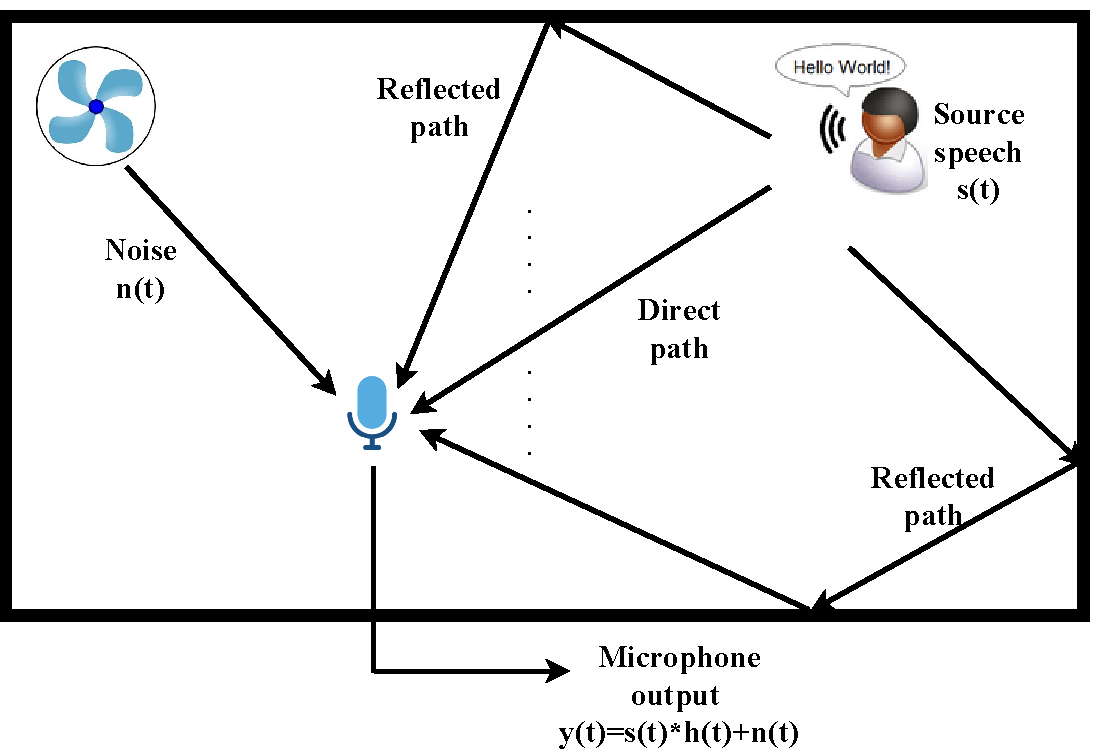
\includegraphics[width=\linewidth]{DSR_scenario.pdf}
\caption{DSR scenario}
\label{fig:DSR_scenario}
\end{figure}

\section{Reverberation}
Speech originating from a source placed distant from the receiving microphone undergoes multiple reflections. The microphone output will be the superposition of original source along with these delayed and attenuated versions of the original source. This effect is known as reverberation. The reverberated speech $y_R(n)$ can be represented as convolution of clean speech $s(n)$ and room impulse response (RIR) $h(n)$. Mathematically,
\begin{equation}
y_R(n)=h(n)*s(n) = \sum_{l=0}^{L-1}h(l)s(n-l),
\end{equation}
where $L$ represents the number of taps used to represent $h(n)$. Reverberated speech is assumed to be additive with noise. Mathematically, degraded speech $y(n)$ due to the effects of reverberation and noise can be represented as,
\begin{equation}
y(n)=y_R(n)+z(n)=h(n)*s(n)+z(n),
\end{equation}
where, $z(n)$ represents the noise. The effects of reverberation is different from the effects of echo.

The effects of reverberation depends on the properties of clean speech as well as RIR. Since reverberation dependent on the original source (clean speech), compensating for the effects of reverberation and blindly estimate the clean speech will be challenging.  

Speech originating from a source undergoes multiple reflections in a closed room. When this speech is captured using a microphone distant from the source (typically 30 cm to few meters), the microphone output is a superposition of the speech along with the delayed and attenuated copies of the signal referred to as reverberated speech~\cite{naylor2010speech}. Additionally, the microphone will capture background noise originating from other sources. The resulting microphone output in such a distant speech recording (DSR) setting is a degraded version of the original speech signal. The presence of such degradations impedes speech intelligibility~\cite{kinoshita2016summary}  and automatic speech recognition (ASR)~\cite{barker2018fifth, barker2015third} performance. The amount of degradation depends on the source and microphone positions, characteristics of the room and the noise~\cite{naylor2010speech,kinoshita2016summary}. To improve performance, it is desirable to compensate for these degradations.
\iffalse
\begin{itemize}
\item What is it ?
\item Representation using RIR
\item Differentiate reverberation from echo
\item Why it is challenging ?
\item Combined effect with noise
\end{itemize}
\fi
\section{Objective of the thesis}
\begin{itemize}
\item Improve speech quality of a single-channel DSR recording
\item Compensation for reverberation and noise
\item Improve ASR
\end{itemize}

\section{Contributions}
The main contribution of this work is incorporating various properties of the RIR spectrogram in a NMF based framework for dereverberation and denoising. Three different approaches to incorporate different properties of the RIR spectrogram are discussed in this work. Firstly, the cost function for NMF based dereverberation method is modified to introduce three different RIR structures - sparsity, frequency envelope and early part of the RIR spectrogram. The second part of the work proposes a NMF based speech enhancement method based on separability approximation on the RIR spectrogram. The model helps in separating the temporal and frequency effects of reverberation on clean speech and improving the speech enhancement results. The third work utilizes the low-rank nature of the RIR spectrogram to represent the joint effect of reverberation and noise using a NMF model. Further, an algorithm based on this model is shown to improve speech enhancement and ASR results when compared with other NMF based approaches in the literature.

\iffalse
\begin{itemize}
\item incorporate various constraints on RIR spectrogram in a NMF based dereverberation framework
\begin{itemize}
\item model sparsity, frequency envelope, early part of RIR
\item incorporate the constraints in cost function
\end{itemize}
\item A novel NMF based method to handle reverberation and noise jointly
\begin{itemize}
\item propose NMF models for RIR spectrogram (separability assumption, low-rank model)
\item incorporate these models along with NMF models for clean speech and noise spectrograms
\item better constrained model resulting in proper RIR and clean speech estimates
\item improvement in enhancement and ASR results
\item better understanding of effects of reverberation on clean speech bases and activations
\end{itemize}
\end{itemize}
\fi
\section{Organization of thesis}
Figure~\ref{fig:Thesis_chapters} shows the organization of rest of the thesis. Chapter~\ref{chapter:lit} reviews various speech dereverberation and denoising methods in literature. Chapter~\ref{chapter:rir} describe some of the time and frequency domain structure of RIR. These structure are utilized in this work. Chapter~\ref{chapter:icassp2017} discusses NMF based dereverberation methods that incorporates various meaningful constraints on RIR spectrogram. Chapter~\ref{chapter:interspeech2018} discusses a speech enhancement method based on separability assumption of the RIR spectrogram. Chapter~\ref{chapter:trans2020} discusses the speech enhancement method based on low-rank approximation of the RIR spectrogram. In Chapter~\ref{chapter:conclusion}, the work is concluded with discussions and possible future directions in incorporating these methods for other applications.
\begin{figure}
\centering
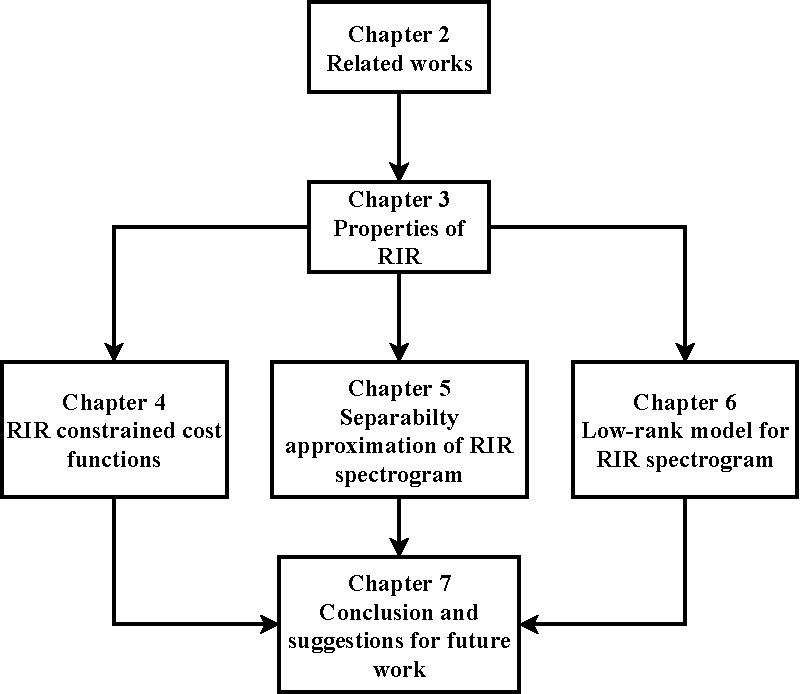
\includegraphics[width=\linewidth]{Thesis_chapters.pdf}
\caption{Thesis chapters}
\label{fig:Thesis_chapters}
\end{figure}


\chapter{Related Works}
\label{chapter:lit}
This chapter discusses various speech enhancement methods available in the literature. The different class of dereverberation methods available in the literature is summarized in Section~\ref{sec:dereverb_methods}. Since this work is based on NMF based model for reverberation and noise, the NMF based enhancement methods in the literature are explained in Section~\ref{sec:NMF_methods}.
%In this chapter we discusses various dereverberation methods available in literature. The different class of dereverberation methods available in literature is summarized in Section~\ref{sec:dereverb_methods}. Since this work is based on NMF based model for  reverberation and noise, the NMF based enhancement methods in literature are explained in Section~\ref{sec:NMF_methods}.

\section{Dereverberation methods}
\label{sec:dereverb_methods}


This section discusses various dereverberation methods in literature. Many of these methods can be extended to hande reverberation in presence of noise. The dereverberation methods can be broadly classified into - (i) beamforming, (ii) inverse filtering based methods, and (iii) reverberation suppression methods. Each methods are discussed in details next.

\subsection{Beamforming}

Beamforming is a multi-channel method. It utilizes the spatial information of the source and microphone array to enhance degraded speech recordings. A beamformer enhances the signal received from a particular direction and attenuates the signal received from other directions~\cite{naylor2010speech}. This spatial filtering is made possible by the fact that the sound waves travel an additional distance to reach distant microphones when compared with nearer microphones. This result in a relative time lag is referred to as time delay of arrival (TDAO). TDOA depends on the source position and microphone array configuration. 

Figure~\ref{fig:TDOA} illustrates the occurrence of TDOA for a source paced distant from a two-microphone array. 
The source is placed at an angle $\theta$ from the axis of the microphone array (referred to as incident angle). The signal travels an extra distance of $d\text{cos}(\theta)$ to reach microphone $M_1$ when compared with the reference microphone $M_{ref}$. This results in a time lag $\tau$ of
\begin{equation}
\tau = \dfrac{d \text{cos}(\theta)}{v}\text{,}
\end{equation}
where $v$ is velocity of sound in the medium. It can be observed that TDOA changed with the incident angle $\theta$ and microphone spacing $d$. 
\begin{figure}
\centering
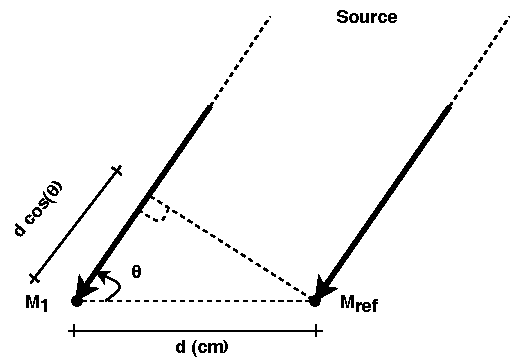
\includegraphics[width=\linewidth]{TDOA_plot.pdf}
\caption{ Two-microphone DSR recording setup. Microphones are placed $d$-distant apart. The effects of reverberation and noise is not shown in the figure.}
\label{fig:TDOA}
\end{figure}

Delay-sum beamforming (DSB) is the most straight forward beamforming approach. The microphone recordings are delayed to compensate for different TDOAs and a convex combination of these signals is taken. For a $M$-microphone array, the enhanced signal $\hat{x}(n)$ obtained using DSB can be summarized as,
\begin{equation}
\hat{x}(n)=\sum_{m=1}^M p_m x_m(n-\tau_m) \text{,}
\end{equation}
where $x_m(n)$ is the recording for $m$-th microphone. $p_m$ and $\tau_m$ represents the weight and TDOAs obtained for each microphone. $p_m$ can be fixed based on some amplitude normalization criteria~\cite{anguera2007acoustic}. $\tau_m$ can be estimated based on the source localization algorithms like generalized cross-correlation with phase transform (GCC-PHAT)~\cite{knapp1976generalized}. The signals from look-direction in different channels will add constructively. This results in enhancing signals coming from look-direction at the expense of the signals received from other directions.  Beamforming was shown to effectively suppress localized noise. However, reverberant speech is partially suppressed. Reverberation makes localized speech sources into diffused sound. The resulting reverberated speech signal reaches the array from all directions. Hence, reverberated speech signal coming from look direction will not be suppressed, while from other directions will be suppressed. 
 
Many modifications were proposed to improve the performance of the beamformer. MVDR beamforming uses noise statistics to improve performance. The effects of reverberation were suppressed with the use of multiple beamformers. This is achieved with the use of a three-dimensional microphone array. One beam is steered in the direction of the desired location as was the case in earlier.  Additional beams are steered in the direction of the strong initial reflections~\cite{nishiura2001speech} which acts as virtual sources. Another method to suppress reverberation was the use of a matched filter beamformer where the microphone responses are convolved with time-reversed RIR. The method requires Reverberation suppression methods model the effect of reverberation on the clean speech in some domains like the short-time Fourier transform (STFT), the residual signal obtained from linear prediction analysis, etc. Based on these models, algorithms are proposed to reduce the effects of reverberation. This results in a better estimate of clean speech. The approaches include spectral subtraction~\cite{lebart2001new}, weighted linear prediction (WPE)~\cite{nakatani2010speech}, Triple-N ICA for convolutive mixtures (TRINICON)~\cite{buchner2007trinicon}, linear prediction based method~\cite{naylor2010speech}, and NMF based approaches~\cite{kameoka2009robust}, information about RIR~\cite{naylor2010speech}.

\subsection{Inverse filtering based methods}
Inverse filtering based methods are multi-channel speech enhancement methods~\cite{naylor2010speech}. These methods have two steps - (i) blind estimation of RIR and (ii) inverse filtering.
\subsubsection{(i) Blind estimation of RIR}
\label{sec:MINT}
In this step, a blind estimate for RIR from the source to at least one of the microphones in the array is obtained. The correlation between speech recorded by different microphone channels is used for the purpose. Consider two channels DSR recording case degraded by reverberation alone. The microphone outputs $y_{R,1}$ and $y_{R,2}$ represented as,
\begin{align}
y_{R,1}(n)&=s(n)*h_1(n) \text{  and } \nonumber \\
y_{R,2}(n)&=s(n)*h_2(n)
\end{align}
where $s(n)$ is the clean speech, and $h_1(n)$ and $h_2(n)$ represents the RIRs form the source to the first and the second microphone, respectively. The microphone outputs are correlated based on the following relation.
\begin{align}
y_{R,1}(n)*h_2(n)&=(s(n)*h_1(n))*h_2(n) \nonumber \\
                 &=h_1(n)*(s(n)*h_2(n)) \nonumber \\
                 &=y_{R,2}(n)*h_1(n) \nonumber\\
y_{R,1}(n)*h_2(n)&-y_{R,2}(n)*h_1(n)=0
\label{eq:rir_cancel}
\end{align}
Based on (\ref{eq:rir_cancel}), a system of equations of the following form can be written~ \cite{xu1995least}.
\begin{equation}
\mathbf{Rh}=\mathbf{0}
\label{eq:system_eq}
\end{equation}
where, $\mathbf{R}$ represents a correlation-like matrix obtained from source signal $s(n)$~\cite{huang2003class}. $\mathbf{0}$ represents a zero vector. The vector $\mathbf{h}$ is obtained from RIRs as $\mathbf{h}=[\mathbf{h}_1^T|\mathbf{h}_2^T]^T$, where $h_1(n)$ and $h_2(n)$ form the elements of $\mathbf{h}_1$ and $\mathbf{h}_2$, respectively. The ideal solution for the $\mathbf{h}$ in the system of equations (\ref{eq:system_eq}) is the eigen-vector corresponding to the zeroth eigen-value in $\mathbf{R}$. In the presence of noise, the solution for $\mathbf{h}$ is eigen-vector corresponding to the smallest eigen-value. The system of equations in (\ref{eq:system_eq}) can be generalized for more microphone recordings are available.

Different approaches have been proposed in the literature to blindly estimate RIR based on the system of equations in (\ref{eq:system_eq}). Such methods assume that certain identifiability conditions and practical considerations are met~\cite{naylor2010speech}. Some of these methods are explained here. In~\cite{huang2003class}, a least-squares (LS) approach was proposed to solve the system of equations in (\ref{eq:system_eq}). The method based on eigendecomposition was also been proposed~\cite{gurelli1995evam}. In~\cite{gannot2003subspace}, full bands and frequency sub-bands eigendecomposition methods were proposed to solve for (\ref{eq:system_eq}) in the presence of white and colored noises. Adaptive filter in time domain~\cite{huang2002adaptive}  and frequency domain~\cite{huang2003class} were also proposed in literature.

\subsubsection{(ii) Inverse filtering}
\label{sec:inverse_fitering}
Inverse filtering methods could be used to estimate clean speech $s(n)$ from reverberated microphone recordings $y_{R,m}(n)$ and an estimate of RIRs $h_m(n)$. The most straight forward method would be to use an inverse filter $\mathbf{G}_m$ that  compensate for effects of reverberation as shown next.
\begin{equation}
\mathbf{y}_m^T\mathbf{G}_m=\alpha_0 \delta(n-n_0)\text{,}
\label{eq:direct_inversion}
\end{equation}
where $\alpha_0$ and $n_0$ represent arbitrary scaling and delay factors, respectively. $\delta(n)$ represents unit discrete delta function. However, the use of the direct inverse system shown in (\ref{eq:direct_inversion}) is challenging because of the following factors.  (i) RIR has non-minimum phase characteristics~\cite{neely1979invertibility}, (ii) spectral nulls can be present RIR spectrum and (iii) estimated inverse filter will have thousands of coefficients that require high precision and computationally expensive methods. In~\cite{mourjopoulos1982comparative}, inverse filter estimate $\hat{\mathbf{G}}_m$ was obtained based on a LS method. The estimated inverse filter minimizes the following cost function.
\begin{equation}
\hat{\mathbf{G}}_m = \underset{\mathbf{G}_m}{\text{min}} \left\lVert \mathbf{h}_m^T\mathbf{G}_m - \delta(n-n_0) \right\rVert_2^2
\end{equation} 
Homomorphic inverse filtering methods were also been investigated~\cite{radlovic2000nonminimum,mourjopoulos1982comparative}. The inverse filter was decomposed into minimum-phase and all-pass components. The minimum-phase component can be directly estimated from the magnitude spectrum of estimated RIR. Various methods like matched filtering~\cite{radlovic2000nonminimum} were used to estimate the all-pass components. 

When multi-channel RIRs are available, multiple-input/output inverse theorem (MINT) based approaches can be used to find exact inverse filters~\cite{miyoshi1988inverse}. According to the theorem, if the transfer function of two RIRs does not have any common zeros, then there exist a pair of inverse filters $\mathbf{G}_1$ and $\mathbf{G}_2$  such that
\begin{equation}
\mathbf{h}_1^T\mathbf{G}_1+\mathbf{h}_2^T\mathbf{G}_2=\delta(n)
\label{eq:MINT}
\end{equation}
In~\cite{miyoshi1988inverse}, a LS method was used to solve for (\ref{eq:MINT}). An exact inverse filtering can be performed by using an inverse filter length similar to that of RIR length. A sub-band version was proposed in~\cite{yamada1991recovering}. An adaptive version of the method is proposed in~\cite{nelson1995inverse}. Regularization was imposed on equalization problem in (\ref{eq:MINT}) to improve the robustness against noise and estimation errors~\cite{naylor2010speech}. 

\subsection{Reverberation suppression methods}
Reverberation suppression methods are based on modeling the effect of reverberation on clean speech in some domains. The commonly used domains are the short-time Fourier transform (STFT) and its variants, the residual signal obtained from linear prediction analysis, etc. Based on these degradation models, algorithms were proposed to reduce the effects of reverberation. This results in a better estimate of clean speech. The approaches include spectral subtraction~\cite{lebart2001new}, weighted linear prediction (WPE)~\cite{nakatani2010speech}, Triple-N ICA for convolutive mixtures (TRINICON)~\cite{buchner2007trinicon}, linear prediction based method~\cite{naylor2010speech}, and NMF based approaches~\cite{kameoka2009robust}, etc. SuchTypically these algorithms are single-channel methods. However, these methods can easily be extended for a multi-channel scenario.

\section{NMF based dereverberation methods}
\label{sec:NMF_methods}

NMF based speech enhancement methods are based on the modulation transfer function (MTF) model for reverberation. The MTF model states that for each frequency sub-band, the power envelope of the reverberated speech $\mathbb{Y}_R(k,n)$ is the convolution of power envelopes of clean speech $\mathbb{S}(k,n)$ and RIR $\mathbb{H}(k,n)$ for that particular sub-band. Mathematically,
\begin{equation}
\mathbb{Y}_R(k,n)=\mathbb{H}(k,n)*_n\mathbb{S}(k,n)=\sum_{l=0}^{L_h-1}\mathbb{H}(k,l)\mathbb{S}(k,n-l)\text{,}
\label{eq:MTF_model}
\end{equation}
where $*_n$ represents convolution along the time axis. $L_h$ represents the number of frames used to represent the RIR spectrogram. This model is valid when the reverberation condition does not change with time. Further, the MTF model is obtained by ignoring the cross-band effects occurring due to windowing~\cite{avargel2007system}.  The RIR phase spectrogram is also assumed to be uniformly distributed in the range $[-\pi, \pi)$.
Even though these approximations in the MTF model can pose a limitation for the dereverberation task, many dereverberation methods use this model. An additional advantage of the MTF model is that it avoids the need for a phase estimate for the RIR. Obtaining the phase spectrogram is difficult, especially if the recording is noisy~\cite{kameoka2009robust}. Estimation of $\mathbb{H}(k,n)$ and $\mathbb{S}(k,n)$ from $\mathbb{Y}_R(k,n)$ in (\ref{eq:MTF_model}) is viewed as solving for a CNMF problem. The dereverberated speech obtained using this algorithm showed improvements in speech enhancement instrumental measures.

Many modifications were proposed to improve the performance. The use of a magnitude spectrogram instead of a power spectrogram showed superior performance~\cite{Kumar2011}. The magnitude spectrogram of reverberated speech $\mathbf{Y}_R$ is expressed as a convolution of magnitude spectrograms of clean speech $\mathbf{S}$ and RIR $\mathbf{H}$. Mathematically,
\begin{align}
\mathbf{Y}_R&=\mathbf{H}*_n\mathbf{S} \nonumber \\
Y_R(k,n)& = \sum_{l=0}^{L_h-1} H(k,l)S(k,n-l) \text{,}
\label{eq:cnmf0}
\end{align}
where, $Y_R(k,n)$ $H(k,n)$, and $S(k,n)$ represents the elements of $\mathbf{Y}_R$, $\mathbf{H}$ and $\mathbf{S}$, respectively. Further, it was shown that the use of gamma-tone filter banks helped in improving ASR results when compared with the use of uniform filter banks. 

The reverberation model in (\ref{eq:cnmf0}) did not use any model for the clean speech spectrogram. Introducing clean speech spectrogram models were shown to improve speech enhancement results.  In~\cite{mohammadiha2016speech, Mohammadiha2015}, a NMF model for the clean speech spectrogram $\mathbf{S}$ was incorporated in the reverberation model in (\ref{eq:cnmf0}). The NMF model of clean speech spectrogram can be written as,
\begin{align}
\mathbf{S}&= \mathbf{W}_s\mathbf{X}_s \nonumber \\
S(k,n)    &= \sum_{r=1}^{R_s} W_s(k,r)X_s(r,n)\text{,}
\label{eq:NMF_clean_speech}
\end{align}
where, $\mathbf{W}_s$ and $\mathbf{X}_s$ represents bases and activation matrices obtained by performing NMF decomposition on the clean speech spectrogram $
\mathbf{S}$, respectively. $R_s$ represents the rank of NMF decomposition. $W_s(k,r)$ and $X_s(r,n)$ represents the elements of $\mathbf{W}_s$ and $\mathbf{X}_s$, respectively. Incorporating the clean speech model (\ref{eq:NMF_clean_speech}) in the reverberation model in (\ref{eq:cnmf0}) results in a reverberation model that can be written as,
\begin{equation}
Y_R(k,n) = \sum_{l=0}^{L_h-1} H(k,l) \bigg[ \sum_{r=1}^{R_s} W_s(k,r) X_s(r,n-l) \bigg]
\label{eq:cnmf1}
\end{equation}
Iterative algorithm were proposed to estimate clean speech spectrogram. There were two approaches depending on how clean speech bases $\mathbf{W}_s$ is learned - online approach and offline approach. In offline approach , the $\mathbf{W}_s$ is learned from reverberated spectrogram. In online approach, $\mathbf{W}_s$ is pre-learned from a set of clean speech utterances. A NMF decomposition is performed on the magnitude spectrogram of these clean speech utterances to estimate $\mathbf{W}_s$. Many constraints on the estimated clean speech like sparsity~\cite{mohammadiha2016speech, Mohammadiha2015}, and continuity~\cite{wager2018collaborative} were used to improve the performance. 

Representing clean speech spectrogram using CNMF model were also proposed to improve speech dereverberation perfromance~\cite{Mirsamadi2014}. In~\cite{Kallasjoki2014}, a NMF model for speech reverberation was proposed. This model is equivalent to the CNMF model for reverberation in (\ref{eq:cnmf1}). The bases matrix of the NMF decomposition is a structured matrix that was constructed to mimics the CNMF model.

The reverberation model in (\ref{eq:cnmf1}) is inappropriate to model reverberation in the presence of noise.  The model was modified by incorporating a noise model. The magnitude spectrogram of reverberated speech in the presence of noise $\mathbf{Y}$ was approximated as the sum of magnitude spectrograms of reverberated speech $\mathbf{Y}_R$ and noise $\mathbf{Z}$~\cite{li2018multichannel}. Mathematically,
\begin{align}
\mathbf{Y} &\approx \mathbf{Y}_R+\mathbf{Z} = \mathbf{H}*_n\mathbf{S}+\mathbf{Z}\nonumber \\
Y(k,n) &= H(k,n)*_n S(k,n) + Z(k,n) \text{,}
\label{eq:degradation_model}
\end{align}
where $Y(k,n)$ and $Z(k,n)$ represents the elements of $\mathbf{Y}$ and $\mathbf{Z}$, respectively. Similar to the NMF model for clean speech spectrogram in (\ref{eq:NMF_clean_speech}), a NMF approximation for noise spectrogram can be used as shown in (\ref{eq:NMF_noise}).
\begin{align}
\mathbf{Z}&= \mathbf{W}_n\mathbf{X}_n \nonumber \\
Z(k,n)    &= \sum_{r=1}^{R_n} W_n(k,r)X_n(r,n)\text{,}
\label{eq:NMF_noise}
\end{align}
where $\mathbf{W}_n$ and $\mathbf{X}_n$ were the bases and activation matrix of noise spectrogram $\mathbf{Z}$. $R_n$ represents the rank of NMF decomposition. $W_n(k,r)$ and $X_n(r,n)$ represents the elements of $\mathbf{W}_n$ and $\mathbf{X}_n$, respectively. The  degradation model in (\ref{eq:degradation_model}) is modified with the use of NMF models for clean speech in (\ref{eq:NMF_clean_speech}) and noise (\ref{eq:NMF_noise}) as shown next.
\begin{align}
\mathbf{Y} & = \mathbf{H}*_n \bigg[ \mathbf{W}_s\mathbf{X}_s \bigg]+\mathbf{W}_n\mathbf{X}_n
\label{eq:NMF_degradation_model}
\end{align}
Based on the degradation model in (\ref{eq:NMF_degradation_model}), a speech enhancement algorithm was proposed in~\cite{baby2016supervised}. The algorithm was a supervised approach where the clean speech and noise bases are assumed to be known. Exemplar-bases are learned for the purpose. This approach of obtaining the bases is different from the one used in~\cite{mohammadiha2016speech, Mohammadiha2015}. The use of the CNMF model for the clean speech and the noise spectrogram was also proposed in~\cite{baby2016supervised, baby2016phd}. The use of the CNMF model for the clean speech and the noise spectrogram was also proposed in~\cite{baby2016supervised, baby2016phd}. In~\cite{baby2016supervised}, the temporal variation of the RIR spectrogram was modeled along with the degradation model in (\ref{eq:NMF_degradation_model}).

\iffalse
\begin{itemize}
\item Reverberation methods: cost function, iterative procedure
\item Extending to noisy scenario - use of additive noise, extended model, results
\end{itemize}
\fi

\section{Limitations of NMF based dereverberation methods in literature}
The NMF based speech enhancement methods in literature utilize limited information about the RIR spectrogram.  This limits the performance of these algorithms. In this work different spectro-temporal models for the RIR spectrograms are proposed. Incorporating these novel RIR constraints on the NMF based enhancement algorithm helped in improving the performance. The reverberation models used in this work models the effects of reverberation on the magnitude spectrogram of clean speech. Hence, in the subsequent chapters, the usage of spectrogram means the magnitude spectrogram, unless stated otherwise. 
Chapter~\ref{chapter:rir} discusses the various properties of the RIR. Some of these properties are used in this work. The subsequent chapters discuss the different proposed speech enhancement algorithms that utilize these RIR models.  

\iffalse
\begin{itemize}
\item Most methods does not model RIR
\item Some methods use week constraints on RIR 
\item Thesis work is on incorporation various models for RIR in NMF based reverberation model
\item This resulted in improved enhancement and ASR results, proper RIR estimates 
\end{itemize}
\fi

\iffalse
Speech originating from a source undergoes multiple reflections in a closed room. When this speech is captured using a microphone distant from the source (typically 30 cm to few meters), the microphone output is a superposition of the speech along with the delayed and attenuated copies of the signal referred to as reverberated speech~\cite{naylor2010speech}. Additionally, the microphone will capture background noise originating from other sources. The resulting microphone output in such a distant speech recording (DSR) setting is a degraded version of the original speech signal. The presence of such degradations impedes speech intelligibility~\cite{kinoshita2016summary}  and automatic speech recognition (ASR)~\cite{barker2018fifth, barker2015third} performance. The amount of degradation depends on the source and microphone positions, characteristics of the room and the noise~\cite{naylor2010speech,kinoshita2016summary}. To improve performance, it is desirable to compensate for these degradations. The focus of this work is on jointly handling dereverberation and denoising. In this work we refer to methods that perform dereverberation in presence of noise as speech enhancement methods.

Dereverberation methods in literature can be broadly classified as (i) beamforming methods, (ii) inverse filtering methods and (iii) reverberation suppression methods. Many of these approaches can be extended to jointly handle reverberation and noise. (i) Beamforming is a multi-channel method. It uses a spatial filter that enhances speech incident from the desired direction and suppresses speech coming from other directions~\cite{gannot2017consolidated}. The multi-channel recordings are filtered and weighed to focus the beam to the desired direction. (ii) Inverse filtering methods blindly estimate the room impulse response (RIR) from the microphone recordings. Blind system identification approaches like the least-squares (LS) method and eigendecomposition method are used to blindly estimate the RIR~\cite{naylor2010speech}. This RIR is used to retrieve the original speech source. (iii) Reverberation suppression methods model the effect of reverberation on the clean speech in some domains like the short-time Fourier transform (STFT), the residual signal obtained from linear prediction analysis, etc. Based on these models, algorithms are proposed to reduce the effects of reverberation. This results in a better estimate of clean speech. The approaches include spectral subtraction~\cite{lebart2001new}, weighted linear prediction (WPE)~\cite{nakatani2010speech}, Triple-N ICA for convolutive mixtures (TRINICON)~\cite{buchner2007trinicon}, linear prediction based method~\cite{naylor2010speech}, and NMF based approaches~\cite{kameoka2009robust}, etc. In this work, a novel single-channel NMF based method to perform dereverberation and denoising jointly is proposed. Various NMF based enhancement methods proposed in literature are discussed next. 

NMF based dereverberation methods are based on the non-negative convolutive transfer function (N-CTF) model for the magnitude STFT of the reverberated speech ~\cite{kameoka2009robust,mohammadiha2016speech, Mohammadiha2015, Kumar2011}. For each frequency band, the temporal variation of reverberated speech is modeled as the convolution of magnitude spectrogram values of the clean speech and the RIR for that particular frequency. This model is valid when the reverberation condition does not change with time. Further, the N-CTF model is obtained by ignoring the cross-band effects occurring due to windowing~\cite{avargel2007system}.  Even though these approximations in the N-CTF model can pose a limitation for the dereverberation task, many dereverberation methods use this model. An additional advantage of the N-CTF model is that it avoids the need for a phase estimate for the RIR. Obtaining the phase spectrogram is difficult, especially if the recording is noisy~\cite{kameoka2009robust}. 

Based on the N-CTF model, a speech dereverberation algorithm was proposed in~\cite{kameoka2009robust}. Estimation of clean speech spectrogram is viewed as solving a CNMF problem. This algorithm shows improvements in speech enhancement instrumental measures. In~\cite{Kumar2011}, the N-CTF model for reverberation is extended for a gammatone filterbank. The estimated clean speech features are shown to improve ASR performance. In~\cite{Kallasjoki2014}, a NMF model for speech reverberation is proposed which is equivalent to the CNMF model for reverberation. The bases matrix of the NMF decomposition is a structured matrix that mimics the CNMF model. 
The dereverberation performance using the CNMF model was improved by introducing models for clean speech spectrograms like NMF~\cite{mohammadiha2016speech, Mohammadiha2015} and CNMF~\cite{Mirsamadi2014} models. Many constraints on the estimated clean speech are used like sparsity~\cite{mohammadiha2016speech, Mohammadiha2015}, and continuity~\cite{wager2018collaborative} to improve the performance.

The N-CTF model cannot be used as such for reverberated speech in the presence of noise. Including a noise model to the N-CTF model helps in improving the dereverberation performance. The magnitude spectrogram of reverberated speech in the presence of noise is approximated as the sum of magnitude spectrograms of reverberated speech and noise~\cite{li2018multichannel}. Using this model, with NMF models for clean speech and noise spectrograms, a supervised joint dereverberation and denoising algorithm was proposed in~\cite{baby2016supervised}. The use of the CNMF model for the clean speech and the noise spectrogram was also proposed in~\cite{baby2016supervised, baby2016phd}. All the enhancement methods based on N-CTF discussed above use models for clean speech spectrogram but do not use any specific models for the RIR spectrogram.

Use of meaningful constraints on the RIR spectrogram along with speech model will help the dereverberation methods. Some methods use a simple model for the RIR spectrogram. The temporal variation of the RIR spectrogram was modeled in~\cite{baby2016supervised}. The RIR spectrogram energy across frames was modeled to decay with time. Based on this RIR model, an enhancement algorithm was proposed in~\cite{baby2017joint}, to improve the speech enhancement results. This method does not consider the spectral variation of the RIR spectrogram. With the knowledge of the RIR, we had proposed in~\cite{mohanan2017speech}, the use of the sparse nature and the presence of a frequency envelope for the RIR spectrogram to improve the speech enhancement results. Further, in~\cite{mohanan201a}, a spectral and temporal model for the RIR spectrogram was proposed based on a separability approximation on the RIR spectrogram. The approximation resulted in a rank-$1$ NMF model for the RIR spectrogram. Based on the RIR model, the reverberated speech spectrogram is modeled using NMF as opposed to CNMF model used in literature.

In this work, we propose a NMF based approach to handle dereverberation and denoising jointly. Such an approach is different from other NMF based approaches that use a combination of CNMF and NMF for the purpose. The proposed model is easy to interpret. The spectral and temporal variation of the RIR is modeled using a low-rank NMF approximation of the RIR spectrogram. Even though such a representation reduces the number of parameters used for representing the RIR spectrogram, the enhancement results obtained are better than other NMF based approaches. Further, the approach is extended to work in unknown noise conditions. Such an approach gives better enhancement results when compared to existing NMF based dereverberation methods. As a byproduct, the RIR spectrogram estimates obtained using the proposed approach is better and closer to the true RIR spectrogram when compared to other NMF based approaches.

The main contribution of this paper is in incorporating a novel spectro-temporal model for the RIR spectrogram in the N-CTF model for reverberation. This model results in a NMF based algorithm to jointly handle dereverberation and denoising. Such a representation helps in imposing better constraints on the RIR spectrogram which was not possible in other NMF based methods. This resulted in superior enhancement results when compare with competing methods.
%The proposed algorithm showed superior enhancement results. 
This also resulted in a RIR estimate which is closer to the true RIR spectrogram.
\fi
\chapter{Properties of RIR}
\label{chapter:rir}
This chapter discusses various properties exhibited by RIR. The enhancement algorithms proposed in subsequent chapters incorporate these RIR properties. The time and frequency domain structure of RIR is discussed first. The later part discusses structures present in the RIR magnitude spectrogram. 

\section{Structure of RIR}
This section discusses time domain and frequency domain structure of RIR. 

\subsection{Time domain structure}
The Figure~\ref{fig:rir_time_domain} shows the time domain structure of a recorded RIR available from REVERB challenge database. The RIR has a $T_{60}\approx 700$~ms and source-microphone distance of $2$~m. A similar observations are obtained for other RIRs. The initial part of RIR consists of a short duration of near-zero amplitude that is followed by a peak. This peak represents the speech reaching the microphone due to direct-path propagation. Minimum energy loss occurs in direct-path propagation since it does not undergo absorption due to reflections from the walls. Hence this peak has a high amplitude. The near-zero amplitude region occurring before the peak amplitude corresponds to the direct-path propagation delay. The direct-path peak is followed by other peaks that correspond to the reflected paths. The peaks occurring near the direct-path peak occur due to the strong reflections from the walls. These peaks have relatively larger values when compared with later reflections. The overall structure of the RIR magnitude decays with time.  

The reverberant part of RIR is divided into two regions - early and the late reflections~\cite{naylor2010speech}. Such a distinction is made because of the unique effects caused by these regions on the clean speech. The reflections reaching the microphone with a delay of up to $50$~ms after the direct path from the early reflections. The reflections reaching after $50$~ms forms the late reverberation (reverberation tail). The early reflections are constituted by well-defined reflections and have larger amplitudes. 
The early refection mostly causes spectral changes to clean speech. This perceptual effect is referred to as spectral coloration. Early reflections are indistinguishable from direct-path sound due to the temporal masking of ears. This effect has shown to improve speech intelligibility. However, coloration degrades the quality of recorded speech~\cite{naylor2010speech,kuttruff2016room}. Reverberation tail has smaller amplitudes and diffused nature i.e., sound comes from all directions. The reverberation tail can extend for a longer duration and it gives a perception of sound 'ringing on' effect for a short duration before the reverberant speech starts decaying. This temporal smearing effect gives the impression of space and distance~\cite{naylor2010speech}. The reverberation tail is a major contributor to degradation in speech quality and deteriorates ASR performance.   
%The early refection mostly causes spectral changes to clean speech. This perceptual effect is referred to as spectral coloration. Early reflections are indistinguishable from direct-path sound due to the temporal masking of ears. This effect has shown to improve speech intelligibility. However, coloration degrades the quality of recorded speech~\cite{naylor2010speech,kuttruff2016room}. Reverberation tail has smaller amplitudes and diffused nature i.e., sound comes from all directions. The reverberation tail can extend for longer duration. It is a major contributor for degradation in speech quality and deteriorate ASR performance.  
\begin{figure}[ht!]
\centering
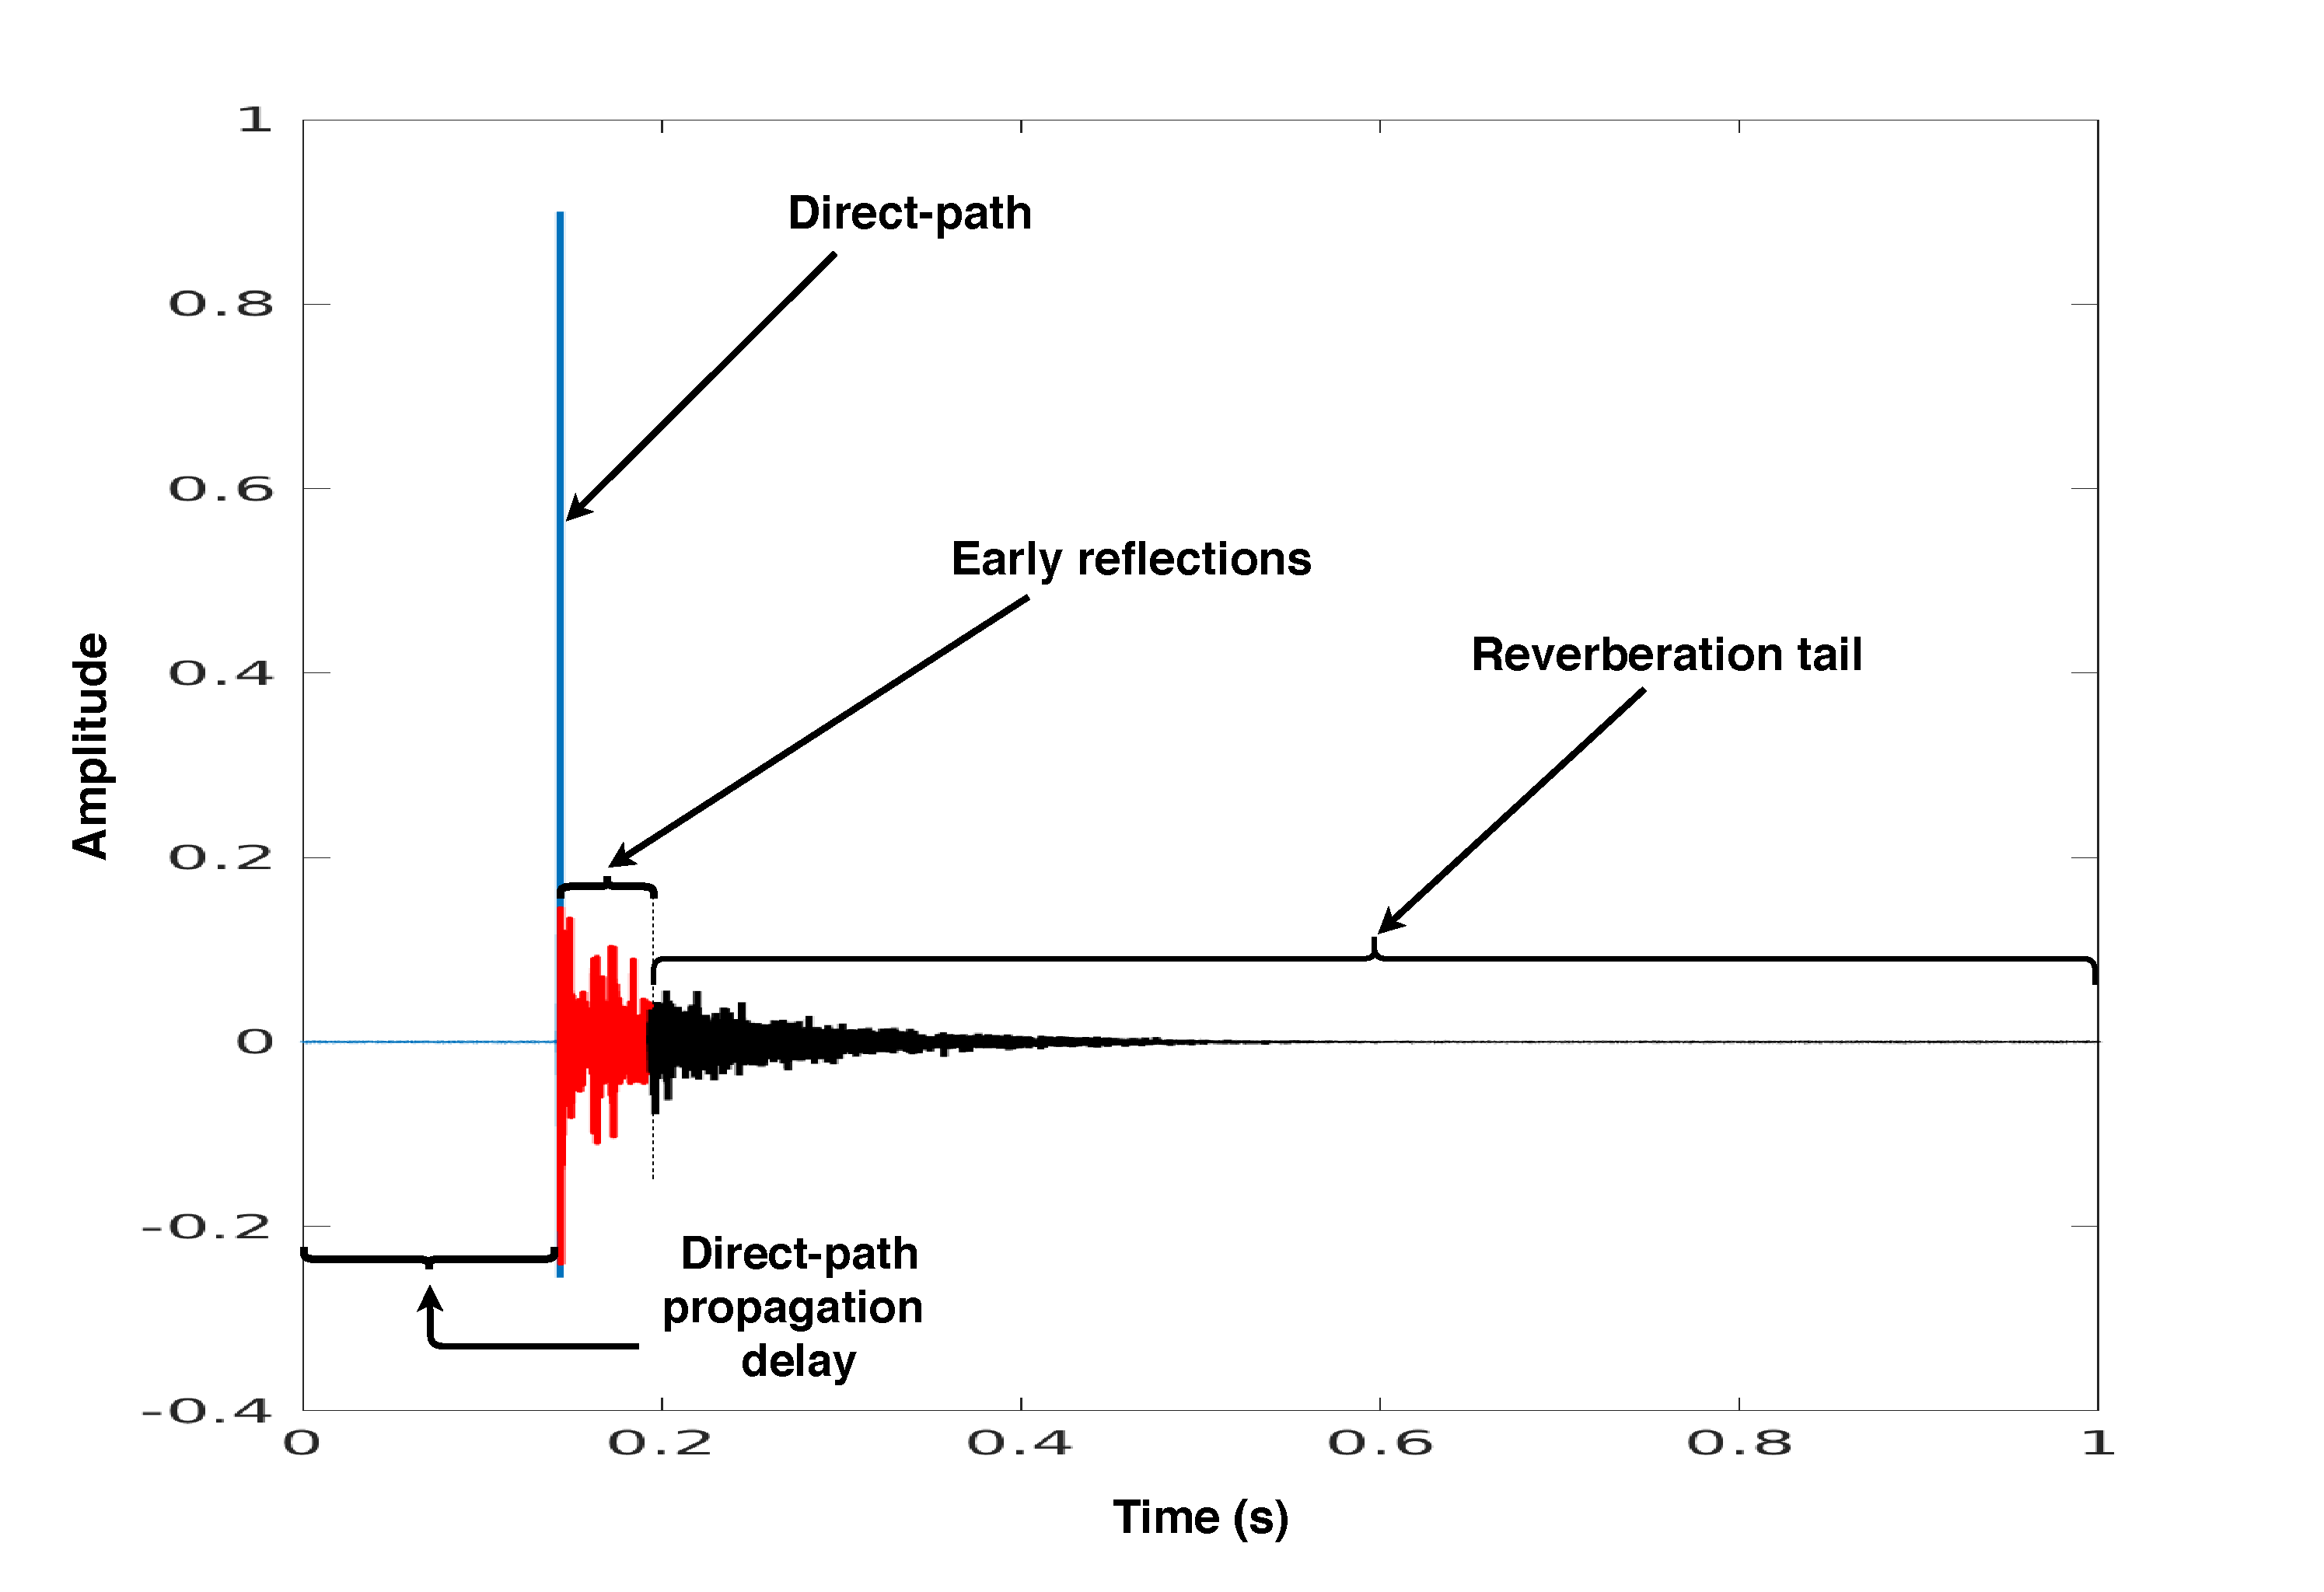
\includegraphics[width=\linewidth]{rir_time_domain.pdf}
\label{fig:rir_time_domain}
\end{figure}

\subsection{Magnitude spectrum of RIR}
The Figure~\ref{fig:rir_spectrum} shows the log-magnitude spectrum for the RIR shown in Figure~\ref{fig:rir_time_domain}. It can be observed that the average difference between spectral maximum and minimum is more than $10$~dB~\cite{kuttruff2016room}. The magnitude spectrum also exhibits spectra null for some frequencies. These effects imposes serious limitations on use of inverse filtering based approaches to compensate for the effects of reverberation.   
\begin{figure}[ht!]
\centering
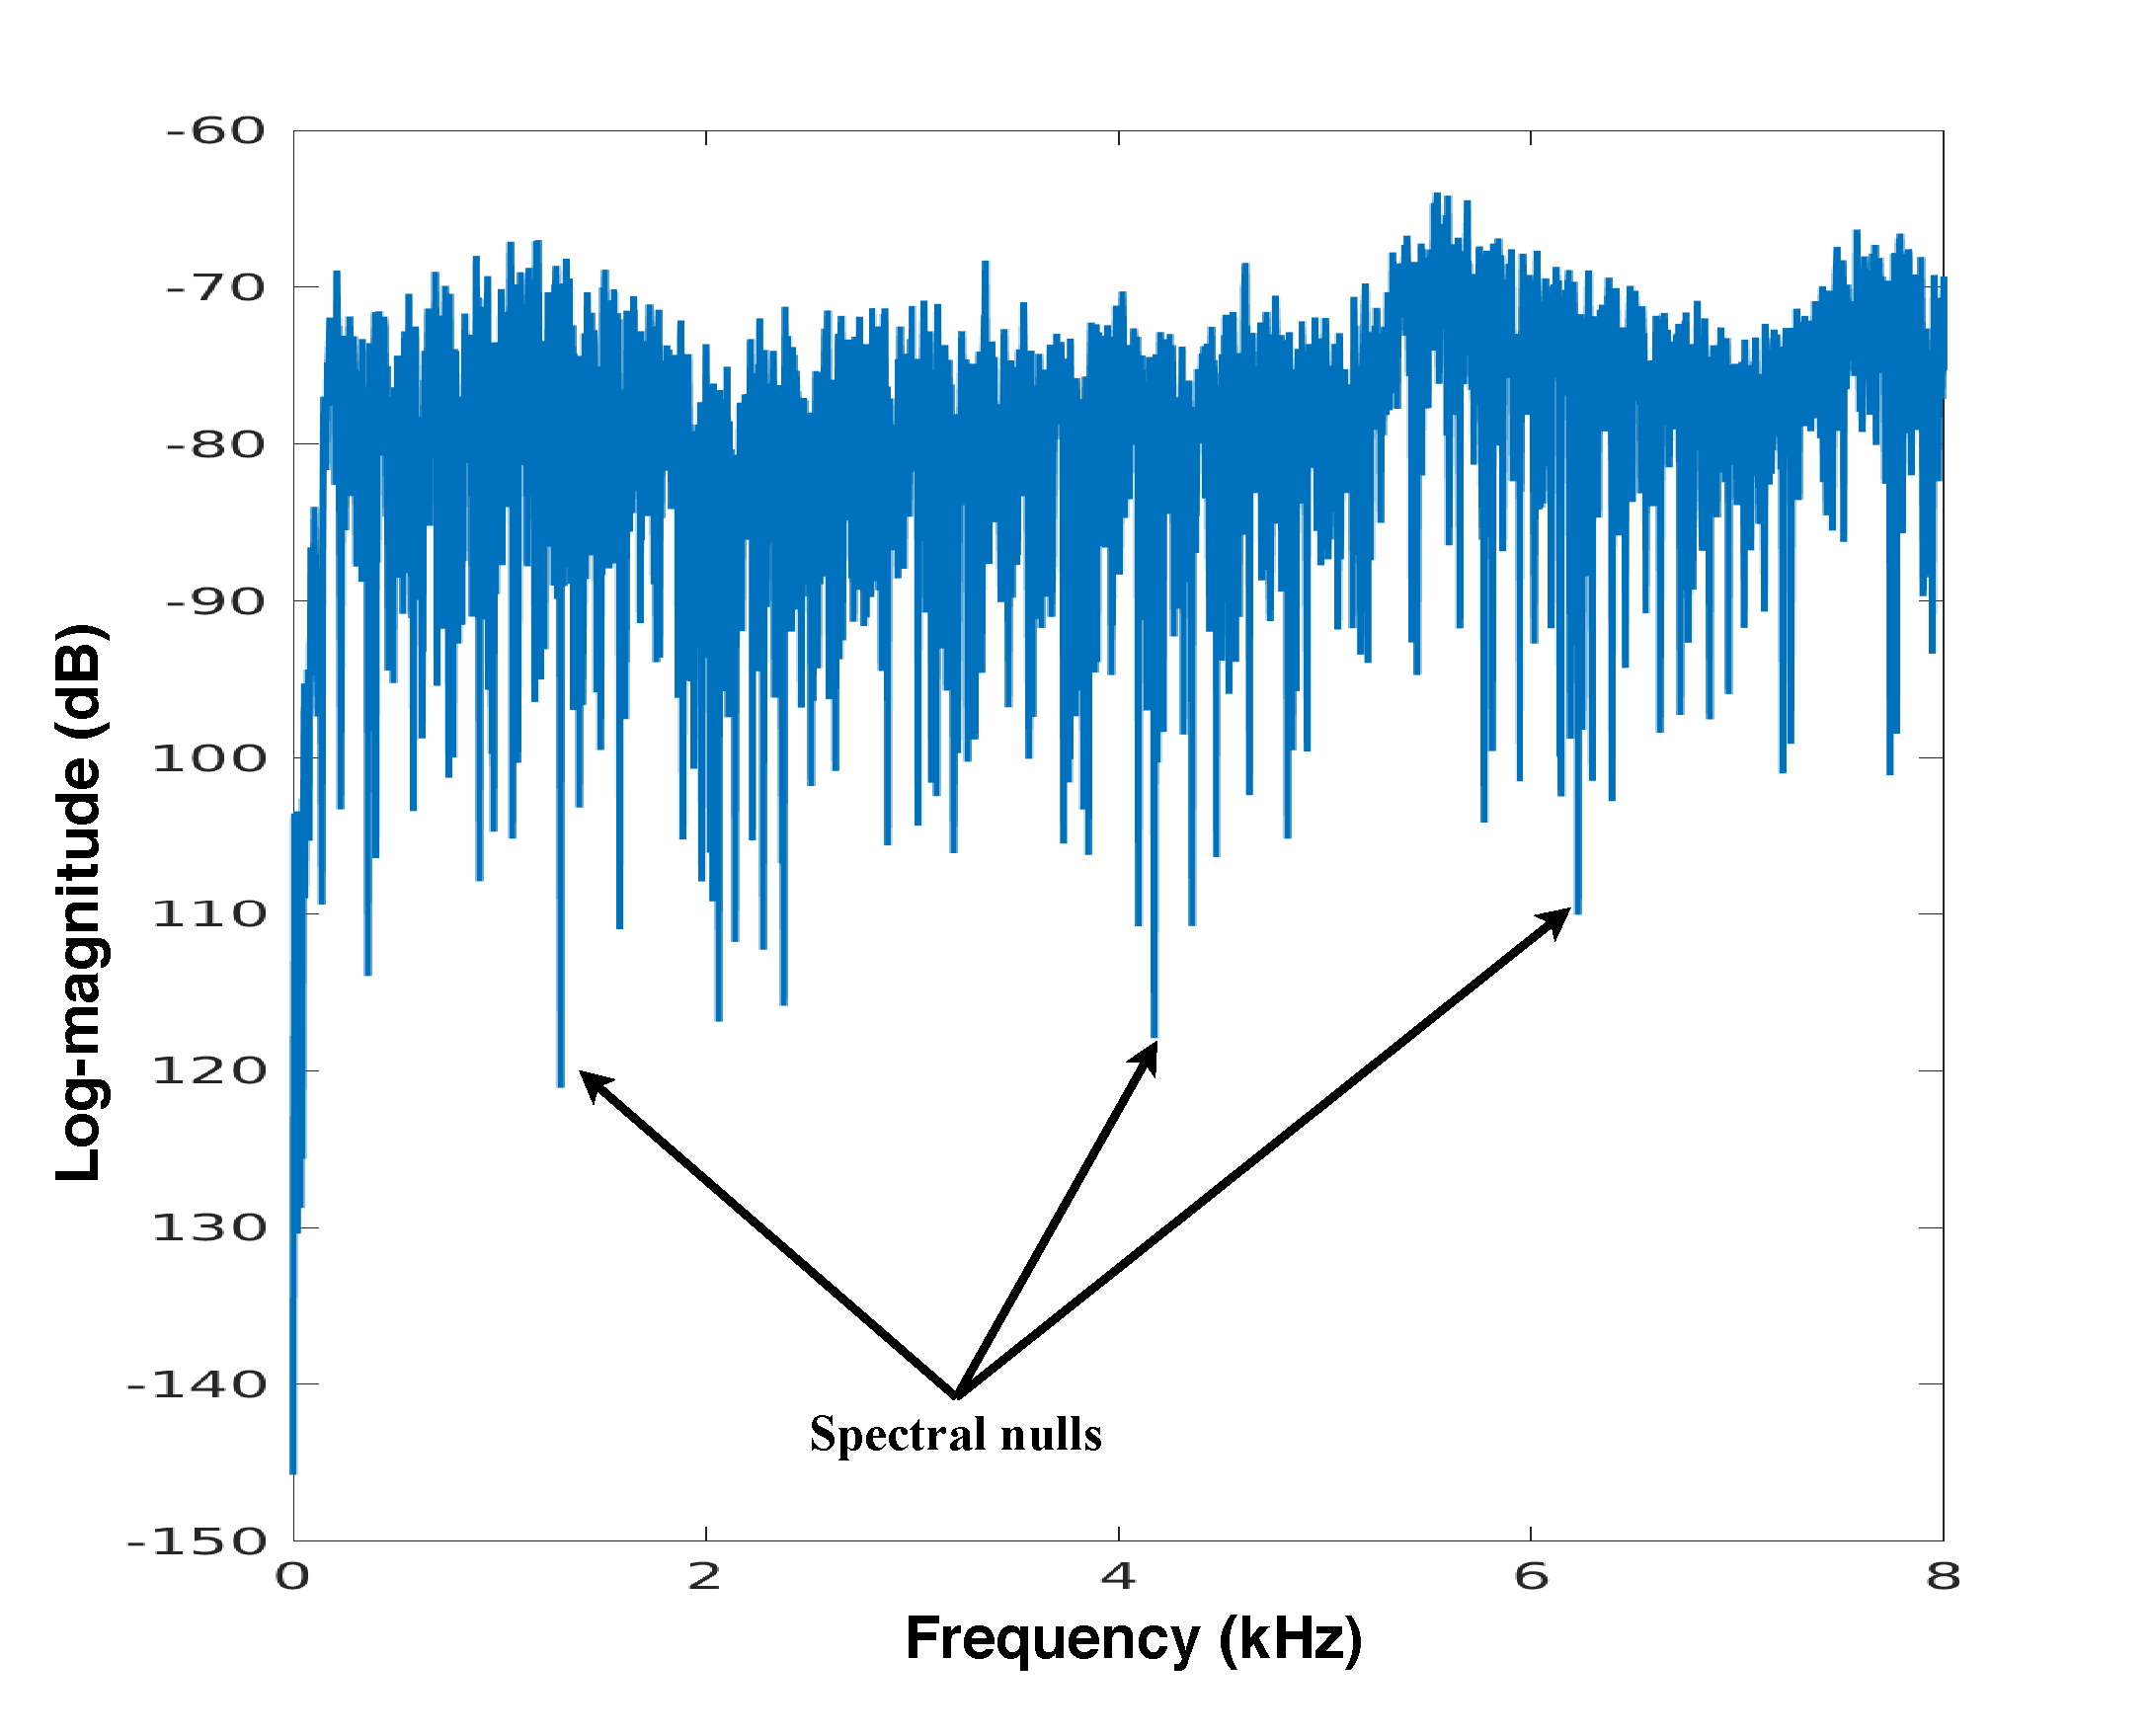
\includegraphics[width=\linewidth]{rir_spectrum.pdf}
\label{fig:rir_spectrum}
\end{figure}

\subsection{Pole-zero plot of RIR}
The Figure~\ref{fig:rir_pole_zero} shows the pole-zero plot for the RIR shown in figure~\ref{fig:rir_time_domain}~\footnote{The multiplicity of poles and zeros are not shown in the plot for simplicty as the non-minimum phase nature of RIR does not change with multiplicity.}. Most of the zeros are located near the unit circle. Out of these zeros, some lie inside the  unit circle while others lie out side the unit circle. This make the RIR a non-minimum phase system. Such an observation is observed for RIRs estimated for most real rooms~\cite{neely1979invertibility}.
\begin{figure}[ht!]
\centering
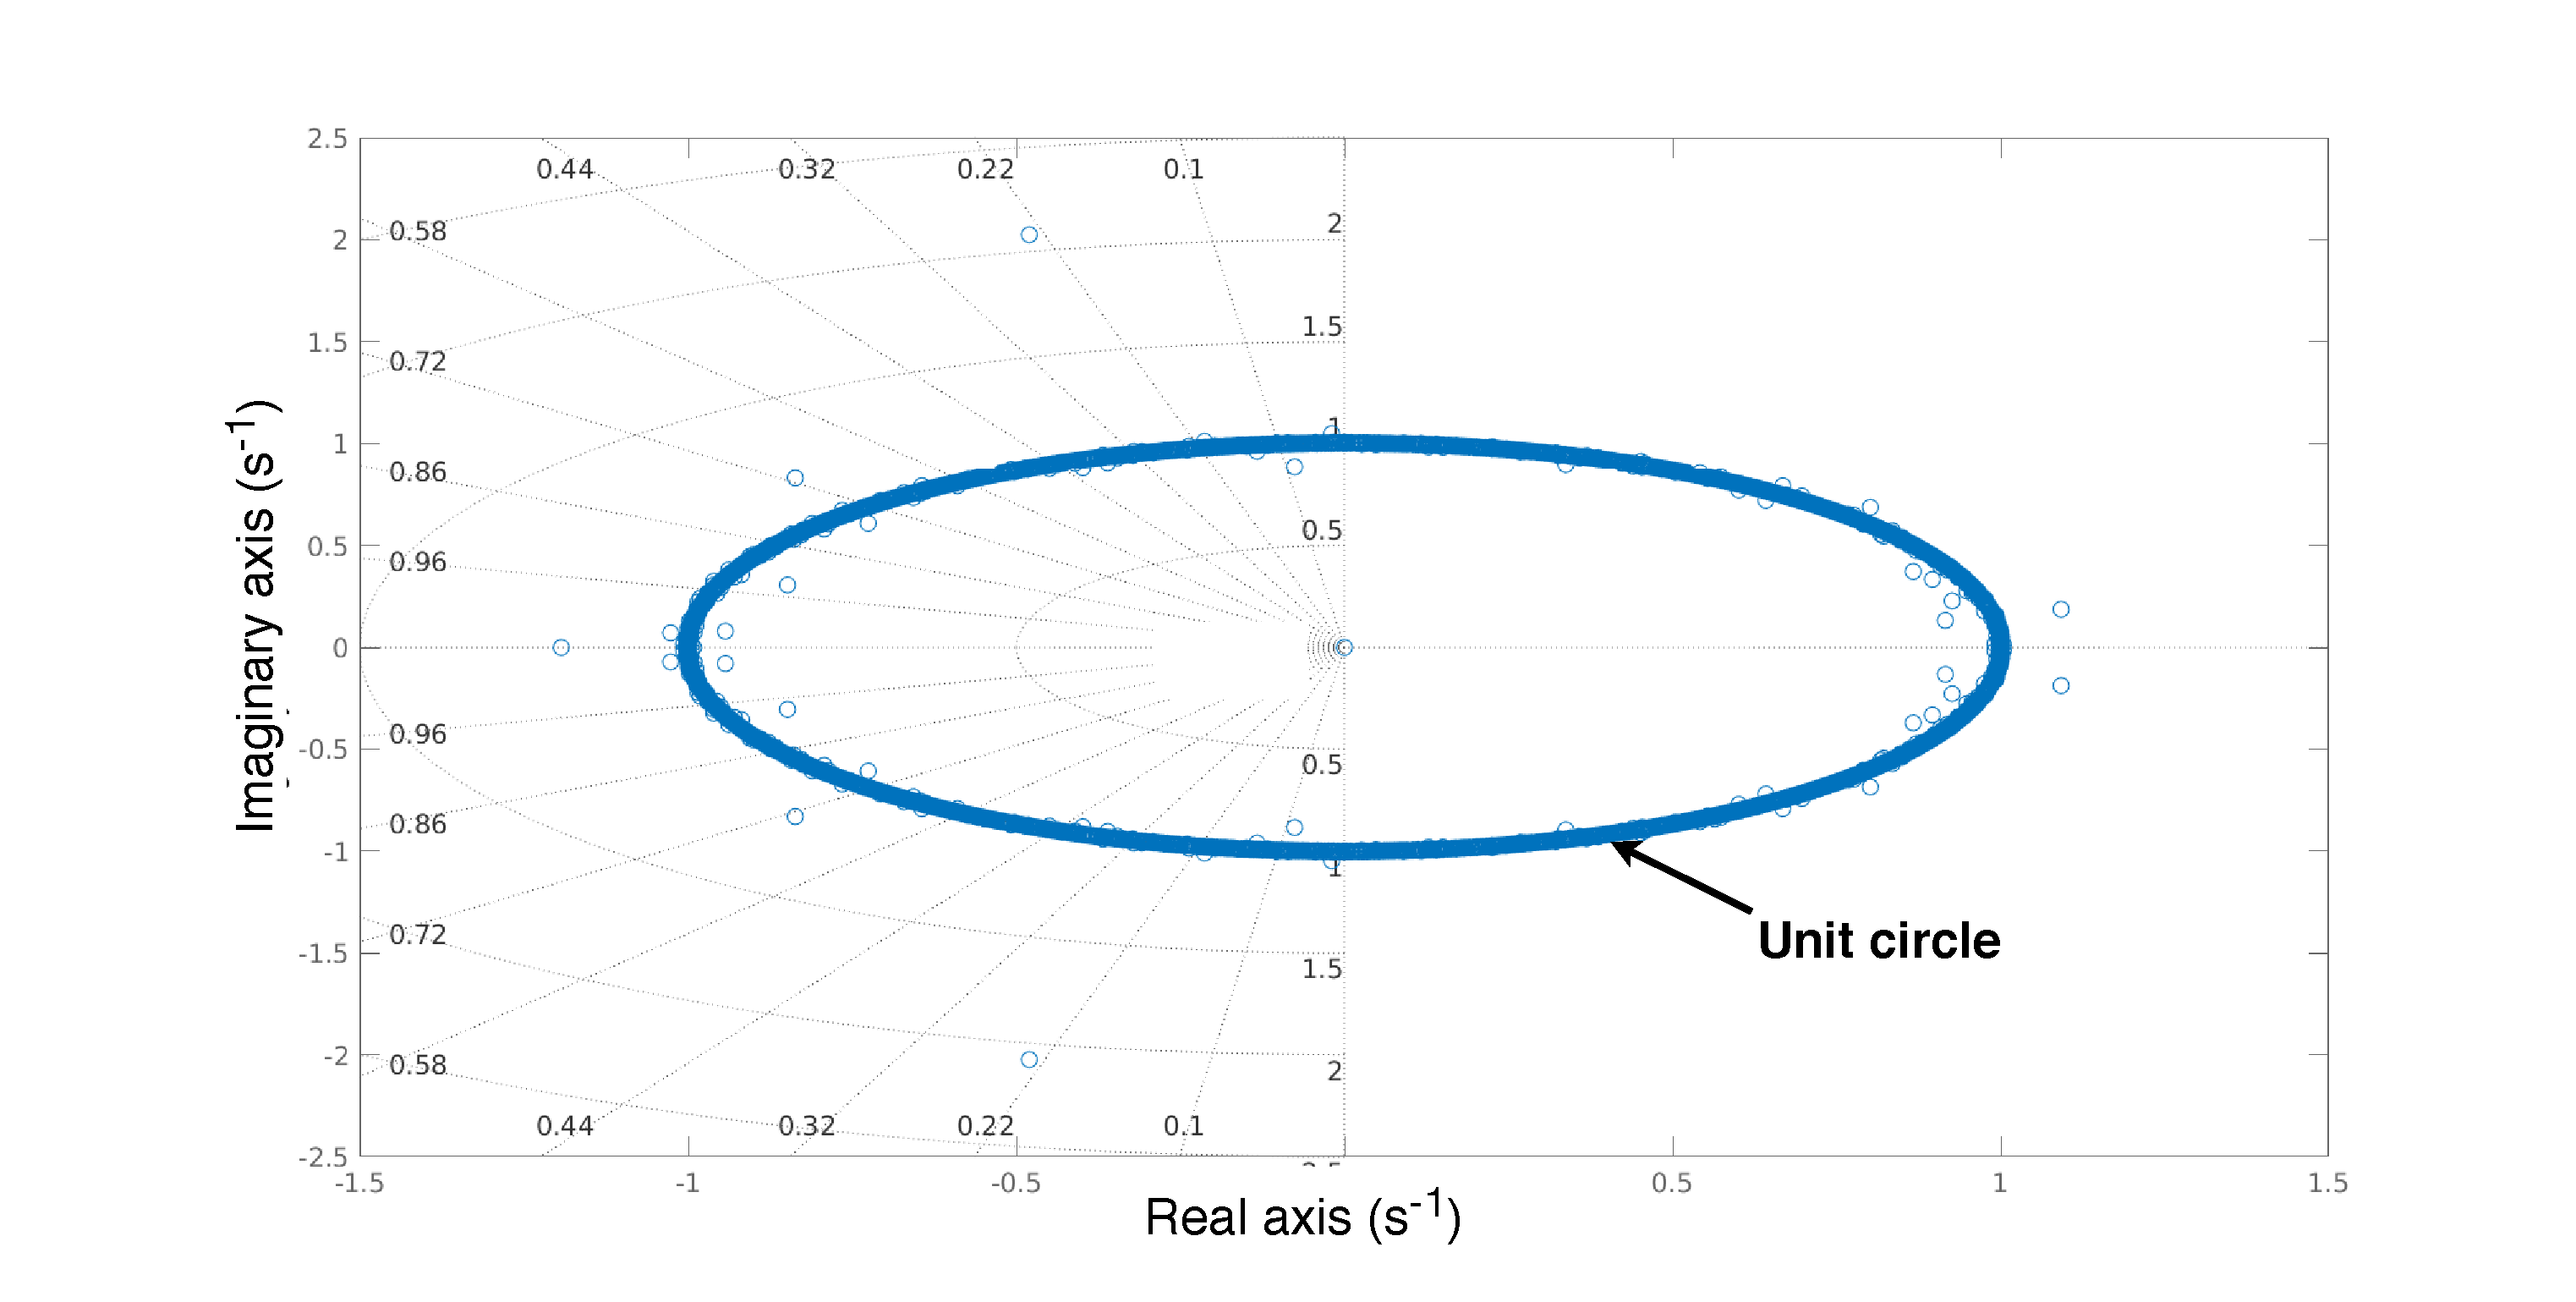
\includegraphics[width=\linewidth]{rir_pole_zero_plot.pdf}
\label{fig:rir_pole_zero}
\end{figure}

\subsection{Inverse filtering}
Inverse filtering is the most straight forward approach to compensate for the effects of reverberation. This approach depends on finding an inverse filter $g(n)$ such that it compensates the effects of RIR $h(n)$.
\begin{equation}
h(n)*g(n)=\alpha_i\delta(n-\tau_i)\text{,}
\label{eq:inv_filt}
\end{equation}
where $\alpha_i$ and $\tau_i$ represents arbitrary scaling and delay factor. This assumes that the RIR is known. The RIR can be estimated based on some methods discussed in Section~\ref{sec:inverse_fitering}. $g(n)$ can be obtained using the spectral analysis of (\ref{eq:inv_filt}). However, the direct application of inverse filtering is inappropriate because of the following reasons~\cite{naylor2010speech}. 
(i) the time-domain RIR is represented using thousands of coefficients. A similar number of coefficients are required to represent the inverse filter.  The estimation of such a high order system requires a robust algorithm with high numerical precision and computational cost. Further, even small errors in the RIR estimation (occurs especially in phase spectrum) can introduce a significant amount of artifacts in the estimated speech. In the presence of noise, the introduced artifacts will be more severe. 
(ii) The inverse filter is unstable as the RIR has a non-minimum phase response. 
(iii) The spectral nulls present in the RIR lead to strong peaks in the inverse filter. This leads to narrow-band noise amplification on the estimated dereverberated speech. 

The inverse filtering for multi-channel recordings is not as challenging as single-channel recording. For multi-channel recording of $M$ channels, utilizing MINT a set of stable inverse filters $g_m(n),m \in \{1,2,..,M\}$ can be obtained for the RIRs $h_m(n),m \in \{1,2,..,M\}$. Mathematically,
\begin{equation}
\sum_{m=1}^M h_m(n)*g_m(n) = \delta(n)\text{.}
\end{equation}
Various dereverberation methods based on MINT are discussed in Section~\ref{sec:MINT}.

As discussed previously, inverse filtering cannot be used for single-channel speech dereverberation. Singe-channel methods have to use various structures present in clean speech and RIR to perform speech dereverberation. Since the properties of clean speech and RIR (early part and reverberation tail) changes with time, short-time analysis is more fruitful. Short-time Fourier transform (STFT) and its variants are commonly used for this purpose. In this work various properties of magnitude STFT (magnitude spctrogram) of RIR is used. So, different properties of the RIR magnitude spectrogram is explained next.
\iffalse
\begin{itemize}
\item structure of RIR
\item early vs late part
\item non-minimum phase 
\begin{itemize}
\item single-channel RIR inversion is unstable
\item multi-channel inversion possible (MINT theorem)
\item need for STFT analysis - properties of speech, RIR used to enhance speech
\end{itemize}
\end{itemize}
\fi

\section{Magnitude spectrogram of RIR}
This section discusses the structure of a typical RIR magnitude spectrogram. The initial section discusses Polack's model which is a commonly used model for RIR. The later sections discuss different characteristics shown by a typical RIR.

\subsection{Pollack's model}
\label{sec:Pollacks_model}
Pollack's model for RIR is a time-domain model. The RIR is modeled as a non-stationary stochastic model~\cite{wen2008blind,kuttruff2016room}. The fine structure is statistically modeled as, 
\begin{equation}
h(n)=b(n)e^{-\tilde{\beta}n} \text{,}
\end{equation}
where $b(n)$ is a zero-mean stationary Gaussian random process with a power spectral density $B(k)$. $\tilde{\beta}$ is a damping factor that depends on the $T_{60}$. Based on the time-domain model, the frequency dependent energy envelope can be written as,
\begin{equation}
\mathbb{H}(k,n) = \mathbb{P}(k) e^{-2\beta(k)n}\text{,}
\end{equation}
where $\mathbb{P}(k)$ represents the spectral envelope. It represents the spectrum of the frame that contains maximum energy (in this case $\mathbb{H}(k,0)$). The damping factor $\beta(k)$ depends on $T_{60}$ as shown in (\ref{eq:RT60}). 
\begin{equation}
\beta (k)= \dfrac{3\text{ln}(10)}{T_{60}(k) f_s}\text{,}
\label{eq:RT60}
\end{equation}
where $f_s$ represents the sampling frequency. The $T_{60}$ (hence $\beta (k)$) changes with frequency~\cite{jeub2010we}. The variation of $T_{60}(k)$ with frequency $k$ is small for certain RIRs while for others the variation is large. 
The RIR magnitude spectrogram for the model can be approximated as,
\begin{equation}
H(k,n)\approx P(k) e^{- \beta(k) n},
\label{eq:PollackModel}
\end{equation} 
where $P(k)$ represents the spectral envelope ($H(k,0)$). 

\iffalse
%where, $P(k)$ represents the initial spectrum 
and $\beta(k)$ is related to the reverberation time ($T_{60}$) of the RIR as shown in (\ref{eq:RT60}). The $T_{60}$ (hence $\delta (k)$) changes with frequency~\cite{jeub2010we}. The variation of $T_{60}(k)$ with frequency $k$ is small for certain RIRs while for others the variation is large.

A model for the time-frequency variation for RIR spectrogram is discussed in \cite{wen2008blind,kuttruff2016room}. The model is based on Pollack's model for RIR. The RIR spectrogram for the model can be approximated as,
\begin{equation}
H(k,n)\approx P(k) e^{-2 \delta(k) n},
\label{eq:PollackModel}
\end{equation} 
where $P(k)$ represents the magnitude spectrum of the first frame of the RIR spectrogram ($H(k,0)$) 
%where, $P(k)$ represents the initial spectrum 
and $\delta(k)$ is related to the reverberation time ($T_{60}$) of the RIR as shown in (\ref{eq:RT60}). The $T_{60}$ (hence $\delta (k)$) changes with frequency~\cite{jeub2010we}. The variation of $T_{60}(k)$ with frequency $k$ is small for certain RIRs while for other the variation is large.  
\begin{equation}
\beta (k)= \dfrac{3\text{ln}(10)}{T_{60}(k) f_s},
\label{eq:RT60}
\end{equation}
where $f_s$ is the sampling frequency. Figure~\ref{fig:RIR_spectrogram} shows the magnitude spectrogram of a measured RIR. It can be observed that the RIR spectrogram has a frequency envelope which decays with time as predicted in (\ref{eq:RT60}). The rate of decay changes with frequency. Also, most of the variations occur during the initial few frames after the direct path. The RIR spectrogram obtained based on the proposed RIR model shown in Figure~\ref{fig:RIR_approx} also incorporates these properties about RIR spectrogram.  A similar observations were obtained for other measured RIRs. This observation justifies the use of the proposed RIR spectrograms model. 
\begin{figure}
\centering
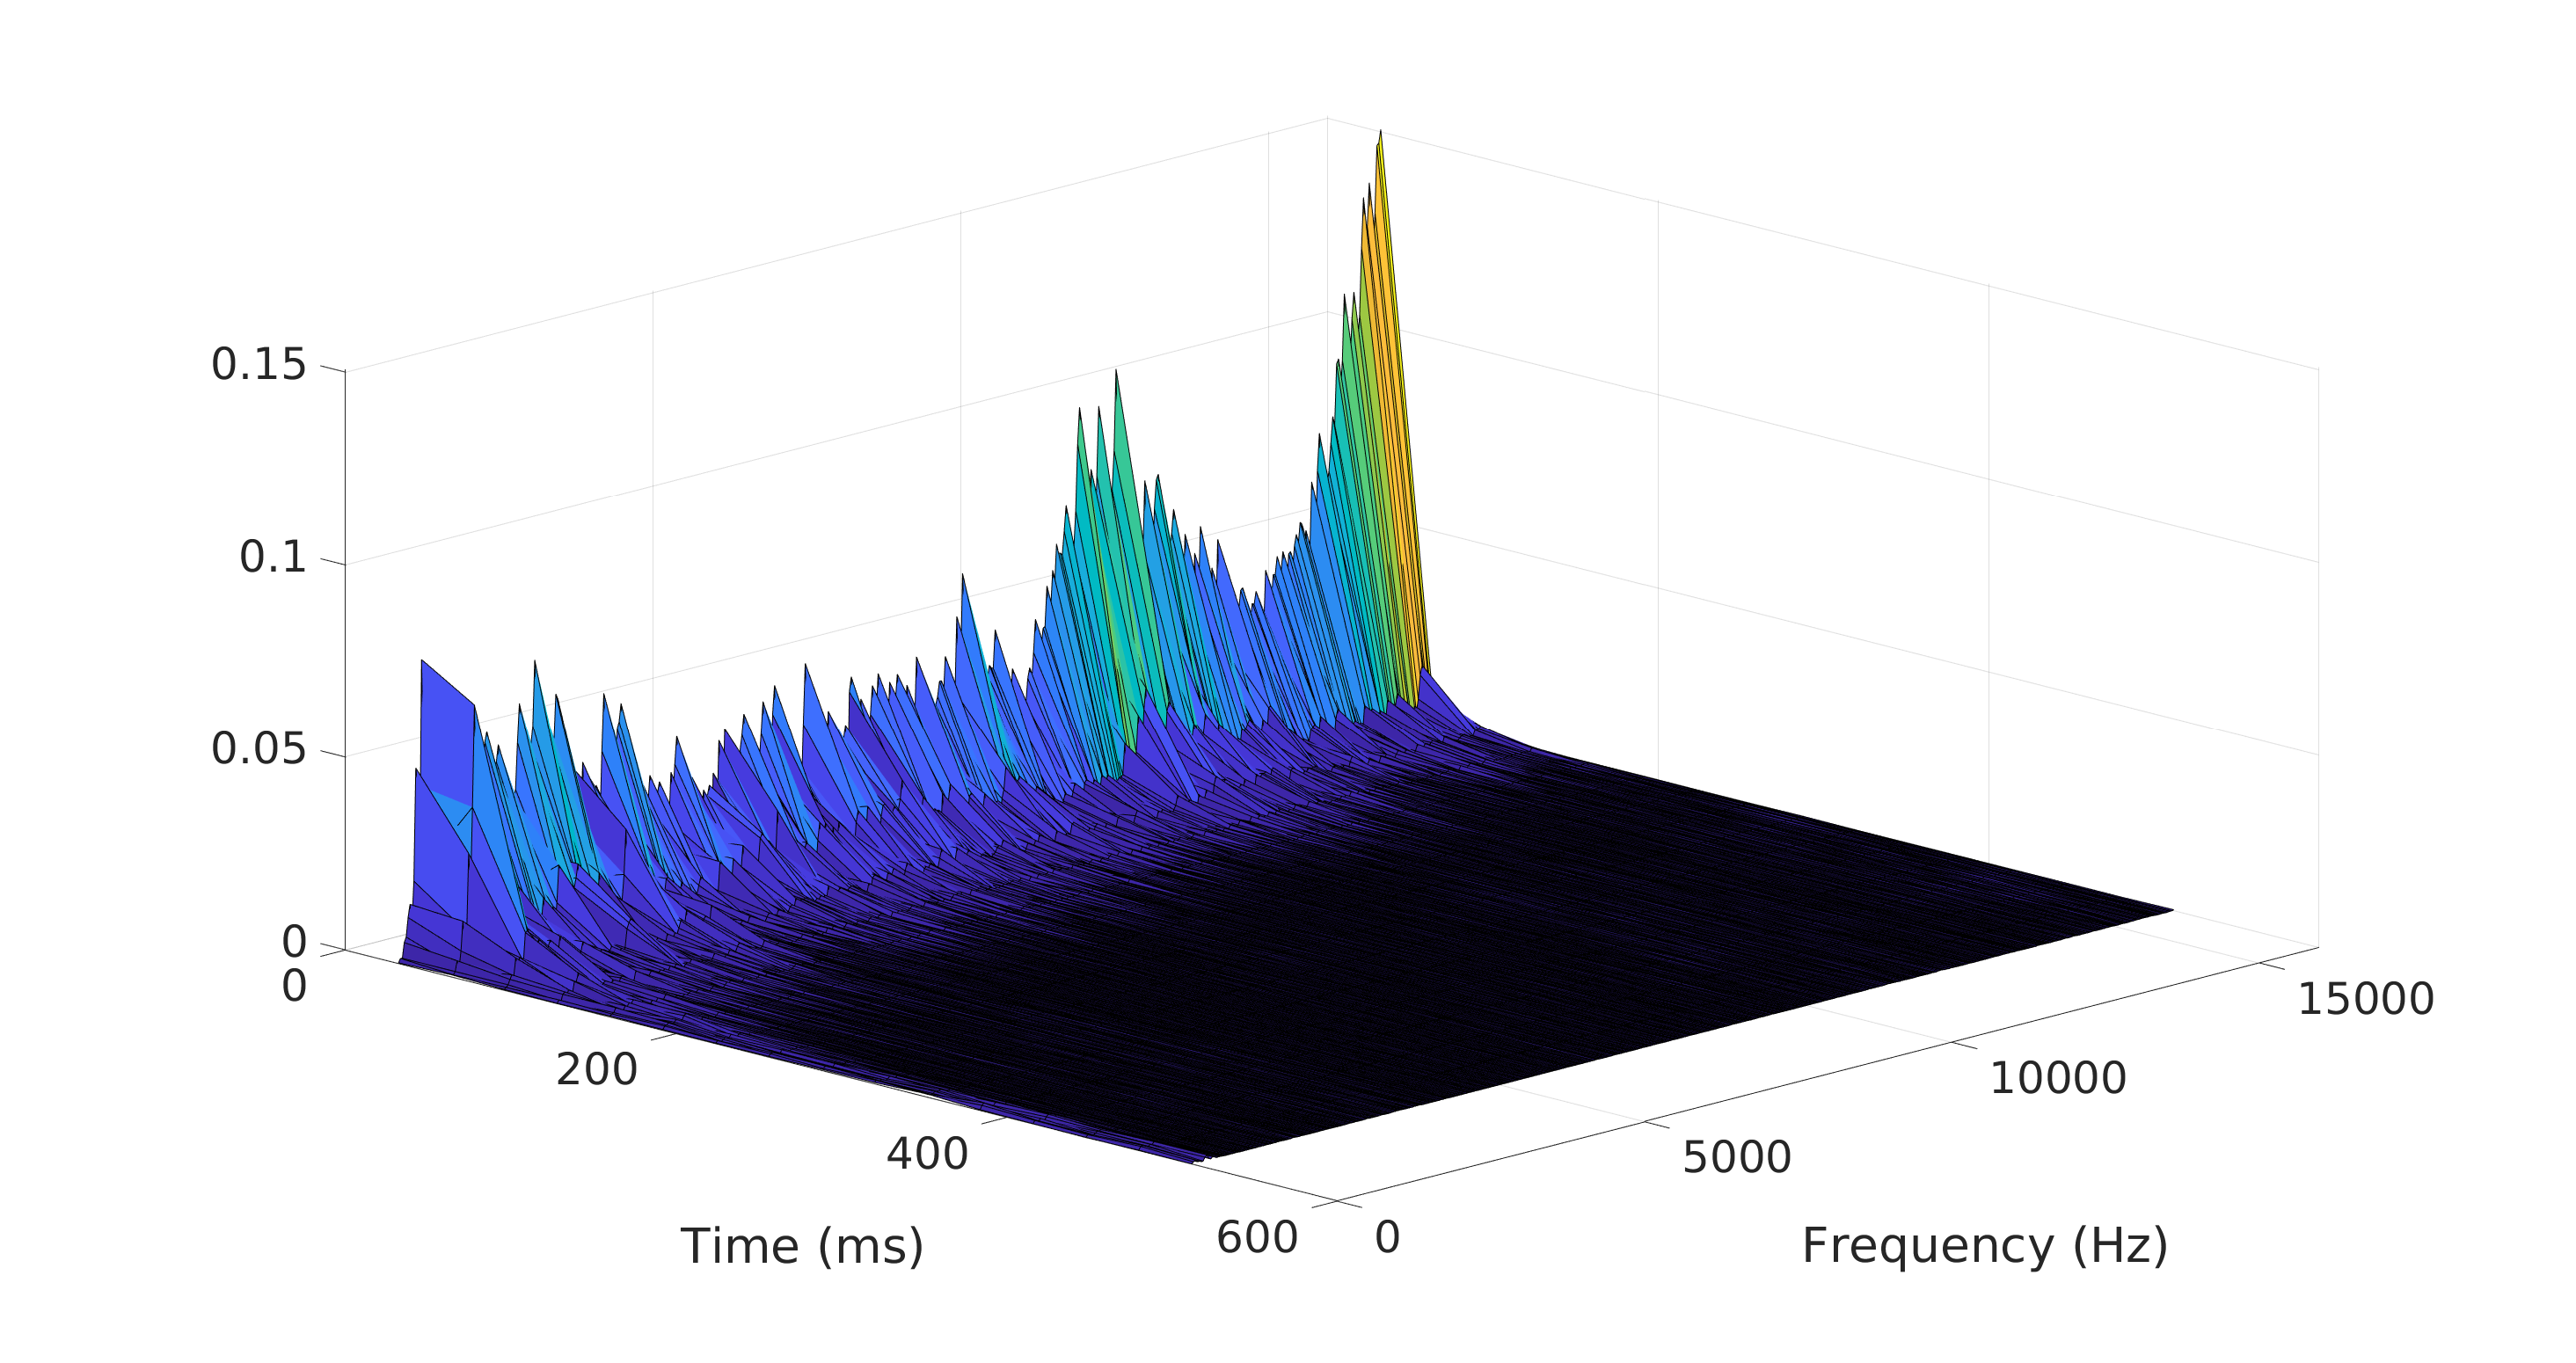
\includegraphics[width=\linewidth]{fig/RIR_original.eps}
\caption{RIR spectrogram obtained for a measured RIR. The RIR has an approximate $T_{60}$ of $500$~ms and source-to-microphone distance (d) of $0.5$~m.}
\label{fig:RIR_spectrogram}
\end{figure}
\fi

\subsection{Spectrogram structure of RIR}
This section details the time-frequency structure present in RIR magnitude spectrogram. The results of the analysis was shown for a particular RIR. However, a similar observations were obtained for other RIRs. 

\subsubsection{Spectral and temporal variations}
This section discusses the frequency envelope and temporal variation of an RIR magnitude spectrogram. The frequency envelope is represented as the spectrum of the frame of RIR having maximum energy. The temporal envelope for a frequency bin $k=\kappa$ represents the variation of RIR spectrogram with time $n$ for a fixed frequency bin i.e, $H(\kappa, n)\text{, }n\in\{0,1,...(L_h-1)\}$.

Figure~\ref{fig:RIR_spectrogram} represents the frequency envelope and temporal variation for different frequency bands for a measured RIR is shown. The RIR has a $T_{60}\approx 700$~ms and a source-microphone distance of $2$~m. It is obtained from REVERB challenge RIR~\cite{kinoshita2016summary}.  Most of the energy in the temporal envelope is concentrated in the initial few frames. The temporal envelope for different frequency bands is shown to decay with time. The decay rate changes with frequency. However, the decays are not strictly exponential as predicted in Pollack's model in Section~\ref{sec:Pollacks_model}. But the model gives a good insight into the time-frequency structure of the magnitude spectrogram of RIR.
\begin{figure}
\centering
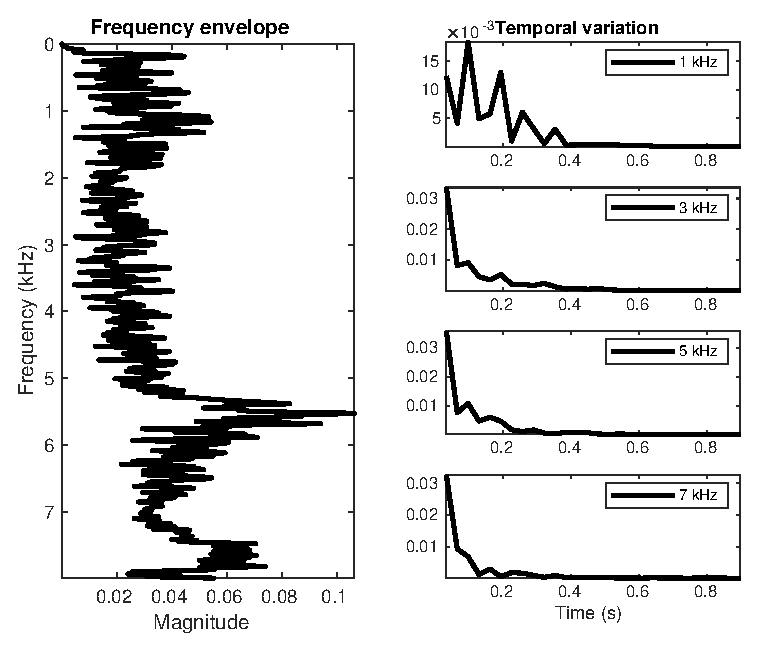
\includegraphics[width = \linewidth]{fig/RIR_Rank1_Original.eps}
\caption{The magnitude spectrogram (left) and temporal envelope for different frequency bands (right) for a measured RIR with $T_{60}\approx700$~ms and source-microphone distance of $2$~m. The temporal envelope decays down with time as is the case in Pollack's model. }
\label{fig:RIR_spectrogram}
\end{figure}

\subsubsection{Sparsity}
Figure~\ref{fig:RIR_spectrogram} shows the spectral envelope and temporal variation of a measured RIR.  It is observed that for all frequency bands, most of the high energy regions occur during the initial few frames after the direct path and dies down to zero after a few frames. This results in the RIR spectrogram having near-zero values for the later frames. In other words, it can be said that the RIR spectrogram is sparse. 

\subsubsection{Separability assumption}
\label{sec:Separability_assumption}
As explained earlier sections, the RIR specrtogram has frequency and time structures. One of the most simplest approach is to treat the temporal and spectral variations independently~\cite{mohanan201a}. The RIR spectrogram $\mathbf{H}$ can be represented with a frequency envelope $H_1(k)$ and temporal variation $H_2(n)$. Mathematically,
\begin{align}
H(k,n) &\approx H_1(k)H_2(n) \text{,}
\end{align}
A rank-$1$ NMF decomposition is performed on the RIR magnitude spectrogram $\mathbf{H}$ to obtain an estimate for $H_1(k)$ and $H_2(n)$. NMF is an iterative algorithm based on a cost function~\cite{lee99}. The cost function is used to measure the correctness of the RIR magnitude spectrogram estimate with the original RIR magnitude spectrogram. In this work, generalized Kullback-Leibler (KL) divergence is used as the cost function. The cost function is represented as,   
\begin{align}
C_{SA} &= \sum_{k = 0}^{K-1}\sum_{n=0}^{L_h-1}\text{KL} (H(k,n)|\hat{H}_{sep}(k,n)) \nonumber \\
\text{KL}(u|v) &= u\text{ln}(\dfrac{u}{v}) + v - u,
\label{eq:KLdiv}
\end{align} 
where $\hat{H}_{sep}(k,n)=H_1(k)H_2(n)$ represents the rank-$1$ approximation of the RIR spectrogram.  A rank-$1$ approximation for the Pollacks model shown in (\ref{eq:PollackModel}) can be obtained by assuming $T_{60}$ is independent of frequency. For this case, $H_1(k) = P(k)$ and $H_2(n)=e^{-\beta n}$.

Figure~\ref{fig:RIR_rank_1_spectrogram} compares the frequency envelope and temporal variation of rank-$1$ approximated RIR spectrogram with the original RIR magnitude spectrogram. It can be observed that most variations of frequency envelope are captured using rank-$1$ approximated  RIR spectrogram. However, the approximation of temporal variations does not capture most of the variations. The main reason for this that the temporal variation changes with frequency band $\kappa$. However, in rank-$1$ approximated RIR magnitude spectrogram model the temporal variation is the same except for a scaling factor of $H_1(\kappa)$. This can pose a limitation in accurately representing the RIR spectrogram.   

\begin{figure*}[ht]
\begin{tabular}{cc}
\subfloat[]{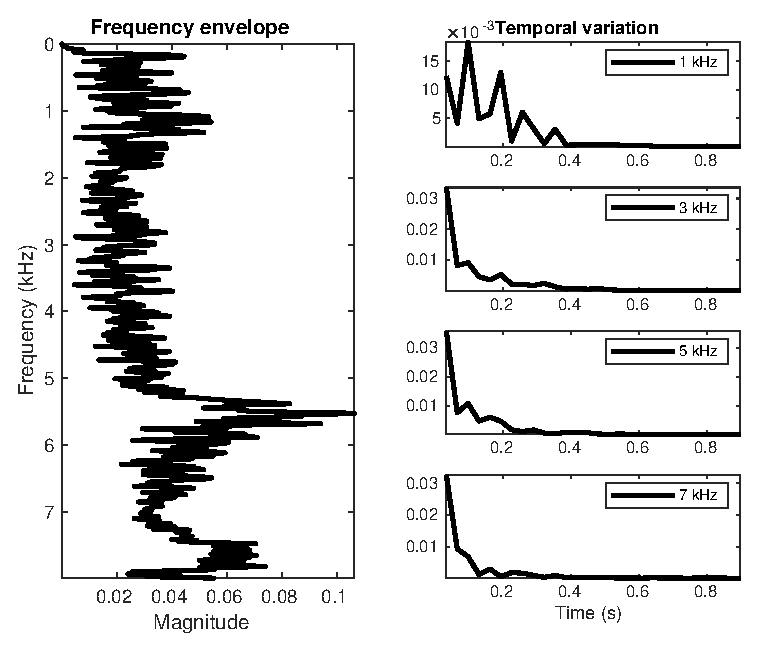
\includegraphics[width = 0.5\linewidth]{fig/RIR_Rank1_Original.eps}} &
\subfloat[]{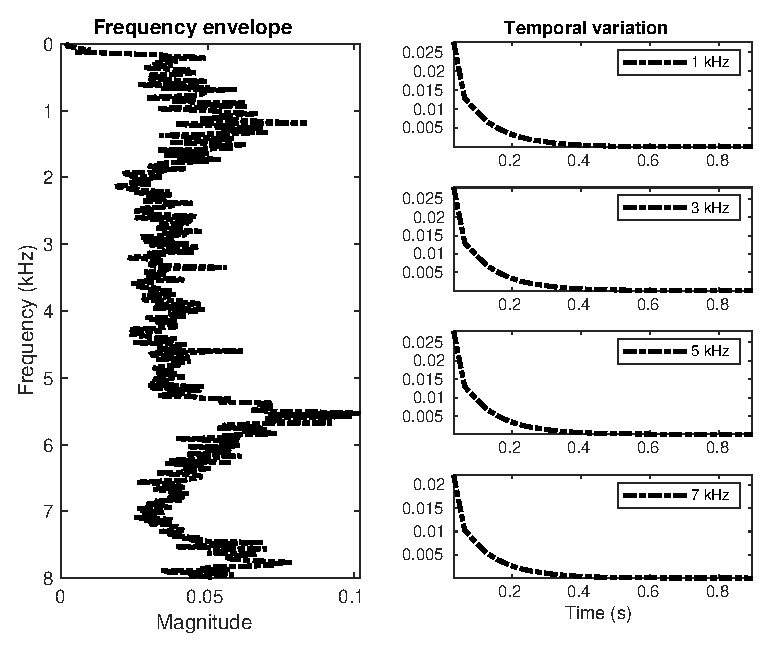
\includegraphics[width = 0.5\linewidth]{fig/RIR_Rank1_Approx.eps}}\\
\end{tabular}
\caption{(a) Frequency envelope and temporal variation obtained for a measured RIR from~\cite{kinoshita2016summary} with $T_{60}\approx 700$~ms and source-to-microphone distance $d=2$~m. (b) Frequency envelope and temporal variation obtained by a rank-$1$ NMF decomposition of the RIR. Frequency envelope approximated in (b) captures the most variations in (a).}
\label{fig:RIR_rank_1_spectrogram}
\end{figure*}
%Such an approximation is a very crude representation of RIR magnitude spectrogram. In this model the temporal variations $H_2(n)$ is assumed to be independent of frequency $k$. One of the imitations of this model is it cannot model the frequency dependency of $T_{60}$. 

\subsubsection{Low-rank nature}
As discussed in Section~\ref{sec:Separability_assumption}, the separability approximation for the RIR magnitude spectrogram is inaccurate. A low-rank approximation is a better model. Based on the low-rank approximation, RIR magnitude spectrogram $\mathbf{H}$ can be represented as,
\begin{align}
\mathbf{H} &\approx \mathbf{H}_1\mathbf{H}_2 \text{,}
\end{align}
where, $\mathbf{H}_1 \in \mathbb{R}_+^{K \times P}$ and $\mathbf{H}_2 \in \mathbb{R}_+^{P \times L_h}$ represents the bases and activation matrix for the NMF decomposition, respectively. $P$ represents the rank of NMF decomposition. Low-rank approximation results in reducing the number of parameters used to represent the RIR spectrogram from $KL_h$ to $P(K+L_h)$~\footnote{$P$ in this case is selected such that $P<L_h$ and $P<<K$}.
$\mathbf{H}_1$ contains $P$ set of frequency envelopes $\mathbf{H}_1^{(p)}\in \mathbb{R}_+^{K \times 1} \text{, } p\in \{1,2,...,P \}$ and $\mathbf{H}_2$ contains the corresponding $P$ set temporal variations $\mathbf{H}_2^{(p)}\in \mathbb{R}_+^{1 \times L_h} \text{, } p\in \{1,2,...,P \}$. Mathematically,
\begin{align}
\mathbf{H}_1 &= \bigg[\mathbf{H}_1^{(1)}\bigg|\mathbf{H}_1^{(2)}\bigg|...\bigg|\mathbf{H}_1^{(P)}\bigg] \nonumber \\
\mathbf{H}_2 &= \bigg[\mathbf{H}_2^{(1)^T}\bigg|\mathbf{H}_2^{(2)^T}\bigg|...\bigg|\mathbf{H}_2^{(P)^T} \bigg]^T
\end{align}
$\mathbf{H}_1$ and $\mathbf{H}_2$ are obtained by performing a NMF decomposition on RIR magnitude spectrogram $\mathbf{H}$.

There exist different approaches to obtain a low-rank approximation. However, the use of NMF decomposition is preferred for the following reason. It ensures that the low-rank approximated RIR spectrogram is non-negative. This is a necessary condition for using a low-rank model in reverberation model discussed in Section~\ref{sec:NMF_methods}. Further, imposing the non-negative constraint on $\mathbf{H}_1$ and $\mathbf{H}_2$ does not compromise on the quality of the estimates as discussed next. 

The cost function used for the purpose has structure similar to (\ref{eq:KLdiv}). The cost function $C_H$ for the purpose can be written as,
\begin{align}
C_{H} &= \sum_{k = 0}^{K-1}\sum_{n=0}^{L_h-1}\text{KL} (H(k,n)|\hat{H}_{rank-P}(k,n)) \nonumber \\
\hat{H}_{rank-P}(k,n) &= \sum_{p=1}^P H_1^{(p)}(k) H_2^{(p)}(n)
\end{align}
where $\hat{H}(k,n)$ is the  (k,n)-th element of the low-rank approximated RIR spectrogram. $H_1^{(p)}(k)$ and $H_2^{(p)}(n)$ represents the elements of $\mathbf{H}_1^{(p)}$ and $\mathbf{H}_2^{(p)}$, respectively.


\iffalse
Experimentally it can be shown that the low-rank approximated RIR spectrogram $\mathbf{\hat{H}}$ is a good approximation for the original RIR spectrogram. A low-rank RIR spectrogram is obtained using a multiplicative algorithm proposed in~\cite{lee99}. It uses Generalized Kullback-Leibler (KL) divergence as the cost function. The cost function used in the work are summarized as,
\begin{align}
C_{rank-P} &= \sum_{k = 0}^{K-1}\sum_{n=0}^{L_h-1}\text{KL} (H(k,n)|\hat{H}(k,n)) \nonumber \\
\text{KL}(u|v) &= u\text{log}(\dfrac{u}{v}) + v - u,
\label{eq:KLdiv1}
\end{align} 
where $\hat{H}(k,n)$ is the  (k,n)-th element of the low-rank approximated RIR spectrogram.
\fi
 
$C_{H}$ captures the net deviation occurred due to the low-rank approximation of the RIR spectrogram. The deviation $C_{H}$ depends on the rank-$P$ of the decomposition. Figure~\ref{fig:cost_rank_P_approximation} analyses this dependency for different measured RIR available from~\cite{kinoshita2016summary}. The figure shows the mean and extreme variation for $C_{H}$ with $P$. It is observed that deviation reduces with increasing $P$, and variation saturates after $P=10$ indicating that a rank-$P$ approximation is sufficient for the purpose. 
Figure~\ref{fig:RIR_rank_P_spectrogram} compares the original frequency envelope and temporal variation of a RIR with the one obtained using a rank-$10$ NMF decomposition. The frequency envelope and temporal variation present in the original RIR magnitude spectrogram is accurately captured using a rank-$10$ approximation.
\begin{figure}[ht]
\centering
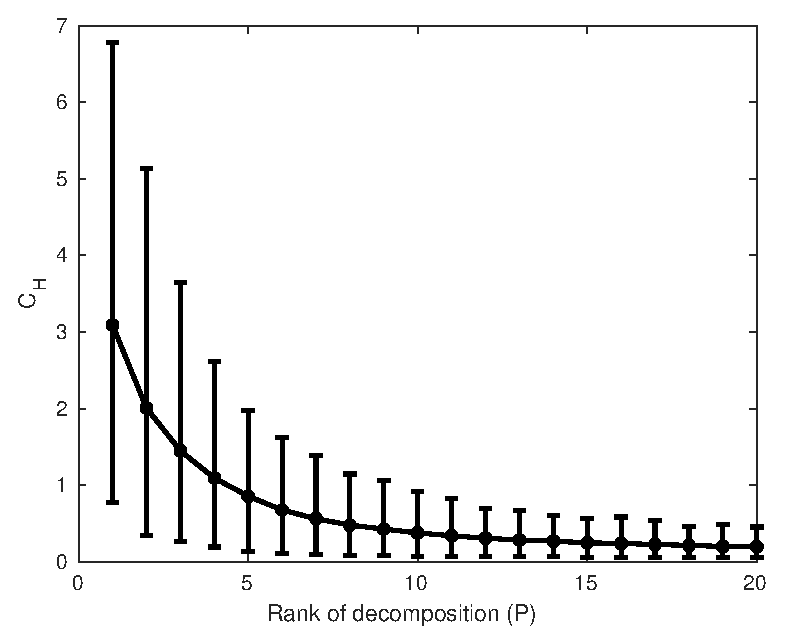
\includegraphics[width=\linewidth]{fig/RIR_NMF_approx_cost_error_plot.eps}
\caption{Effect of varying rank $P$ on the low-rank approximation for the RIR spectrogram. The deviation from the original RIR spectrogram reduces with increasing $P$. The deviation is small for $P>10$.}
\label{fig:cost_rank_P_approximation}
\end{figure}

\begin{figure*}[ht]
\begin{tabular}{cc}
\subfloat[]{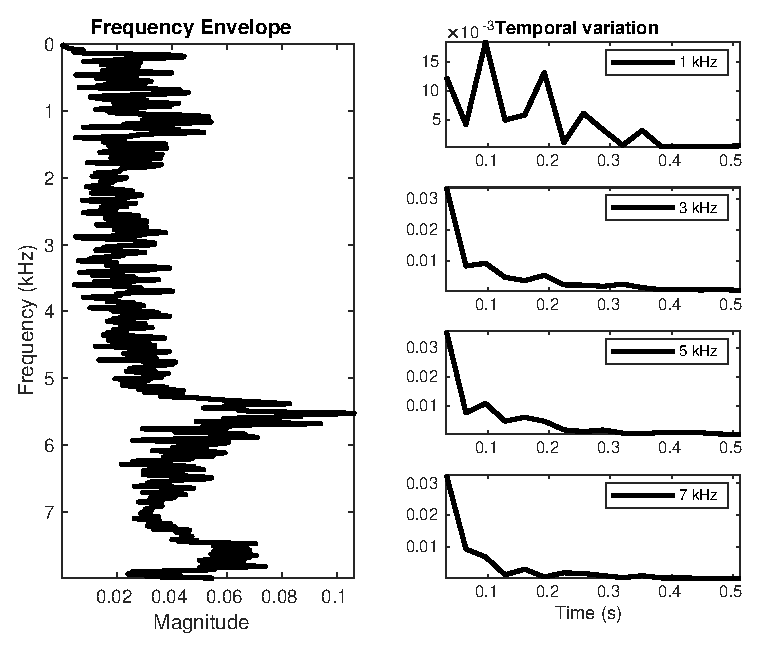
\includegraphics[width = 0.5\linewidth]{fig/RIR_NMF_far_original.eps}} &
\subfloat[]{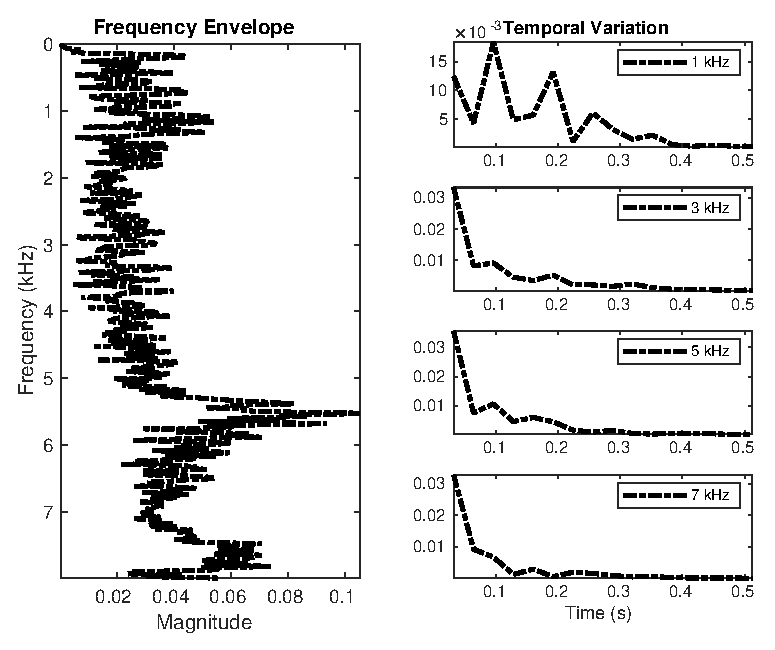
\includegraphics[width = 0.5\linewidth]{fig/RIR_NMF_far_approx.eps}}\\
\end{tabular}
\caption{(a) Frequency envelope and temporal variation obtained for a measured RIR from~\cite{kinoshita2016summary}. (b) Frequency envelope and temporal variation obtained by a rank-$10$ NMF decomposition of the RIR. (b) is a very good approximation of (a).}
\label{fig:RIR_rank_P_spectrogram}
\end{figure*}

\iffalse
\begin{figure*}[ht]
\begin{tabular}{cccc}
\subfloat[]{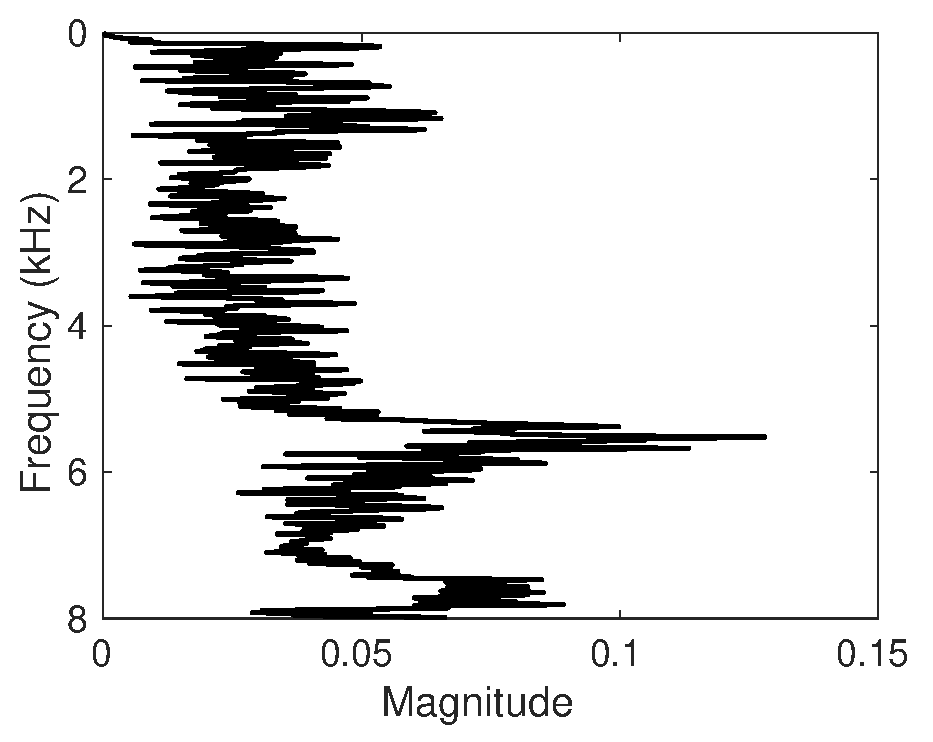
\includegraphics[width = 0.25\linewidth]{fig/RIR_env_original_RIR_cond_RIR_SimRoom3_far_AnglA_StationaryNoise_10dB.eps}} &
\subfloat[]{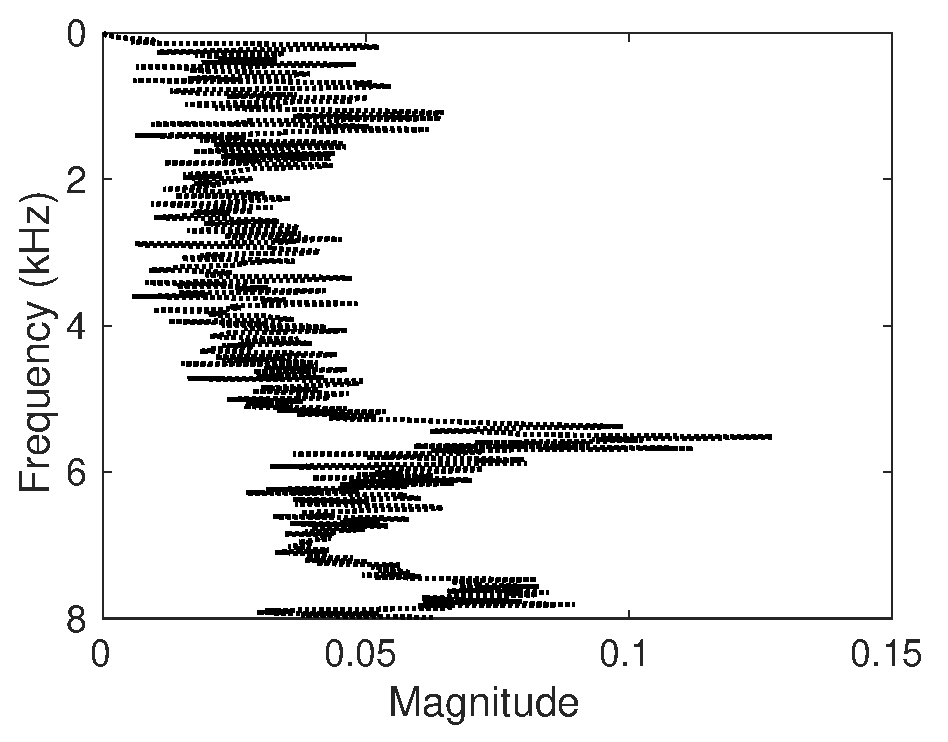
\includegraphics[width = 0.25\linewidth]{fig/RIR_env_approx_RIR_cond_RIR_SimRoom3_far_AnglA_StationaryNoise_10dB.eps}} &
\subfloat[]{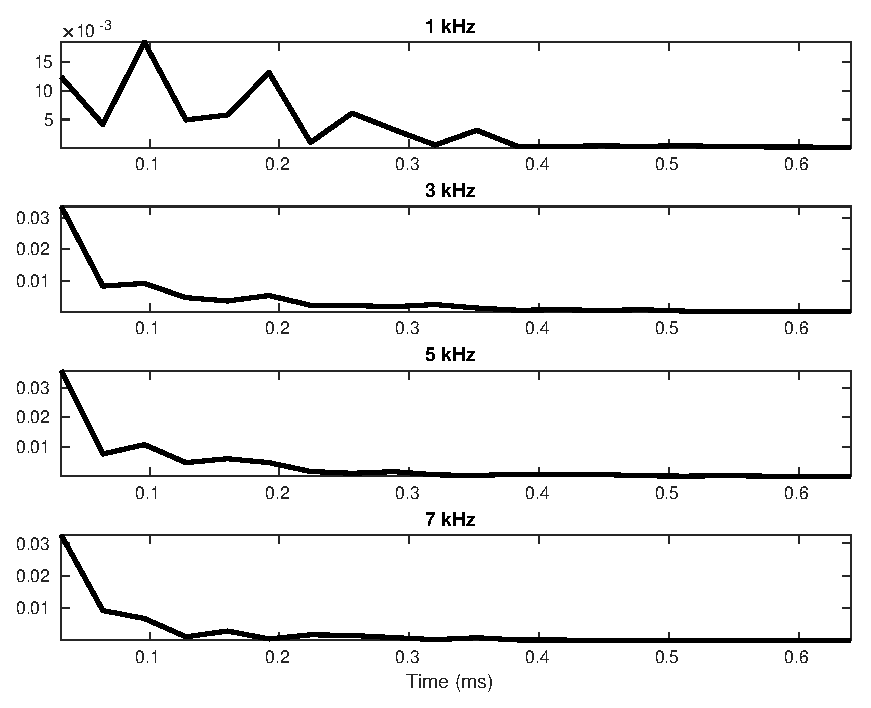
\includegraphics[width = 0.25\linewidth]{fig/RIR_tempo_original_RIR_cond_RIR_SimRoom3_far_AnglA_StationaryNoise_10dB.eps}} &
\subfloat[]{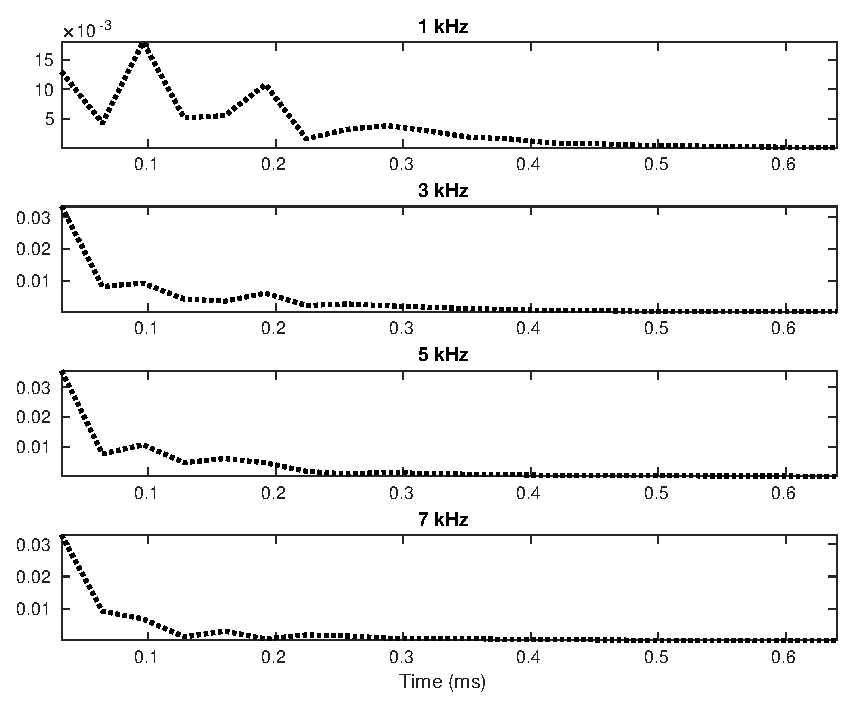
\includegraphics[width = 0.25\linewidth]{fig/RIR_tempo_approx_RIR_cond_RIR_SimRoom3_far_AnglA_StationaryNoise_10dB.eps}} \\
\end{tabular}
\caption[abc]{(a) Frequency envelope and temporal variation for different bands for the spectrogram obtained for a measured RIR from~\cite{kinoshita2016summary} having an approximate $T_{60}$ of $500$~ms and source-to-microphone distance (d) of $2$~m. (b) Frequency envelope and temporal variation obtained by a rank-$10$ NMF decomposition of the RIR. (b) is a very good approximation of (a).}
\label{fig:RIR_rank_P_spectrogram}
\end{figure*}
\fi

\section{Characteristics of RIR}
This Section details the various parameters associated with a RIR. 

\subsection{Source-microphone distance ($d_{sd}$)}
The structure of RIR changes with the position of microphone and source, especially the source-microphone distance ($d_{sm}$). The direct-path energy decreases with an increase in $d_{sm}$, whereas the diffused nature of reverberation results in the reverberant energy remaining mostly constant~\cite{naylor2010speech}. As a result, the effects due to the reverberation tail becomes more prominent with increasing distance.

\subsection{Reverberation time ($T_{60}$)}
When a sound source placed in a reverberant room is switched off, it takes a finite time for the sound level to decay down. The $T_{60}$ is defined as the time taken for the sound level to drop $60$~dB below the level at sound cessation~\cite{ratnam2003blind}. $T_{60}$ is fixed of a reverberant room. Typically, $T_{60}$ varies with properties of the room like absorption coefficients of the wall, etc and is independent of the position of source and microphone~\cite{naylor2010speech}. Reverberation time changes with frequency~\cite{jeub2010we}, but it is typically represented by a single value which indicates the dominant mode~\cite{naylor2010speech}.  

\subsection{Direct-to-reverberation ratio (DRR)}
DRR is defined as the ratio of energy present in the direct-path and early reflections of the RIR to the total energy present in the RIR~\cite{kinoshita2016summary}. The reflections delayed upto  $50$~ms from the direct-path forms the early part. Mathematically,
\begin{align}
DRR &= \dfrac{\sum_{n=0}^{n_e}h^2(n)}{\sum_{n=n_e+1}^{L_h} h^2(n)} \nonumber \\
\dfrac{n_e}{f_s}  &= 50\times 10^{-3} \text{s,}
\end{align} 
where $n_e$ represents the number of samples used to represent the early part of RIR. $f_s$ represents the sampling frequency. DRR gives a measure of the contribution of coloration occurring due to the early part of RIR to the net effects of reverberation. DRR varies with $d_{sm}$ and $T_{60}$~\cite{naylor2010speech}.

\section{Conclusion}
This chapter discussed the various time and frequency domain structure present in RIR. The disadvantage of using single-channel inverse filtering approaches was discussed next. Finally, different structures present in the magnitude spectrogram of RIR is discussed. The following chapters will utilize these RIR spectrogram structures in the speech enhancement algorithms.


\chapter{Dereverberation based on RIR constrained cost function}
\label{chapter:icassp2017}

This chapter explains NMF based dereverberation methods that utilize three different properties of RIR spectrogram - sparsity, frequency envelope, and early part of RIR. Such methods are derived by modifying the basic NMF based dereverberation methods available in the literature. The initial section of this chapter explains the basic NMF based dereverberation problems. Later part of the chapter explains the modifications made to accommodate the above mentioned RIR properties in the dereverberation problem. This discussion is followed by the analysis of enhancement results. 

\section{Basic NMF based dereverberation methods}
\label{sec:basic_NMF_reverb_model}
This section explains the approach taken to estimate clean speech and RIR spectrogram based on the basic reverberation models discussed in Section~\ref{sec:NMF_methods}. The algorithms based on the CNMF reverberation model in (\ref{eq:cnmf0}) and CNMF reverberation model with NMF clean speech model in (\ref{eq:cnmf1}) is discussed next. 

\subsection{CNMF based reverberation model}
The CNMF model for reverberated speech spectrogram was discussed in Section~\ref{sec:NMF_methods}. In~(\ref{eq:cnmf0}), the reverberated speech spectrogram $Y_R\in\mathbb{R}_+^{K \times T}$ is approximated as convolution of clean speech spectrogram $\mathbf{S}\in\mathbb{R}_+^{K \times (T-L_h+1)}$ and RIR spectrogram $\mathbf{H}\in\mathbb{R}_+^{K \times L_h}$. 
\begin{equation}
Y_R(k,n)\approx \sum_{l=0}^{L_h-1} H(k,l)S(k,n-l),
\label{eq:cnmf0_1}
\end{equation}
where $Y_R(k,n)\text{, } H(k,n) \text{ and }S(k,n)$ represents the elements of $\mathbf{Y_R}\text{, } \mathbf{H} \text{ and }\mathbf{S}$, respectively.
Iterating algorithm was proposed for solving for $S(k,n)$ and $H(k,n)$ based on reverberation model in (\ref{eq:cnmf0_1})~\cite{kameoka2009robust,Kumar2011}. The parameters are estimated such that it minimizes a cost function. Euclidean distance (ED)~\cite{kameoka2009robust} and generalized KL divergence~\cite{Kumar2011} are commonly used cost functions. Generalized KL divergence (KL) as cost functions gives reduced modeling error when compared to ED. The optimization problem for solving the CNMF based reverberation model based on KL divergence can be written as,
\begin{align}
&C_{cnmf0} = \underset{S(k,n)\text{, }H(k,n)}{\text{argmin}} \Bigg[ \sum_{k,n} \text{KL} \bigg(Y_R(k,n)|\tilde{Y}_R(k,n)\bigg)+\lambda_{cnmf0}\sum_{k,n}S(k,n) \Bigg] \nonumber \\ 
\text{Subjected to}& \nonumber \\
&H(k,n) \geq 0\text{, }S(k,n)\geq 0 \nonumber \\ 
&\sum_{n}H(k,n) = 1 \text{,}
\label{eq:cost_cnmf0}
\end{align}
where $\tilde{Y}_R(k,n)$ represents the estimated reverberated spectrogram based on (\ref{eq:cnmf0_1}). $\lambda_{cnmf0}$ is a weighting factor. The cost function in (\ref{eq:cost_cnmf0}) has two terms. First term is a measure of deviation between actual and estimated reverberated speech spectrogram. The second term introduces sparsity to the estimated clean speech spectogram. The amount of sparsity is controled by $\lambda_{cnmf0}$. It is fixed as $\lambda_{cnmf0}=\dfrac{10^{-8}}{KT}\sum\limits_{k,n}Y_R(k,n)$. This first set of constraints make sure that the estimated $S(k,n)$ and $H(k,n)$ are non-negative. This is necessary as these terms represents magnitude spectrograms. The normalization $\sum\limits_{n}H(k,n) = 1$ was required to avoid scaling ambiguity and the subsequent estimation of undesired solution~\footnote{Assume a clean speech spectrogram $S(k,n)$ and RIR $H(k,n)$ minimizes the first term in (\ref{eq:cnmf0_1}). Then $aS(k,n)\text{, }a\in \mathbb{R}_+$ and $H(k,n)/a$ will also minimizes the first term. So, the cost function (\ref{eq:cnmf0_1}) is minimized by the value that minimizes the second term. This happens when $S(k,n)=0$, resulting in $H(k,n)=\infty$.}. Iterative algorithm based on a multiplicative update rule was proposed to find the solution~\cite{Kumar2011}. The update rule for the parameters are shown in (\ref{eq:multi_update_cnmf0}). This method is referred to as CNMF0.
\begin{align}
H(k,n) & \leftarrow H(k,n) \dfrac{\sum\limits_l\dfrac{Y_R(k,l)}{\tilde{Y}_R(k,l)}S(k,n-l)}{\sum\limits_l S(k,n-l) } \nonumber \\
S(k,n) & \leftarrow S(k,n)\dfrac{\sum\limits_l\dfrac{Y_R(k,l)}{\tilde{Y}_R(k,l)}H(k,n-l)}{\sum\limits_l H(k,n-l) + \lambda_{cnmf0}} 
\label{eq:multi_update_cnmf0}
\end{align}

The steps involved in CNMF0 is summarized in Algorithm~\ref{algo:cnmf0}. The time-domain de-reverberated speech is obtained by performing an inverse STFT on the complex spectrogram of the estimated clean speech. The complex spectrogram is constructed by using the phase spectrogram obtained from the reverberated speech along with the enhanced magnitude spectrogram.  
% spectrogram comparison plots

%\iffalse
\begin{algorithm}[H]
\SetAlgoLined
\KwResult{ Enhanced speech spectrogram $S(k,n)$ }
 initialize $S(k,n)$, $H(k,n)$ to random positive values\;
  \For{$i=1:\text{i\_max}$}{
    update $S(k,n)$\\
    update $H(k,n)$\\
    normalization $H(k,n) \leftarrow \dfrac{H(k,n)}{\sum\limits_n H(k,n)}$
    }
 \caption{Steps involved in CNMF0}
 \label{algo:cnmf0}
\end{algorithm}
%\fi
\subsection{CNMF model with NMF model for clean speech}
The CNMF reverberation model was modified by incorporating a model for clean speech. The clean speech spectrogram was approximated using a NMF model as, 
\begin{align}
\mathbf{S}&\approx \mathbf{W}_s\mathbf{X}_s \nonumber \\
S(k,n)&\approx \sum\limits_{r=1}^{R_s} W_s(k,r)X_s(r,n),
\end{align}
where $\mathbf{W}_s\in\mathbb{R}_+^{K\times R_s}$ and $\mathbf{X}_s\in\mathbb{R}_+^{R_s\times (T-L_h+1)}$ represents the bases and activation matrix. $R_s$ represents the rank of NMF decomposition. $W_s(k,r)$ and $X_s(r,n)$ are elements of $\mathbf{W}_s$ and $\mathbf{X}_s$, respectively. Utilizing the NMF model in (\ref{eq:cnmf0_1}), the reverberation model can be rewritten as,
\begin{equation}
Y_R(k,n)\approx \sum\limits_{l=0}^{L_h} H(k,l)\bigg[\sum\limits_{r=1}^{R_s}W_s(k,r)X_s(r,n-l)\bigg]
\label{eq:cnmf1_1}
\end{equation}
An algorithm was proposed to obtain clean speech and RIR spectrograms from reverberation model in (\ref{eq:cnmf1_1})~\cite{mohammadiha2016speech, Mohammadiha2015}. The optimization problem can be summarized as,
\begin{align}
&C_{cnmf1} = \underset{\mathbf{H}\text{, }\mathbf{W}_s\text{, }\mathbf{X}_s}{\text{argmin}} \Bigg[ \sum_{k,n} \text{KL} \bigg(Y_R(k,n)|\tilde{Y}_R(k,n)\bigg)+\lambda_{cnmf1}\sum_{r,n}X_s(r,n) \Bigg] \nonumber \\ 
\text{Subjected to}& \nonumber \\
&H(k,n) \geq 0\text{, }W_s(k,r)\geq 0\text{, }X_s(r,n)\geq 0 \nonumber \\ 
&H(k,0) = 1\forall k\in \{0,1,...,(K-1)\} \text{,}
\label{eq:cost_cnmf1}
\end{align}
where $\tilde{Y}_R(k,n)$ represents the estimated reverberated spectrogram based on reverberation model in (\ref{eq:cnmf1_1}). $\lambda_{cnmf1}$ represents a weighting factor. The objective function has two terms. The first term minimizes the modeling error between estimated and actual reverberated speech spectrograms. The second term introduces sparsity in estimated clean speech activation. The first set of constraints ensures that the estimated clean speech and RIR spectrograms are non-negative. Normalization in the RIR spectrogram removes the inherent scaling ambiguity present in the cost function.

Multiplicative update rule was obtained for solving the optimization problem in (\ref{eq:cost_cnmf1})~\cite{mohammadiha2016speech, Mohammadiha2015}. The update rules are summarized in (\ref{eq:multi_update_cnmf1}).
\begin{align}
H(k,n) & \leftarrow H(k,n) \dfrac{\sum\limits_l\dfrac{Y_R(k,l)}{\tilde{Y}_R(k,l)}S(k,n-l)}{\sum\limits_l S(k,n-l) } \nonumber \\
W_s(k,r) & \leftarrow W_s(k,r) \dfrac{\sum\limits_{n,l}\dfrac{Y_R(k,n)}{\tilde{Y}_R(k,n)} H(k,l)X_s(r,n-l)}{\sum\limits_{n,l} H(k,l)X_s(r,n-l)} \nonumber \\
X_s(r,n) & \leftarrow X_s(k,r) \dfrac{\sum\limits_{k,l}\dfrac{Y_R(k,l)}{\tilde{Y}_R(k,l)} H(k,n-l)W_s(k,r)}{\sum\limits_{k,l} H(k,n-l)W_s(k,r)+\lambda_{cnmf1}}
\label{eq:multi_update_cnmf1}
\end{align}
where $\tilde{S}(k,n)=\sum\limits_r W_s(k,r)X_s(r,n)$.
There exists two approaches. This distinction is based on how $W_s(k,r)$ is estimated. In unsupervised (offline) approach, the clean speech bases $W_s(k,r)$ is estimated from the reverberated data. This approach is referred to as \text{CNMF1\_u}. In supervised (online) approach, $W_s(k,r)$ are pre-learned. A NMF decomposition is performed on the spectrogram of available clean speech recording. The bases vectors obtained for this decomposition forms $W_s(k,r)$. This method is referred to as \text{CNMF\_s}. The steps involved are summarized in Algorithm~\ref{algo:cnmf1}. 

\begin{algorithm}[H]
\SetAlgoLined
\KwResult{ Enhanced speech spectrogram $S(k,n)$ }
 initialize $W_s(k,r)$, $X_s(r,n)$, $H(k,n)$ to random positive values\;
  \For{$i=1:\text{i\_max}$}{
     \If{$W_s(k,r)$ is not fixed}{
      update $W_s(k,r)$\\
      }
    update $X_s(r,n)$\\
    update $H(k,n)$\\
     \If{$H(k,n)>H(k,n-1)$}{
      truncation of $H(k,n)$ \\ 
      $H(k,n)\leftarrow \text{min}\bigg( H(k,n), H(k,n-1) \bigg)$\\
      }    
    normalization $H(k,n) \leftarrow \dfrac{H(k,n)}{ H(k,0)}$
    }
  estimation of clean speech spectrogram 
  $S(k,n)=\dfrac{\sum\limits_{r=1}^{R_s} W_s(k,r)X_s(r,n)}{\tilde{Y}_R(k,n)}Y_R(k,n)$
 \caption{Steps involved in \text{CNMF1\_s and CNMF1\_u} }
 \label{algo:cnmf1}
\end{algorithm}

\subsection{Comparison of reverberation models}

\section{Incorporation of RIR properties on optimization problem}
The NMF based dereverberation methods discussed in Section~\ref{sec:basic_NMF_reverb_model} used properties of clean speech spectrogram like low-rank nature and sparsity. However, such methods did not incorporate any properties of RIR except for basic truncation and normalization of the RIR spectrogram. This chapter focuses on incorporating three meaningful constraints on the RIR spectrogram to improve the dereverberation performance of basic NMF based dereverberation methods. The properties of RIR used are (i) frequency envelope of RIR spectrogram, (ii) sparsity of RIR spectrogram, and (iii) retaining the early part of the RIR spectrogram. These approaches are explained in detail next.

\subsection{Frequency envelope of RIR spectrogram}
\subsection{Sparsity of RIR spectrogram}
\subsection{Retaining early part of RIR}

\iffalse
\section{Requirement}
\begin{itemize}
\item NMF based reverberation methods does not use RIR model (except truncation) in cost function
\item Also does normalization on RIR spectrogram 
\item Resulting in sub-optimal performance
\end{itemize}
\section{Proposed approach}
\begin{itemize}
\item introduces constraints on estimated RIR spectrogram in cost function
\item incorporate both speech and RIR model
\item improving speech enhancement results and proper RIR estimates
\item Three appraoches
\begin{itemize}
\item frequency envelope of RIR
\item sparsity on RIR spectrogram
\item retaining early part of RIR
\end{itemize}  
\end{itemize}
\section{Experimental results - enhancement results} 
\section{Discussions} 
\fi

\iffalse
Distant speech enhancement and recognition has been gaining importance over the
past decade due to the prevalence of audio capturing
instruments~\cite{Kumatani2012}. Such
instruments could be mobile phones, voice recorders, microphones in a conference
room or an automobile. Distant speech refers to scenarios where the audio source
and capturing device are separated at least by a feet. Speech processing (for
recognition or enhancement) in such environments differs from traditional speech
processing as it has to compensate for reverberation effects in the captured
data. While speech dereverberation has been an active research area for a long
time~\cite{naylor2010speech}, it has gained interest recently~\cite{reverb2014}
for the reason mentioned above. Speech dereverberation can be done using single-
or multi-channel data depending on the application of interest. The main objective in
this research is to address single-channel dereverberation in the distant speech scenario. The performance is evaluated for both speech enhancement and automatic speech recognition task. 

The effect of reverberation on speech depends not only on the speech signal, but
also on the room or environment under consideration. Reverberation alters speech
in a way much different from other types of environmental noise. The environment
or the room can be modelled as an impulse response or specifically as room
impulse response (RIR). The characteristics of this RIR have a significant
effect on the reverberant signal, and hence a good understanding of this is
relevant for dereverberation. This is more important when addressing this
problem as a blind deconvolution problem. 

Dereverberation methods can be classified as those that (i) cancel reverberation or
(ii) suppress reverberation. The reverberation cancellation methods include blind
deconvolution based methods. The reveberation suppression methods include
spectral substraction, linear prediction (LP) based methods, and statistical
methods for spectral enhancement. Here we consider a non-negative matrix
factorization (NMF) based approach that can be classified as reverberation suppression
approach. This uses the magnitude spectrum of the reverberant signal, and with
minimal prior knowledge of the RIR, to obtain the dereveberated speech signal.
The earliest work to introduce the notion of NMF for
dereverberation~\cite{kameoka2009robust} provides a statistical motivation for use of NMF
to solve the dereverberation problem. More recently there have been several
improvements over the basic NMF based approache for dereverberation in both
single-channel~\cite{Mohammadiha2016, baby2016supervised, Mohammadiha2015, Kallasjoki2014, Kumar2011}, and multi-channel~\cite{Yu2012}, ~\cite{Yu2014}, ~\cite{Mirsamadi2014} scenarios.
In~\cite{Mohammadiha2016, Mohammadiha2015} the initial NMD model for speech
dereverberation is improved by integrating various NMF models for the speech
signal within the original model leading to several NMD-NMF approaches. The work
in~\cite{baby2016supervised} along with a NMD-NMF approach uses a NMF model for external
additive noise and hence does both dereverberation and denoising. Most of
these methods use the short-time Fourier transform (STFT) spectrum representation of the
signal when performing NMF. The method proposed in~\cite{Kumar2011} uses a
gammatone filtered spectrum in the NMF framework and has shown improvements in
word error rates (WER) over the earlier NMF based methods. These methods also
have proposed incorporating a sparsity constraint on the speech signal as a
regularizer to improve speech enhancement. All these approaches
have demonstrated improvement in speech enhancement measures
and or WER improvement. NMF based methods for dereverberation provide an
estimate of the clean speech signal and the corresponding room impulse response
(RIR). While the estimation accuracy of the speech signal is considered in all
existing approaches, they do not provide an evaluation of the accuracy of the
RIR estimate. The single-channel NMF dereverberation problem is treated as a
deconvolution in the sub-band domain. Obtaining the RIR from the observed
reverberant signal is a unconstrained problem and possibly many solutions.
Hence, its required to impose appropriate constraints in obtaining the solution.
Earlier NMF approaches obtained reasonable estimates for speech by imposing a
sparsity constraint or by using appropriate models for speech. The objective in
this work is to consider the RIR estimates and relate them to the expected
estimates, within the reverberation model constraints. Such an analysis is used
further to provide regularizations or constraints on the RIR, leading to better
estimates of both the clean speech signal and RIR of the system. These
constraints are motivated from both time-domain and frequency-domain models of
the revereberant RIR~\cite{naylor2010speech}. The proposed regularization on RIR
will be evaluated using speech enhancement measures such as PESQ, SRMR, and CD. The speech enhancement task is evaluated using improvement in WER.
%These guidelines include complete descriptions of the fonts, spacing, and
%related information for producing your proceedings manuscripts. Please follow
%them and if you have any questions, direct them to Conference Management
%Services, Inc.: Phone +1-979-846-6800 or email
%to \\\texttt{papers@ieee-icassp2017.org}.

\section{NMF based speech dereverberation}
The reverberant speech model considered when using NMF for dereverberation and a
brief description of existing NMF approaches to solve this problem are described
in this section. The goal of NMF algorithms is to factorize a non-negative
matrix $\mat{V} \in \mathbb{R}^{F \times T}$, consisting of elements $v_{i,j} >
0, \forall i,j$, into a product of two non-negative matrices $\mat{W} \in
\mathbb{R}^{F \times R}$ and
$\mat{U} \in \mathbb{R}^{R \times T}$, such that
\begin{equation}
\mat{V} = \mat{W} \mat{U}.
\label{eqn:NMFBasicProduct}
\end{equation}
Here, the columns $w_i\in \mathbb{R}^{F \times 1}, i \in \{1,\ldots, R\}$ of $\mat{W}$ can be considered as a set
of basis vectors and the rows $u_i\in\mathbb{R}^{1 \times T}, i \in \{1, \dots, R\}$ of $\mat{U}$ are the
weights or activations to obtain the columns $v_i, i \in \{1, \ldots, T\}$ of
$\mat{V}$. Efficient algorithms to solve (\ref{eqn:NMFBasicProduct}) using
multiplicative-updates were initially proposed in~\cite{lee99}. Since then NMF
algorithms have been used in several applications. In speech or audio
processing, NMF can be applied if the magnitude spectrum of the signal is
considered as $\mat{V}$. Several variants of NMF have been proposed for source
separation, denoising, and enhancement of speech and music signals. Here, we will restrict our discussion to the use of NMF for speech
enhancement or dereverberation.    

% reverberant speech model
For NMF to be used in speech dereverberation the spectral representation of the
observed or reverberated signal needs to be understood. In time-domain, the observed signal
$x[n]$ in a microphone as result of a clean speech signal $s[n]$ in a
reverberant room with room impulse response (RIR) $h[n]$, can be represented as
\begin{equation}
  x[n] = s[n] * h[n] = \sum_{m=0}^{M-1} h[m] s[n-m],
  \label{eqn:reverb_t}
\end{equation}
where $*$ represents convolution in time-domain, and $M$ is the length
of the RIR. In NMF we require a frequency-domain representation of the signal.
Hence, we are interested either in the short-time Fourier transform (STFT)
representation or any equivalent transform where a representation as
in~(\ref{eqn:NMFBasicProduct}) is possible. Here, we will consider the magnitude of
the STFT spectrum of the signal and follow a representation motivated
in~\cite{kameoka2009robust} and later followed
in~\cite{Kumar2011},~\cite{Mohammadiha2016}.  
One main aspect of this representation is that it handles the reverberant RIRs
which are typically longer (in 100s of ms) compared to the STFT analysis window
duration of 20-40~ms considered in speech analysis. In this STFT model, the STFT
of the reverberated signal is considered as a convolution of the $s[n]$ and
$h[n]$ in each of the sub-bands~\cite{Yekutiel2007}, \cite{kameoka2009robust} i.e.,
\begin{equation}
  x[k,n] \approx \sum_{m=0}^{L_h-1} h[k, m] s[k, n-m],\ k\in\{0,1,...,K-1\}
  \label{eqn:reverb_k}
\end{equation}
where $x[k,m]$, $h[k,m]$, $s[k,m]$ are the STFT representation of reverberated
signal, RIR, and clean speech signal, respectively, $L_h$ is the length of RIR
in the STFT domain, and $K$ is the number of frequency bands in the STFT
representation. With this underlying model, it has been observed
in~\cite{Kumar2011},~\cite{Mohammadiha2016} that a similar representation can be
obtained when using the magnitude of the STFT coefficients. i.e.,
\begin{equation}
  |x[k,n]| \approx \sum_{m=0}^{L_h-1} |h[k, m]| |s[k, n-m]|, k\in\{0,1,...,K-1\}.
  \label{eqn:reverb_k_mag}
\end{equation}
For ease of notation, we drop the $| . |$ and use the following equation to
denote the model that uses the magnitude of STFT spectrum,
\begin{equation}
   X[k,n] \approx \sum_{m=0}^{L_h-1} H[k, m] S[k, n-m], k\in\{0,1,...,K-1\}.
  \label{eqn:reverb_k_matrix}
\end{equation}
To be consistent with~\cite{Mohammadiha2016} we will refer
to~\eqref{eqn:reverb_k_matrix} as the non-negative convolutive transfer function
(N-CTF) model for reverberation.


% NMF approaches for solving dereverberation
The earliest attempt to solve~\eqref{eqn:reverb_k_matrix} using the
non-negativity of the magnitude squared of the spectrum was
in~\cite{kameoka2009robust}. Given the observed sub-band signal $Y[k,m]$
(denotes $|y(k,m)|^2$),
\begin{equation}
  Y[k,n] = X[k,n] + \epsilon[k,n]]
  \label{eqn:robust_cost}
\end{equation}
where $\epsilon$ is considered as the reconstruction error. They obtained a
solution for $S[k,n]$ and $H[k,n]$ to minimize the reconstruction error
assuming it to be Gaussian white noise. In addition to non-negativity
constraints on $S[k,n]$ and $H[k,n]$, they also assumed $\sum_n H[k,n] = 1, \forall k \in \{0,1,...,K\}$ to
avoid indeterminacy in the estimates obtained. They proposed multiplicative
update rules to obtain $S$ and $H$, and also related it to the non-negative
matrix factor deconvolution (NMFD) problem~\cite{Smaragdis2004ConvolutiveNMF}.
The NMFD framework is a variant of the original NMF
formulation in~\eqref{eqn:NMFBasicProduct}, to use a convolutive model as in
\begin{equation}
  \mat{V} \approx \sum_{j=1}^J \mat{W}_j \stackrel{j\rightarrow}{\mat{U}},
  \label{eqn:NMFConvolutive}
\end{equation}
where $\mat{W}$ and $\mat{U}$ are the basis and activation matrices. The
$j\rightarrow$ indicates a column-shift by $j-1$ positions to the right. Using this
NMFD representation, the reverberation model in~\eqref{eqn:reverb_k_matrix} can be represented as
\begin{equation}
  \mat{X} \approx \sum_{m} \mat{H}_m \stackrel{m\rightarrow}{\mat{S}},
  \label{eqn:reverbNMFD}
\end{equation}
where 
\begin{equation}
  \mat{S} = \begin{bmatrix} \mat{s}_1, \mat{s}_2, \ldots, \mat{s}_T
  \end{bmatrix}
  \label{eqn:nmfd_s}
\end{equation}
with $\mat{s}_i \in \mathbb{R}^{K \times 1}, i\in \{1, \ldots, T\}$ and 
\begin{equation}
  \mat{H}_m = \begin{pmatrix} H[1,m] & \ldots & 0 \\ \vdots & \ddots & \vdots \\
    0 & \cdots & H[K,m] \end{pmatrix}.
\end{equation}
a diagonal matrix. As observed in~\cite{kameoka2009robust}, this representation
for the reverberant signal comprises of components of clean speech spectrum are
being blurred by the temporal evolution of the $\mat{H}$ components. With this
the $\mat{H}$ corresponds to a basis matrix constrained to be diagonal and the
clean speech spectrum corresponds to the activation matrix. The solution
proposed in~\cite{mohammadiha2016speech} corresponds to a NMF setting where the
error to be minimized is the Kullback - Leibler (KL) divergence between $\mat{Y}$ and
$\mat{X}$. The general form of the cost-function to be minimized can be represented as
\begin{align}
  J(\mat{S},\mat{H}) &= D_{KL}(\mat{Y}, \mat{X}),\\
  &= D_{KL}(\mat{Y}, \sum_{m} \mat{H}_m \stackrel{m\rightarrow}{\mat{S}}) \\
  \text{s.t.} \sum_m H[k,m] &= 1,\ k\in \{1,\ldots,K-1\},  \mat{H}_m \ge 0, \mat{S} \ge 0.
  \label{eqn:NMFcost}
\end{align}
where $\mat{X}$ is from~(\ref{eqn:NMFConvolutive}) and $D_{KL}(Y \parallel X)$ is defined as follows. 
\begin{equation}
D_{KL}(Y \parallel X)=\sum_{k,m} (Y[k,m]ln(\dfrac{X[k,m]}{Y[k,m]})-X[k,m]+Y[k,m])
\end{equation}
The cost functionin~(\ref{eqn:NMFcost}) is modified to include
sparsity constraint on $\mat{S}$, which leads to better estimates. Improving
on~\cite{kameoka2009robust}, the work in~\cite{Kumar2011} observed that using a
Gammatone filtered magnitude spectrum provides improved estimates compared to
that of using just the Fourier transform. This work also demonstrated the
effectiveness of using the magnitude of the spectrum as opposed to that of
magnitude squared spectrum suggested in~\cite{kameoka2009robust}. The
effectiveness of the NMF algorithm on speech recognition was also demonstrated
here by considering WER measures. In the more recent
work~\cite{Mohammadiha2016}, the NMFD reverberation model was further improved by
incorporating a NMF model for the speech spectrum. The NMF model for the speech
signal has been used in several applications. In matrix notation, the NMF
factorization of the clean speech signal spectrogram can be denoted as
\begin{equation}
  \mat{S} \approx \mat{W} \mat{X}
  \label{eqn:NMFspeech}
\end{equation}
where $\mat{W} \in \mathbb{R}^{F \times R}$ represents a matrix of basis vectors
for clean speech signal and $\mat{X} \in \mathbb{R}^{R \times T}$ is a matrix of
activations. Given the speech spectrogram, the NMF multiplicative updates can be
used to obtain the basis vectors $\mat{W}$ and activations $\mat{X}$.
In~\cite{Mohammadiha2016} such a representation is integrated into the NMFD
model for revereberation, and the corresponding updated cost-function is
\begin{align}
  J(\mat{W}, \mat{X},\mat{H}) &= D_{KL}\left(\mat{Y}, \mat{X}\right),\\
  &= D_{KL}\left(\mat{Y}, \sum_{m} \mat{H}_m
  \stackrel{m\rightarrow}{\mat{S}}\right)\\
  &= D_{KL}\left(\mat{Y}, \sum_m \mat{H}_m \stackrel{m \rightarrow}{\left(\mat{W}
  \mat{X}\right)}\right)
  + \parallel \mat{X} \parallel_1 \\
  \text{s.t.}  \sum_m H[k,m] = 1,& \mat{H}_m \ge 0, \mat{W} \ge 0, \mat{X} \ge 0.
  \label{eqn:NMFD_NMFcost}
\end{align}
where $\parallel \cdot \parallel_1$ denotes $l1$-norm and promotes sparsity.
They also suggested another weighted method that combined the NMFD model for
dereverberation along with the NMF speech model. However, their experiments and
results suggest that the integrated model in~(\ref{eqn:NMFD_NMFcost}) does performs
better and hence not discussed here. The results in~\cite{Mohammadiha2016}
indicate improved speech enhancement measures and do not provide any speech
recognition results. They proposed three possible NMF models for the speech
signal which are either unsupervised or semisupervised. In the unsupervised
method of speech modeling the basis vectors $\mat{W}$ were learnt online from
the reverberant signal and referred to as N-CTF+NMF. The other two methods were
semi-supervised approaches where the basis matrix $\mat{W}$ was learnt offline
from training data. Here they considered two approaches (i) a low-rank NMF model
where $\mat{W}$ was obtained from clean speech training data denoted as
N-CTF+NMF+LR 
(ii) an overcomplete NMF model where the $\mat{W}$ was obtained using a random
walk model to select basis vectors from those obtained using training data denoted as N-CTF+NMF+OC.

In another recent work~\cite{baby2016supervised}, the NMF based approaches
in~\cite{Mohammadiha2016}, ~\cite{kameoka2009robust} have been extended to do both
dereverberation and denoising in a supervised setting. They introduce a NMF model to handle other
background noises, which does not include reverberation, and NMF model for the
speech signal. They learn basis matrices for both speech signal and noise signal
from training data. They demonstrate improvement in speech enhancement measures
using NMF models for both the speech signal and noise signal. Based on the
speech enhancement results, they also conclude that the N-CTF+NMF in a
supervised context provides a better estimate of RIR if only the speech
estimates are used than using both speech and noise estimates. 

All the NMF based methods discussed have demonstrated improvements in either
speech enhancement or speech recognition measures (WER) indicating successful
dereverberation. However, these existing approaches have not considered the
estimates obtained for the RIR, i.e., $\mat{H}$. In the next section, we
motivate this problem and present our proposed modification to handle this.

\section{Proposed regularization for RIR}\label{prop_method}
As discussed in equation~\eqref{eqn:reverb_k}, the basic underlying assumption
in the NMF based approaches to solve the dereverberation problem is that the
reverberant signal spectrum in a single frequency band can be considered as a
convolution of the clean speech spectrogram and $\mat{H}$ for that specific
band. 

% comparison of estimated H from existing approaches with best possible estimate
% of H (not necessarily the exact RIR)
It should be noted that the magnitude spectrogram $\mat{H}$
in~\eqref{eqn:reverb_k} does not correspond to the STFT of the RIR $h[n]$, but it
is an approximation assuming cross-band effects can be neglected in the
reverberant signal spectrum~\cite{Mohammadiha2016},~\cite{Yekutiel2007}.
However, it is still valid to treat~\eqref{eqn:reverb_k} and operate in the
subband domain to perform dereverberation. We will not be able to verify the
accuracy of estimated $\mat{H}$ by comparing it to the STFT of the true or
actual RIRs $\mat{H}_{\text{true}}$ . However, we can compare the estimates $\mat{H}$ to the STFT of an
approximate RIR $\tilde{\mat{H}}$ obtained from the $\mat{H}_{\text{true}}$. To
illustrate this, we have considered a reverberant RIR of duration $1$~s for a room
with $T_{60} = 700$~ms. Using a sampling frequency of $16$~kHz, a synthesis
window of length $N=1024$, type square root of Hamming, overlap of $75\%$, and corresponding
analysis window, we obtained the true STFT $\mat{H}_{\text{true}}$. Then using the
approach suggested in~\cite{Mohammadiha2016} with similar STFT settings, we
obtained $\tilde{\mat{H}}$. In Fig.~\ref{fig:compare_true_expected}, we compare
these STFTs for a specific frequency band $k$. It can be seen that they are
reasonably similar, though do not match exactly. Hence, we can compare the
estimated $\mat{H}$ with $\tilde{\mat{H}}$, to evaluate the accuracy of RIR
estimation from the revereberated speech signal. 
\begin{figure}
\centering
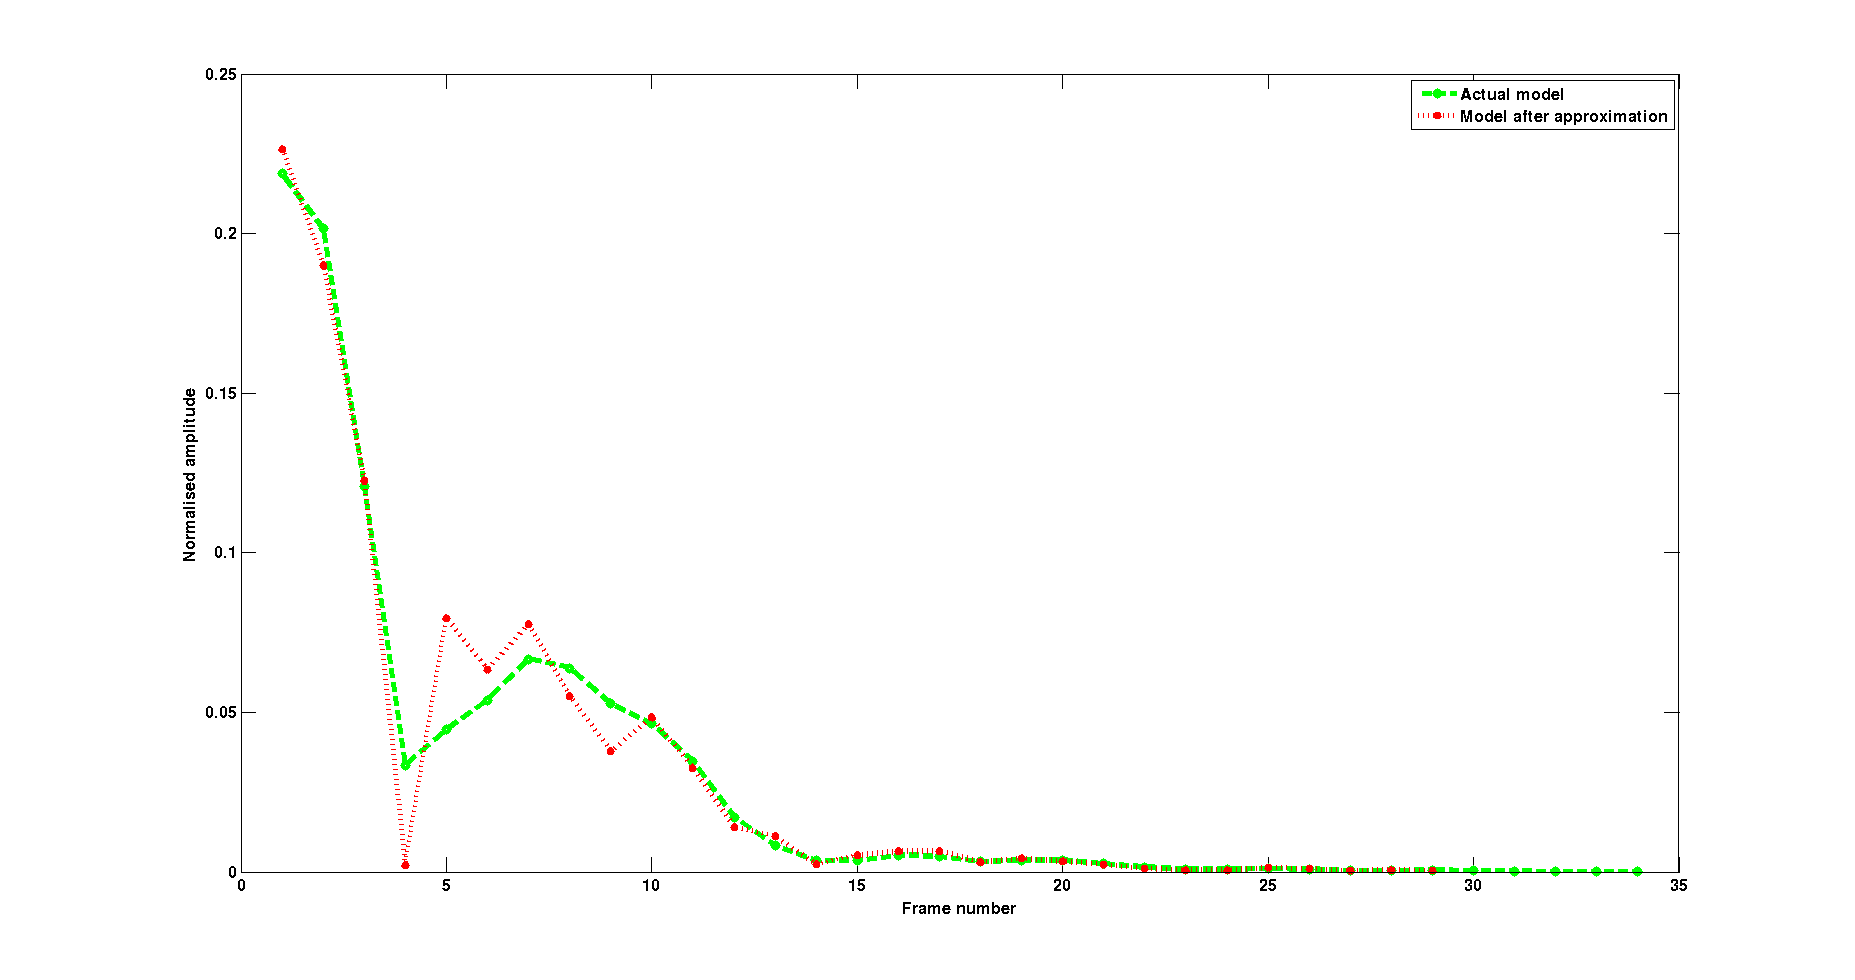
\includegraphics[width=9cm, height=6cm]{narrow_band_RIR_model}
\caption{Comparison of estimate of H with the actual H for k fixed at 50}
\label{fig:compare_true_expected}
\end{figure}

We compare the estimated $\mat{H}$ obtained using the reference approaches (N-CTF and N-CTF+NMF) to the
$\tilde{\mat{H}}$ for a RIR of $T_{60}$ approximately $700$~ms. These narrow band estimate of RIR obtained by reference methods with the actual value is plotted in Fig.~\ref{fig:compare_RIR_NMF}. It can be seen that the estimated RIR matches the expected RIR more closely during the later part of the RIR.  In the early part of the RIRs, the estimates are more erroneous, when compared to
the later parts. This is one of the main motivations for the proposed approach,
where we intend to use appropriate regularizer on $\mat{H}$ in the NMF approach
so that the estimated $\mat{H}$ is improved. Such an improved estimate for RIR,
will also lead to a better estimate of the speech signal leading to improved
speech enhancement and automatic speech recognition measures.
\begin{figure}
\centering
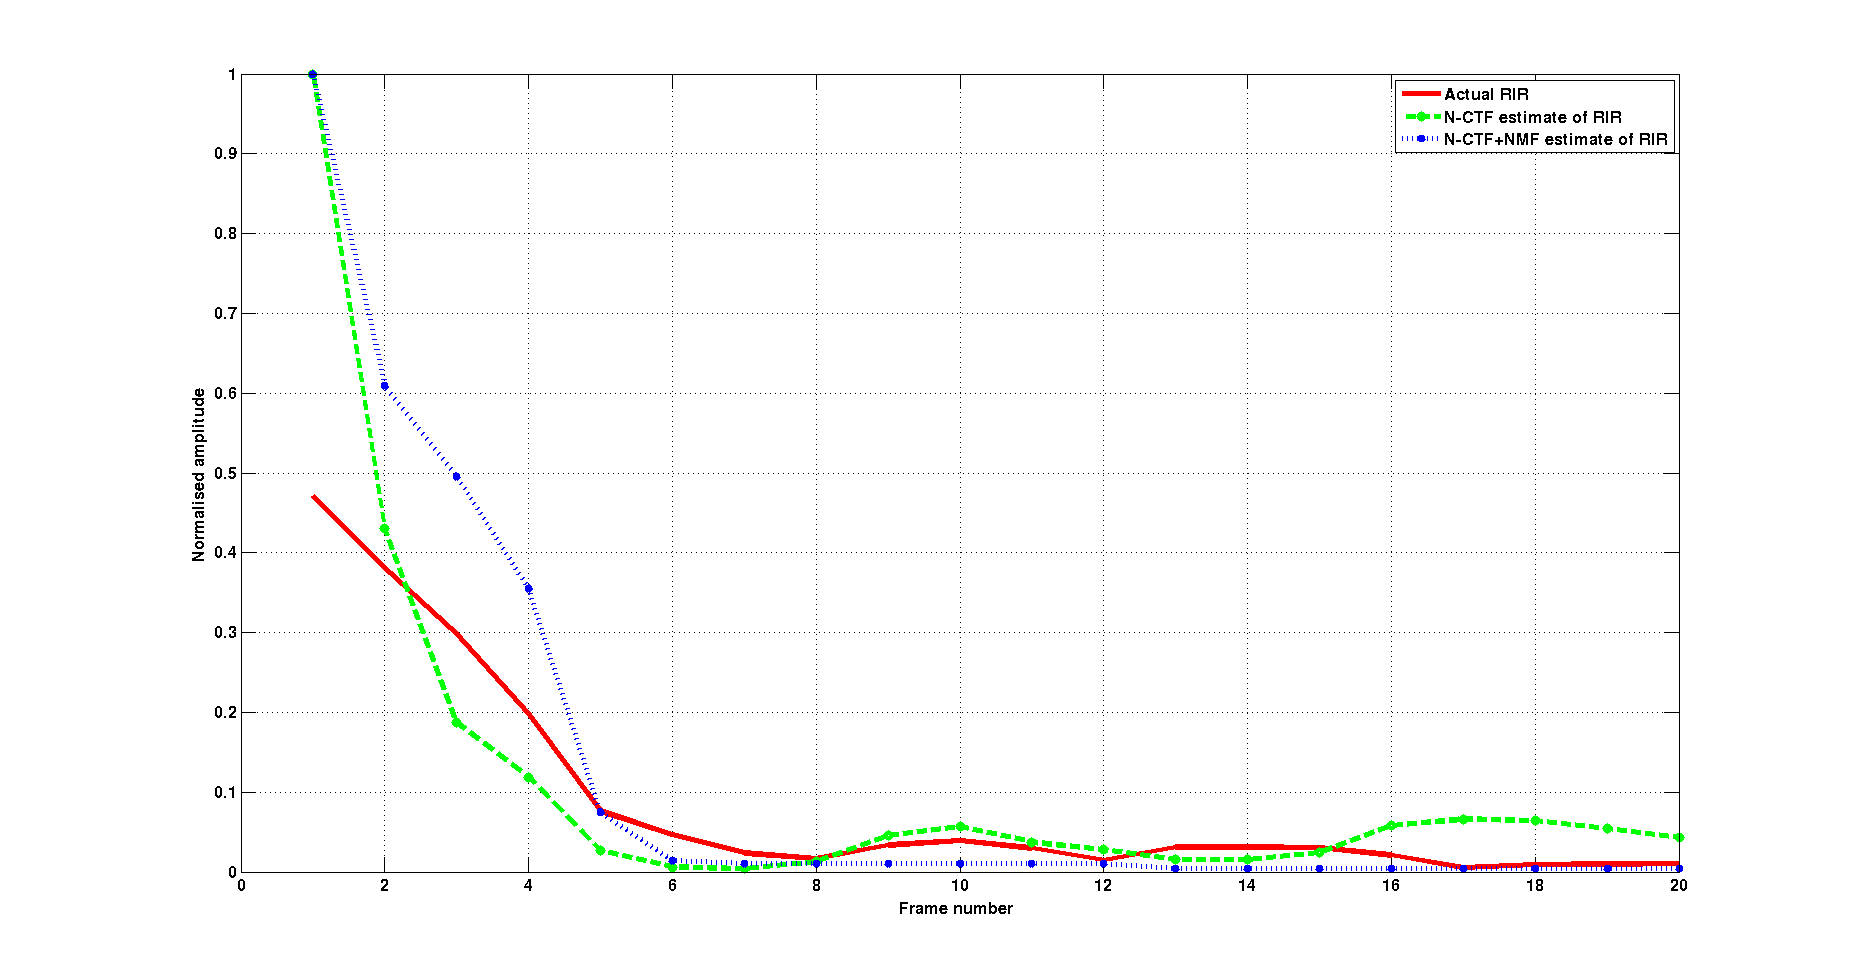
\includegraphics[width=9cm, height=6cm]{narrow_band_RIR}
\caption{Comparison of estimate of H with the actual H for k fixed at 50}
\label{fig:compare_RIR_NMF}
\end{figure}

% justification of early/late reflection effects in the reverberated speech signal
% XXX mention about regularizer used in multi-channel case
We propose three possible regularizations to the $\mat{H}$ for obtaining better
estimates of $\mat{H}$. We discuss the three choices and the corresponding cost
function.
\subsection{Sparsity of RIR}
\label{ssec:sparse_RIR}
Characterising RIRs of a reverberant room is challenging, as the RIRs depends on the room characteristics and distance between the source and the microphone acquiring the signal. However, the time-domain model by Pollack is a reasonable
characterisation based on the $T_{60}$ of a room model. Similarly, the
frequency-domain characterisation by Schroder is also a good model that has been
used extensively \cite{naylor2010speech}. It does not provide a characterisation of the
frequency-response but provides a characterisation of the possible distribution
of power with respect to frequency. In time-domain the RIR is exponentially
decaying with the decay factor dependent on the $T_{60}$. Correspondingly the
frequency domain representation of the RIR also has larger magnitude values
during the early part of the reverberation and the magnitude spectrum dies down
to smaller values during the late part. Most of the entries in H has a value very close to zero. Hence the simplest constraint is to
assume that the $\mat{H}$ has a sparse structure. This is different from
assuming sparsity on the speech signal. Assuming sparsity on $\mat{H}$ is
similar to assuming a sparse basis vector matrix in the standard NMF domain. We incorporate this into the basic NMD framework and have the modified
cost-function,
\begin{align}
  J(\mat{W}, \mat{X},\mat{H}) &= D_{KL}\left(\mat{Y}, \mat{X}\right),\\
  &= D_{LS}\left(\mat{Y}, \sum_{m} \mat{H}_m \stackrel{m\rightarrow}{\mat{S}}\right)
  + \lambda \parallel \mat{H} \parallel_1 \\
  \text{s.t.} & \mat{H}_m \ge 0, \mat{S} \ge 0.
  \label{eqn:NMFD_NMFcost_prop1}
\end{align}
$\lambda$ decides the weight given to sparsity of H. In the work, $\lambda = 1$. This method is referred to as N-CTF+Sparse H.
\subsection{Sub-band gains constrained RIR}
\label{ssec:gain_RIR}
Depending on the $T_{60}$ of the room and the distance between the source and
microphone the sub-band gain in the RIRs can be modelled as a function of the
frequency $Gain[k]$. Such models can be obtained by fitting
polynomial functions on existing recorded RIRs and their STFTs. This can be
included in the NMD framework as opposed to constraining the sub-band sums of
$\mat{H}$ to be unity. The corresponding cost function is,   
\begin{align}
  J(\mat{S},\mat{H}) &= D_{KL}(\mat{Y}, \mat{X}),\\
  &= D_{KL}\left(\mat{Y}, \sum_{m} \mat{H}_m
  \stackrel{m\rightarrow}{\mat{S}}\right) \\
  \text{s.t.} \sum_m H[k,m] = Gain[k],\ & k\in\{0,1,...,K-1\}\\
  \mat{H}_m \ge 0, \mat{S} \ge 0
  \label{eqn:NMFD_NMFcost_prop2}
\end{align}
where the $Gain[k]$ is to be obtained from existing RIRs or RIR models. This model is referred to as N-CTF+Gain H. 

\subsection{Inclusion of early part of RIR}\label{ssec:Hear_RIR}
RIR can be broadly divided into two regions - early reverberation and reverberation tale (late reverberation). The early part accounts for the reflections which come up to 50ms after the direct path. The reflections which come after 50 ms forms the reverberation tale. A sample RIR is shown in the fig. \ref{fig:RIR_plot}. The early part modifies the spectrum within a phone region, whereas the late reverberation results in changing the spectral characteristics of the present phone by the preceding phone. It is shown in the literature that late reverberation causes degradation of speech and need to be removed. However, retaining the early part improves speech intelligibility and ASR performance \cite{naylor2010speech}\cite{delcroix2014linear}. Once the clean 
speech spectrum ($S$) is estimated, the early part of RIR ($H_{ear}$) is attached to it using the following equation to obtain an improved dereverberated spectrum ($S_{new}$). 
\begin{figure}
\centering
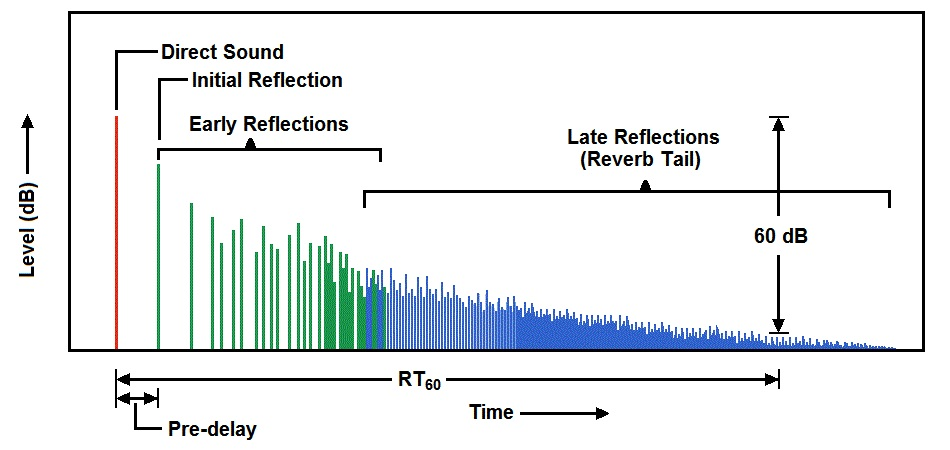
\includegraphics[width=8cm, height=6cm]{reverberation2}
\caption{Time domain representation of a typical RIR~\cite{rir_plot}}
\label{fig:RIR_plot}

\end{figure}
\begin{equation}
S_{new}(n,k) = S(n,k)*H_{early}(n,k), k\in\{0,1,...,K\}
\end{equation}
This method is referred to as N-CTF+$H_{ear}$. The algorithm using both N-CTF+$H_{ear}$ and N-CTF+Gain H is refereed to as N-CTF+$H_{ear}$+Gain H.
%\section{Formatting your paper}
%\label{sec:format}
%
%All printed material, including text, illustrations, and charts, must be kept
%within a print area of 7 inches (178 mm) wide by 9 inches (229 mm) high. Do
%not write or print anything outside the print area. The top margin must be 1
%inch (25 mm), except for the title page, and the left margin must be 0.75 inch
%(19 mm).  All {\it text} must be in a two-column format. Columns are to be 3.39
%inches (86 mm) wide, with a 0.24 inch (6 mm) space between them. Text must be
%fully justified.

\section{Results}
The performance of the algorithms discussed in section~\ref{prop_method} are evaluated for both speech enhancement and automatic speech recognition tasks (ASR).
\subsection{Database}
Two databases (TIMIT and TIDIGITS) have been used for the experiments. TIMIT contains two sets of data (train and test). Train set contains 10 sentences spoken by 377 different speakers and test set contains 10 sentences spoken by 168 distinct speakers. There are no common speakers in test and train sets. Out of the 10 sentences, 2 Sentences is common across all speakers. The performance in speech enhancement task is compared using a subset of TIMIT database. A set of 16 different sentences spoken by 16 distinct speakers is used. TIDIGITS contains 112 distinct adult speakers (55 male and 57 female) in train set and 113 different adult speakers (56 male and 57 female) in the test set. Each speaker has 77 utterances.  The database contains 11 distinct words (zero to nine and oh). The ASR performance is evaluated using adult data set of TIDIGITS. 

The word error rate (WER) of TIMIT database is relatively high ($\approx28\%$) for clean speech. Since the best achievable WER is itself high, a reliable WER improvement of various dereverberation algorithms cannot be analyzed using the database. The relative improvement in objective measures for the reference method using TIMIT database is available in \cite{mohammadiha2016speech}. To verify the implementation of reference method, TIMIT database is used for speech enhancement task. TIDIGITS is a limited vocabulary database with very low WER ($\approx1.5\%$). So TIDIGITS is used for comparing the performance of various algorithms for ASR task.   
\subsection{Evaluation measures}
The improvement in speech enhancement task is compared using improvement in three objective measures - perceptual evaluation of speech quality (PESQ), cepstral distance (CD) and speech-to-reverberation modulation energy ratio  (SRMR) \cite{falk2010non} \cite{reverb2014}. Dereverberated speech increases PESQ and SRMR score while CD tend to decrease as compared to reverberated speech. The effectiveness of the dereverberation algorithms is compared using the relative change in the objective measures of dereverberated speech ($\Delta PESQ$, $\Delta CD$ and $\Delta SRMR$) as compared with the reverberated speech.

Speech recognition performance is compared using the improvement in word error rate (WER) as compared to the reverberated speech. Speech recognition is performed using Kaldi toolkit trained on TIDIGITS. The speech recognition system has three sources of error - insertion, deletion, and substitution. For this task, the WER is defined as the ratio of the total number of misclassified phones to the total number of phones in the test set. Mathematically,
\begin{equation}
WER = \dfrac{INS + DEL + SUB}{Total\ number\ of\ phones\ in\ test\ set}*100\%
\end{equation}
where $INS$, $DEL$, $SUB$ represents the total number of insertion, deletion and substitution errors while decoding in the test set respectively. 
\subsection{Reference methods}
Two dereverberation algorithms NCTF and NCTF with speech model \cite{mohammadiha2016speech} are used as reference methods for comparison. In the reference paper, the objective measures PESQ, and CD were used for verifying the performance of the algorithm. The algorithm was tested on reverberated data generated using $16$ different TIMIT sentences which are spoken by $16$ distinct speakers. Reverberation is simulated using a measured RIR having a $T_{60}$ of around $680$~ms and DRR of $0$~dB was used. The NCTF model showed an improvement of about $0.3$ in PESQ score and $0.5$ in CD as compared to reverberated speech. The NCTF with speech model showed an improvement of $0.4$ in PESQ score and $0.4$ CD as compared to reverberated speech. The implementation of this method is verified by trying to reproduce the results in \cite{mohammadiha2016speech}. Although the exact RIR and set of sentences used in the experiments are unknown, we chose an RIR which has a $T_{60}$ and DRR of roughly $700$~ms and $0$~dB. Also, a subset of $16$ sentences spoken by different speakers from TIMIT database was used for performance evaluation. A PESQ score improvement of $0.46$ and CD improvement of $0.08$ is obtained for N-CTF method. Also, for N-CTF with speech model, a PESQ and CD improvement of $0.65$ and $0.1$ were obtained. The improvement obtained in PESQ score is comparable with the score obtained in \cite{mohammadiha2016speech}. However, improvements in CD was not comparable with the reference paper. The difference in obtained objective measure scores with the reference paper could be because of the different RIR and set of sentences used in the experiments. The implemented of algorithms are tested for other RIRs. Table \ref{tab:comparison_enhancement} shows the objective measure improvement for a different set of RIRs. Both PESQ and CD improves significantly improved for the reference methods. 
\subsection{Experiment setup}
The magnitude spectrogram is obtained using a $64$~ms window with a hop size of $16$~ms. The square root of Hanning window is used in analysis and synthesis side. The magnitude spectrogram of RIR (H) is represented using 20 frames. Out of which the first $2$ frames is related to the combination of direct path and early reverberation. H for each narrowband is initialized as a linearly decreasing function. S is initialized as the spectrogram of reverberated speech. For models with speech model, initial values for the basis and the activations are obtained by performing NMF decomposition on the spectrogram of reverberated speech. Since the algorithms converge fast, 20 iterations are performed for each algorithm to obtain the estimates of S and H.

Measured RIRs available from REVERB challenge \cite{reverb2014} is used for the evaluation. The RIRs are measured using an $8$ channel circular array of diameter $10$~cm. The RIRs of three rooms (small, medium and large) with $T_{60}$ of $250$~ms, $500$~ms and $700$~ms are available. The recordings are done for a microphone array placed $0.5$~m and $2$~m away from the source. 
The particular RIRs used for the experiment were measured in a room having a $T_{60}$ of $700$~ms with the microphone array placed $2$~m distant from the source. A similar trend in the dereverberation performance was observed for other RIRs. The dereverberation algorithms are performed by treating the 8 channel reverberated data as 8 independent recordings. 
\subsection{Speech enhancement for the proposed methods}
The performance of proposed dereverberation algorithms is compared using different objective measures. Since the microphones are placed very close to each other, the relative improvement in objective measures obtained across 8 channels is very close to each other. The net enhancement in the performance of different algorithms is obtained as an average of improvement in the objective measures for 16 sentences across 8 channels. The average objective measure improvement for various algorithms is shown in the Table \ref{tab:comparison_enhancement}.

From Table \ref{tab:comparison_enhancement}, it is observed that the baseline dereverberation algorithms N-CTF and N-CTF+NMF are able to enhance the reverberated speech.  Inducing sparsity (N-CTF+Sparse H) and frequency envelope on H (N-CTF+Gain H) does not improve the performance. 
The reason for the sparse H showing no improvement could be that narrow band H roughly has the exponentially decaying structure which we hope to achieve. 
The multiplicative update for the cost function in \eqref{eqn:NMFD_NMFcost_prop2} is obtained such that it minimizes the error in each narrowband independently. 
So the in effect cost function remains the same even after putting frequency envelope in H. 
All the objective measures show improvement for N-CNMF+$H_{early}$. However,  for N-CNMF+NMF+$H_{early}$, SRMR shows a significant improvement while other measures remain unchanged. The possible explanation can be that the algorithm reduces reverberation but also  adds distortion to the dereverberated speech. 
\begin{table}[th]
        \caption{\label{tab:comparison_enhancement} {\it The improvement in objective measures
        obtained using the proposed regularization to the RIR are compared with
      existing NMF based approaches.}}
        \vspace{2mm}
        \centerline{
          \begin{tabular}{|l|c|c|c|} \hline
            Methods & $\Delta PESQ$ & $\Delta CD$ & $\Delta SRMR$ \\ \hline \hline         
            N-CTF & $0.286$ & $0.671$& $1.200$\\
            N-CTF + $\mat{H_{early}}$ & $0.356$ & $0.722$& $1.611$\\
            N-CTF + Gain $\mat{H}$ & $0.278$ & $0.659$& $1.008$\\
            N-CTF + $\mat{H_{early}}$ + Gain $\mat{H}$ & $0.364$ & $0.718$& $1.557$\\
            N-CTF + Sparse $\mat{H}$ & $0.286$& $0.671$& $1.200$\\
            N-CTF + NMF speech & $0.570$& $0.909$& $1.236$\\
            N-CTF + NMF speech + $\mat{H_{early}}$ & $0.525$& $0.914$& $1.883$\\            
            \hline
          \end{tabular}
       }
\end{table}
\subsection{ASR improvement for the proposed methods}

The speech recognition system using Kaldi toolkit was trained using a Gaussian mixture model (GMM) - hidden Markov model (HMM) system. The system was trained using training data set of TIDIGITS. It contains 56 male and 58 female speakers speaking 77 utterances each. The GMM is an 8 Gaussian mixture. The HMM is a monophone with 1000 tied states. The ASR results obtained for an RIR with $T_{60}$ of $700$~ms and $2$~m away from the source is shown in Table \ref{tab:comparison_asr}.

The N-CTF model shows significant improvement in WER.  
N-CTF+Sparse H and N-CTF+Gain H methods show no improved the performance.
N-CTF+$H_{early}$ shows marginal improvement.
Methods including speech model (N-CTF+NMF and N-CTF+NMF+$H_{early}$) also show marginal improvement over N-CTF even though the objective measures shown significant improvement. The reason could be that dereverberation using speech model induced artifacts which do not affect the enhancement but affected the ASR performance. 
This can be observed in the estimate of H which shows distortions whereas for the N-CTF, the H estimate is smooth. N-CTF+NMF+$H_{early}$ has no significant improvement in ASR results as compared to N-CTF+NMF. 
\begin{table}[th]
        \caption{\label{tab:comparison_asr} {\it The improvement
        obtained for ASR task using the proposed regularization to the RIR are compared with
      existing NMF based approaches.}}
        \vspace{2mm}
        \centerline{
          \begin{tabular}{|l|c|c|} \hline
            Methods & $WER(\%)$ & $\Delta WER (\%)$  \\ \hline \hline  
            Clean speech & $1.76$ & $-$\\
            Reverberated speech &$29.03$ & $-$\\      
            N-CTF & $19.97$ & $9.06$\\
            N-CTF + $\mat{H_{early}}$ & $19.26$ & $9.77$\\
            N-CTF + Gain $\mat{H}$ & $20.06$ & $8.97$\\
            N-CTF + $\mat{H_{early}}$ + Gain $\mat{H}$ & $19.61$ & $9.42$\\
            N-CTF + Sparse $\mat{H}$ & $19.50$& $9.53$\\
            N-CTF + NMF speech & $19.24$& $9.79$\\
            N-CTF + NMF speech + $\mat{H_{early}}$ & $19.21$& $9.82$\\            
            \hline
          \end{tabular}
       }
\end{table}
\subsection{ASR improvement on beamformed output}
This section discusses the ASR performance a 2 stage dereverberation system. In the first stage, beamforming is performed using BeamformIt toolkit \cite{anguera2007acoustic} to obtain an enhanced single channel data obtained from 8 channel data. The second stage is a single channel dereverberation methods using the proposed methods. The second stage reduces the residual reverberation present after beamforming. The reverberation conditions and training set are same as in earlier experiments, but testing is done in a reduced set of 6 speakers (3 males and 3 females).

Table \ref{tab:comparison_asr_red1} shows the ASR performance of dereverberation using beamforming and proposed methods. The reference method N-CTF shows improvement in WER as compared with the beamformed output. This shows that the algorithm is able to suppress the residual reverberation present in the channel after beamforming. Other proposed algorithms failed to improve the WER any further. Table \ref{tab:comparison_asr_red2} compares the performance of proposed methods for the beamformed output in the presence of reverberation and noise. The algorithms perform poorly. The reason could be that the algorithm is designed to model reverberation alone. So in the presence of residual noise after beamforming, the algorithm fails to produce a good estimate of clean speech.  
\begin{table}[th]
        \caption{\label{tab:comparison_asr_red1} {\it The improvement in reverb speech ASR
        obtained using the beamforing followed by proposed methods.}}
        \vspace{2mm}
        \centerline{
          \begin{tabular}{|l|c|c|} \hline
            Methods & $WER(\%)$ & $\Delta WER (\%)$  \\ \hline \hline  
            Clean speech & $1.32$ & $-$\\
            Reverberated speech &$27.15$ & $-$\\  
            Beamforming & $22.2$ &$4.96$\\    
            N-CTF & $16.34$ & $10.82$\\
            N-CTF + $\mat{H_{early}}$ & $16.47$ & $10.69$\\
            N-CTF + NMF speech & $16.6$& $10.56$\\
            N-CTF + NMF speech + $\mat{H_{early}}$ & $17.33$& $9.83$\\            
            \hline
          \end{tabular}
       }
\end{table}
\begin{table}[th]
        \caption{\label{tab:comparison_asr_red2} {\it The improvement in reverb+noise(10dB) speech ASR
        obtained using the beamfoming followed by proposed methods.}}
        \vspace{2mm}
        \centerline{
          \begin{tabular}{|l|c|c|} \hline
            Methods & $WER(\%)$ & $\Delta WER (\%)$  \\ \hline \hline  
            Clean speech & $1.32$ & $-$\\
            Reverberated speech &$56.19$ & $-$\\  
            Beamforming & $41.63$ &$17.88$\\    
            N-CTF & $77.93$ & $-18.42$\\
            N-CTF + $\mat{H_{early}}$ & $77.87$ & $-18.36$\\
            N-CTF + NMF speech & $73.06$& $-13.55$\\
            N-CTF + NMF speech + $\mat{H_{early}}$ & $53.69$& $5.82$\\            
            \hline
          \end{tabular}
       }
\end{table}
\section{Conclusions and future work}
 The speech enhancement and ASR performance of speech dereverberation algorithms for various constraints on RIR are studied. 
The addition of sparsity and frequency envelope of RIR does not change the speech enhancement performance of the algorithm as compared with the baseline N-CTF model. But the inclusion of early part of RIR ($H_{early}$) with the estimate of clean speech improved the objective measures. The objective measures for reference method with speech model (N-CTF+NMF) also showed  improvement when $H_{early}$ was included in the model. 

The dereverberation using C-NMF reduced significantly the ASR performance. The inclusion of sparsity and frequency envelope did not change the WER. $N-CTF+H_{early}$ method shows a marginal improvement in ASR performance.  The inclusion of speech model ($N-CTF+NMF$) also did not show significant improvement in ASR performance. However, the algorithms were able to residual reverberation present in a beamformed output, but the algorithm fails to improve the performance in the presence of background noise. 
 
The dereverberation algorithms are not able to completely remove the effects of reverberation. A better model for reverberation and speech could improve the performance of dereverberation algorithm. Replacing NMF model for the clean speech by a convolutive NMF model could be one such approach. The use of multichannel data helps in dereverberation \cite{naylor2010speech}. The proposed methods can be modified to handle multichannel data. Also, other multichannel dereverberation algorithms like beamforming have to be studied. The effects of noise in distance speech recording are unavoidable. The performance of dereverberation algorithms is affected by the presence of noise. The proposed methods perform poorly in the presence of noise as discussed in section. So there is a need for modifying the proposed models to include the effects of noise. Other methods which perform dereverberation and denoising together should also need to be studied.  

\fi
\chapter{Separability Assumption on RIR Spectrogram}
\label{chapter:interspeech2018}

\section{NMF degradation models}
\begin{itemize}
\item Derivation
\begin{itemize}
\item NMF model for reverberation
\item Extended model for reverberation and noise
\end{itemize}
\end{itemize}
\section{Analysis of model}
\begin{itemize}
\item Effect of reverberation on clean speech bases and activation
\end{itemize}
\section{Enhancement algorithm}
\begin{itemize}
\item cost function
\item multiplicative update rule
\item normalization used 
\end{itemize}
\section{Experimental results}
\begin{itemize}
\item enhancement results
\item RIR estimates
\end{itemize}
\section{Discussion}
\begin{itemize}
\item comparison of results
\item limitations
\end{itemize}

\iffalse
In many real-world applications such as smart homes, robots, conference meetings, and voice-controlled personal assistants speech recordings are done using microphones placed few meters away from the source. Such distant speech recordings (DSRs) are severely affected by reverberation and background noise~\cite{naylor2010speech}. This degrades speech intelligibility and performance of automatic speech recognition performance (ASR) systems. Speech enhancement helps in improving speech intelligibility and can be used as a pre-processing step for improving ASR~\cite{kinoshita2016summary}. The effects of reverberation depend on the properties of speech and room impulse response (RIR). Speech dereverberation can be done using single- or multi-channel data depending on the application of interest. In this work, we address single-channel dereverberation in the DSR scenario.

Dereverberation methods proposed in the literature include reverberation cancellation methods, blind deconvolution based methods, and reverberation suppression methods such as spectral subtraction, linear prediction (LP) and non-negative matrix factorization (NMF) based methods~\cite{naylor2010speech}. The earliest work on NMF based dereverberation~\cite{kameoka2009robust} uses a convolutive NMF (referred as C-NMF) model for the reverb spectrogram. Since then many modifications to this have been proposed both in single-channel~\cite{Kumar2011,mohammadiha2016speech,Mohammadiha2015,baby2015coupled,Kallasjoki2014} and multi-channel scenario~\cite{Mirsamadi2014}. In~\cite{Kallasjoki2014}  the C-NMF model is shown as a special case of NMF decomposition. The C-NMF model for speech dereverberation was improved by additionally incorporating a NMF model for clean speech~\cite{mohammadiha2016speech, Mohammadiha2015}. Various supervised approaches to handle reverberation in noisy environments have also been proposed~\cite{baby2015coupled, baby2016phd, baby2017joint}.  
Different regularization on RIRs in single-channel~\cite{baby2017joint,mohanan2017speech} and multi-channel~\cite{Yu2014} scenario have been proposed leading to better speech enhancement. In contrast to these methods that use C-NMF for dereverberation, we propose a NMF model for reverberation. The model uses magnitude spectrogram of the reverb speech and learned clean speech bases to estimate the enhanced speech. Such an approach will allow us to incorporate meaningful constraints in the frequency- and time-domain. This leads to a better speech enhancement, as it has direct control over the estimates of clean speech activations and better RIR estimates. Another advantage of such a model is that it can be easily extended to handle additive noise making it suitable for a noisy reverberant scenario. 
%The NMF methods are evaluated using speech enhancement measures such as CD and SRMR~\cite{hu2008evaluation, falk2010non}.
%Dereverberation methods proposed in the literature include reverberation cancellation methods, blind deconvolution based methods and reverberation suppression methods such as spectral subtraction, linear prediction (LP) based methods~\cite{naylor2010speech}. We propose a reverberation suppression method based on non-negative matrix factorization (NMF). The model uses magnitude spectrogram of the reverb speech and clean speech bases to estimate the enhanced speech.
%The earliest work on NMF based dereverberation~\cite{kameoka2009robust} uses a convolutive NMF (referred as C-NMF) model for the reverb spectrogram. Since then many  modifications to this have been proposed both in single-channel~\cite{Kumar2011,mohammadiha2016speech,Mohammadiha2015,baby2015coupled,Kallasjoki2014} and multi-channel scenario~\cite{Mirsamadi2014}. The original C-NMF model for speech dereverberation was improved by incorporating NMF models for the speech signals~\cite{mohammadiha2016speech, Mohammadiha2015}. Various supervised approaches to handle reverberation and noise have been proposed to handle reverberation in noisy environments~\cite{baby2015coupled, baby2016phd, baby2017joint}. In~\cite{Kallasjoki2014}  the C-NMF model is viewed as a NMF decomposition.
%Different regularization on RIRs in single-channel~\cite{baby2017joint,mohanan2017speech} and multi-channel~\cite{Yu2014} scenario have been proposed leading to better speech enhancement. In contrast to these methods that use C-NMF for dereverberation, we propose a NMF model for reverberation. Such an approach will allow us to incorporate meaningful constraints in the frequency- and time-domain. This leads to a better speech enhancement, as it has direct control over the estimates of clean speech activations and better RIR estimates. Another advantage of such a model is that it can be easily extended to handle additive noise making it suitable for noisy reverberant scenario. The NMF methods are evaluated using speech enhancement measures such as CD and SRMR~\cite{hu2008evaluation, falk2010non}.


\section{NMF based dereverberation}

Reverberated speech $y(t)$ recorded at a microphone is expressed as the convolution of clean speech $s(t)$ and the RIR $h(t)$~\cite{naylor2010speech}. %\textbf{[($y(t)=s(t)*h(t)$)]}~\cite{naylor2010speech}.
%\begin{equation}
%y(t) = h(t) * s(t)
%\label{eq:deg1}
%\end{equation}
%In the magnitude spectrogram domain, the degradation is approximated as the sum of spectrograms due to reverberation and noise. 
%\subsection{C-NMF model for reverberation}
In the absence of noise, speech degradation due to reverberation can be modeled in the magnitude spectrogram domain by utilizing the modulation transfer function (MTF) model for reverberation~\cite{kameoka2009robust}. According to the MTF  model, the magnitude envelope for each subband of reverberant speech magnitude spectrogram ($\mathbf{Y}$) can be approximated as the convolution of the corresponding subband magnitude envelopes of the RIR ($\mathbf{H}$) and the clean speech ($\mathbf{S}$) spectrograms~\cite{Kumar2011}. Accordingly, 
\begin{equation}
Y(k,n) \approx H(k,n)*_n S(k,n)=\sum_{l=0}^{L_h-1}H(k,l)S(k,n-l)\text{,}
\label{eq:deg2}
\end{equation}
where, $Y(k,n)$, $H(k,n)$ and $S(k,n)$ represent the $(n,k)$-th element of $\mathbf{Y}$, $\mathbf{H}$ and $\mathbf{S}$, respectively, $L_h$ represents the number of frames used to represent the RIR spectrogram $\mathbf{H}$ and $*_n$ represents convolution across frame index. The model in~(\ref{eq:deg2}) can be viewed as a convolutive NMF (C-NMF) decomposition where $\mathbf{H}$ and $\mathbf{S}$ can be obtained using multiplicative updates~\cite{kameoka2009robust}.

%The model in (\ref{eq:deg2}) was improved in \cite{mohammadiha2016speech,Mohammadiha2015} to use a NMF model for speech spectrogram. 
The speech enhancement results using the model in (\ref{eq:deg2}) were improved by incorporating a NMF model for the magnitude spectrogram of clean speech~\cite{mohammadiha2016speech,Mohammadiha2015}.
They exploit the low-rank nature of clean speech spectrogram by having a NMF decomposition on clean speech spectrogram $S(k,n)$ as,
\begin{equation}
S(k,n)\approx\sum_{r=1}^R W_{s}(k,r)X_{s}(r,n)\text{,}
\label{eq:nmf1}
\end{equation}
where $W_{s}(k,r)$, $X_s(r,n)$ are elements of the bases, activations and $R$ is the rank of the decomposition. Using (\ref{eq:nmf1}) in (\ref{eq:deg2}),
\begin{equation}
Y(k,n) \approx \sum_{l=0}^{L_h-1}H(k,l)\bigg(\sum_{r=1}^R W_{s}(k,r)X_{s}(r,n-l)\bigg)\text{.}
\label{eq:deg4}
\end{equation}
From (\ref{eq:deg4}), enhanced speech is obtained by solving for $H(k,l)$, $W_{s}(k,r)$ and $X_{s}(r,n)$ iteratively. This method will be referred to as C-NMF+NMF. In \cite{mohammadiha2016speech,Mohammadiha2015}, several approaches to obtain bases are experimented with. In online (unsupervised) methods, the bases are learned from the reverberant speech. In offline (supervised) methods, the bases are learned from clean speech utterances. The proposed approach uses supervised bases, so we use the offline method as a baseline for comparison. The joint speech dereverberation and denoising methods using C-NMF model~\cite{baby2015coupled, baby2016phd, baby2017joint} are not compared as they use exemplar bases, which require a large number of bases when compared to learned bases to represent clean speech.   

%\subsection{Proposed non-convolutive NMF model for reverberation}
\subsection{Proposed non-convolutive NMF model}
\label{sec:PropNMF}
%In the proposed method, an alternate approach to perform dereverberation using NMF is discussed. A two stage algorithm is proposed to perform dereverberation. In the first stage, a supervised NMF decomposition is performed on reverb spectrogram. This stage assumes that the clean speech basis can model reverb spectogram. The basis vectors are learned from clean utterances. In the second stage, clean speech activations are obtain from the reverb activations using a CNMF decomposition. The two stage approach is made possible by having additional constrain on RIR spectrogram that it varies similarly in different subbands ($H(f,n)=H(n)\forall f$). Mathematically, the two stages can be written as,
We propose a method to perform dereverberation by representing the reverb spectrogram using a non-convolutive NMF as, $\mathbf{\tilde{Y}}=\mathbf{W}_R\mathbf{X}_R$, where $\mathbf{W}_R$ and $\mathbf{X}_R$ represent the bases and activation of this decomposition. Such a model is made possible by having a separability assumption on the RIR spectrogram $H(n,k)=H_1(k)H_2(n)$. 
This approximation is based on the following observations. 
Firstly, the RIR magnitude spectrum across frequencies for different frames is similar and has a decaying structure across time as is observed in literature~\cite{wen2008blind}. Secondly, the subband magnitudes of the RIR for different frequencies decay with time. The rate of decay with time for different subband is assumed to be same. Combining these observations, a simplifying model will be to write $H(n,k)$ as having a frequency envelope $H_1(k)$ with a gain $H_2(n)$ for different frames.
%The algorithm can be improved by incorporating the frequency dependence of $T_{60}$~\cite{jeub2010we}.
%Firstly, the RIR spectrogram for different frames approximately follows the same frequency structure. It can be observed that some frequency bands of RIR spectrogram have higher magnitude while others have lower values. The presence of frequency envelope for RIR spectrogram is also reported in the literature~\cite{wen2008blind}.  Secondly, the magnitudes of RIR spectrograms for all frequency bands decay down with time.  Combining these observations, a simplifying model will be to write $H(n,k)$ as having a frequency envelope $H_1(k)$ with a gain $H_2(n)$ for different frames. The frequency dependence of $T_{60}$~\cite{jeub2010we} is ignored in this assumption.}
With this, we have
%This model is based on MTF model for reverberation. With a separability assumption on RIR spectrogram ($H(n,k)=H_1(k)H_2(n)$), the MTF model is replaced with a NMF model. $\mathbf{W}_R$ and $\mathbf{X}_R$ represents the bases and activation of this decomposition. The reverb spectrogram ($\tilde{\mathbf{Y}}$) can be is written as,

\begin{align}
\tilde{Y}&(k,n) = \sum_{l=0}^{L_h-1} H_1(k)H_2(l) \sum_{r=1}^R W_{s}(k,r)X_{s}(r,n-l)\nonumber\\
& = \sum_{r=1}^R \underbrace{W_s(k,r)H_1(k)}_{W_R(k,r)} \underbrace{\sum_{l=0}^{L_h-1}H_2(n)X_s(r,n-l)}_{X_R(r,n)}
\label{eq:reverbNMF}
\end{align}
where, $\tilde{Y}(i,j)$, $W_R(i,j)$, and $X_R(i,j)$ are the $(i,j)$-th element of $\tilde{\mathbf{Y}}$, $\mathbf{W}_R$ and $\mathbf{X}_R$, respectively. Equation~(\ref{eq:reverbNMF}) is a NMF decomposition with rank $R$ of the reverb spectrogram. The set of bases and activations obtained from this decomposition is related to clean speech bases and activations. The reverb bases ($W_R(k,r)=W_s(k,r)H_1(k)$) are the clean speech bases $W_s(k,r)$ modified by the frequency envelope of the RIR spectrogram $H_1(k)$.
%All the clean speech bases are modified by a frequency envelope RIR spectrogram ($H_1(k)$) to obtain the reverb bases ($W_R(k,r)=W_s(k,r)H_1(k)$). 
The reverb activations are obtained as the convolution of clean speech activations with the time-dependent envelope of the RIR ($X_R(r,n)=X_s(r,n)*_nH_2(n)$). Estimation of these parameters is done in two steps. In the first step, with the knowledge of learned speech bases, $H_1(k)$ and reverb activations are learned from the reverb spectrogram. Generalized Kullback-Leibler (KL) divergence is used as the distance measure in the first stage as this is related to speech~\cite{mohammadiha2016speech}. The NMF cost function ($C$) is given as, 
\begin{equation}
C = \sum_{n,k} \bigg[Y(k,n)\text{ln}\bigg(\dfrac{Y(k,n)}{\tilde{Y}(k,n)}\bigg) - Y(k,n) + \tilde{Y}(k,n)\bigg]
\label{eq:C}
\end{equation}
Multiplicative update rules are obtained for $H_1(k)$ and $X_R(r,n)$ using the cost function in (\ref{eq:C}). The updates obtained are,
\begin{align}
H_1(k)&\leftarrow H_1(k) \dfrac{\sum_{n,r} \dfrac{Y(k,n)}{\tilde{Y}(k,n)} W_s(k,r)X_R(r,n)}{\sum_{n,r} W_s(k,r)X_R(r,n)}\text{, and}\nonumber\\
X_R(r,n)&\leftarrow X_R(r,n) \dfrac{\sum_k \dfrac{Y(k,n)}{\tilde{Y}(k,n)}H_1(k)W_s(k,r)}{\sum_k H_1(k)W_s(k,r)}
\label{eq:updateProp}
\end{align} 
In the second stage, clean activations are learned from reverb activations. The second stage uses Euclidean distance as the distance measure to estimate clean activations from reverb activations, since the estimated parameters are no longer related to speech as in (\ref{eq:C}) and can be viewed as a general signal. The NMF cost function in this case is defined as,
\begin{equation}
C_1 = \sum_{r,n}( X_R(r,n) - H_2(n) *_n X_s(r,n))^2
\end{equation}
Simultaneous estimation of $X_s(r,n)$ and $H_2(n)$ from $X_R(r,n)$ leads to the trivial solution of $X_s(r,n)=X_R(r,n)$ and $H_2(n)$ being an impulse. To get a meaningful solution, $H_2(n)$ is initialized using prior knowledge of room and source-microphone distance in the RIR structure (Sec 4.1.3 in~\cite{kinoshita2016summary}).
% and $X_s(r,n)$ is updated. For example, Sec 4.1.3 in~\cite{kinoshita2016summary} discusses a model for time-dependent behavior of $H(n,k)$ using the knowledge of $T_{60}$. 
The update for $X_s(r,n)$ is given by,
\begin{equation}
X_s(r,p) \leftarrow X_s(r,p) \dfrac{\sum_n X_R(r,n)H_2(n-p)}{\sum_n\tilde{X}_R(r,n) H_2(n-p)}
\end{equation}
where, $\tilde{X}_R(r,n)$ is the estimated reverb activation ($\tilde{X}_R(r,n) = X_s(r,n)*_nH_2(n)$). The clean speech spectrogram can be estimated as $\hat{S}(k,n)=G(k,n)Y(k,n)$, where the gain function $G(k,n)$ is written as,
\begin{equation}
G(k,n)=\dfrac{\sum_rW_s(k,r)X_s(r,n)}{\tilde{Y}(n,k)}
\end{equation}
The proposed reverberation model using NMF will be referred to as R-NMF. 

We now justify the proposed model using an illustrative example, considering a reverberated TIMIT utterance obtained using a RIR with $T_{60}\approx700$~ms and source-microphone distance (d) of $0.5$~m. Using the first step, one can see that the reverb bases $W_R(k,r)$ are indeed the clean speech bases $W_s(k,r)$ acted upon by the frequency envelope of the RIR $H_1(k)$. The estimated frequency envelope of the RIR obtained using the proposed model is compared with the true frequency envelope $H^{\text{True}}_1(k)$ in Figure~\ref{fig:freqEnv_comp}. $H^{\text{True}}_1(k)$ is obtained as the average value of normalized frequency spectrum for the three frames of RIR spectrogram with maximum energy. From the figure, it is clear that for most frequencies, the estimated $H_1(k)$ is very close to $H^{\text{True}}_1(k)$. A similar behavior was observed for other RIRs. 

\begin{figure}[tbh!]
  \centering
  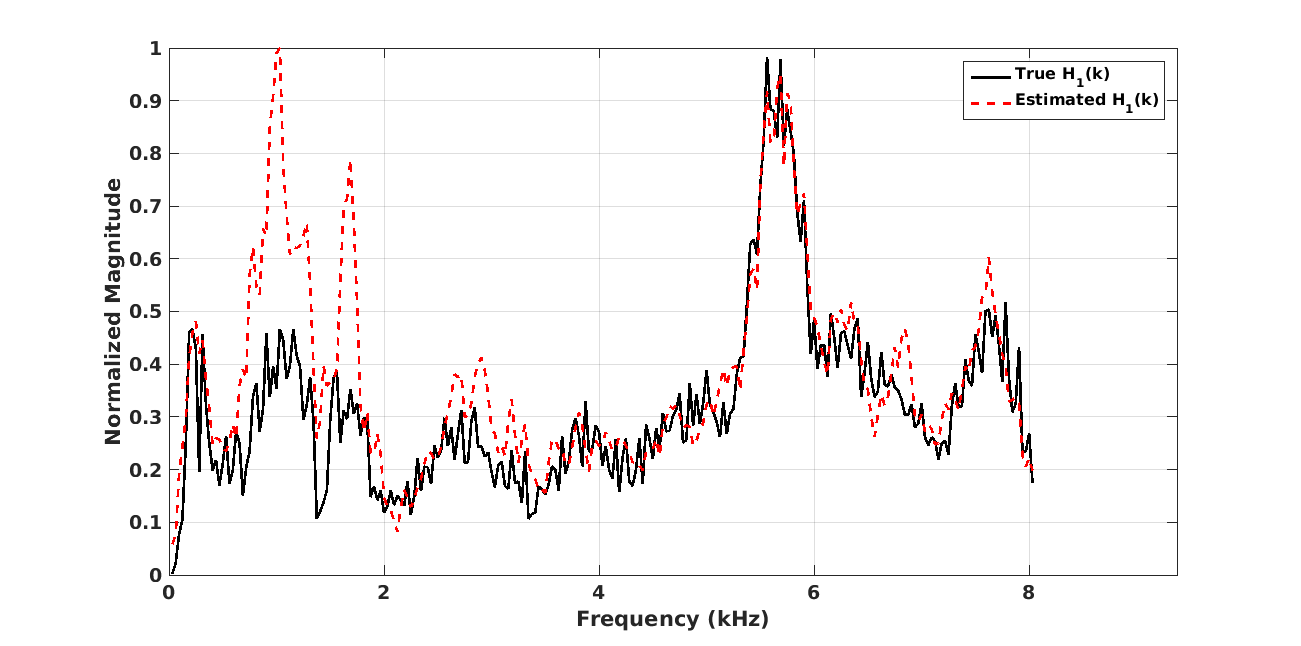
\includegraphics[width=8.2cm, height=4.5cm]{fig/freqEnv_comparison.png}
  \caption{Comparison of the estimated frequency envelope $H_1(k)$ to that of the true frequency envelope $H^{True}_1(k)$ for a measured RIR with $T_{60}\approx 700$~ms and $d=0.5$~m.}
  \label{fig:freqEnv_comp}
\end{figure}

The second step of the proposed approach can be justified by showing that the clean speech activations can be obtained from a deconvolution of the reverb activations and $H_2(k)$. Figure~\ref{fig:activation_comp} compares the activations obtained using the different NMF models for a specific basis, which is obtained from the NMF decomposition of the reverberated utterance. The clean speech activations (shown in Figure~\ref{fig:activation_comp}(a)) spread due to the effect of reverberation as is shown in Figure~\ref{fig:activation_comp}(b). Dereverberation using the proposed approach helps in reducing this effect. This is evident from the activations estimated using the R-NMF method as shown in Figure~\ref{fig:activation_comp}(d). The C-NMF+NMF method (shown in Figure~\ref{fig:activation_comp}(c)) was unable to completely recover the clean activations in this case. In our experiments, it was observed that the R-NMF consistently obtained the clean activations, whereas the C-NMF+NMF was not consistent. 
\begin{figure}[tbh!]
  \centering
  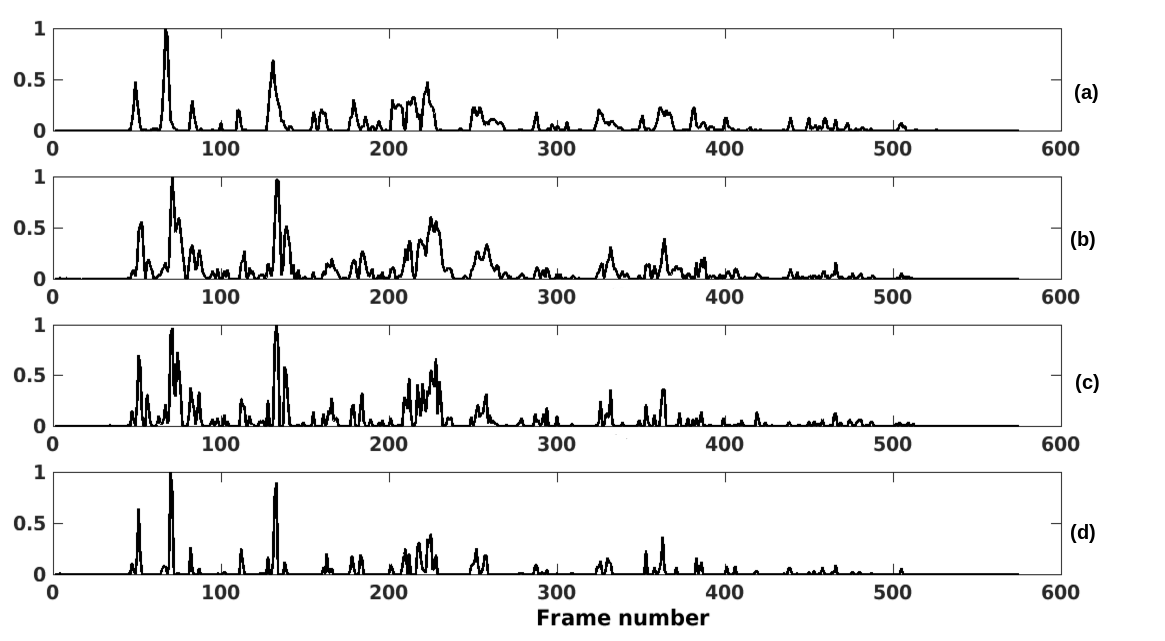
\includegraphics[width=8.5cm, height=6cm]{fig/activation_comparison4.png}
  \caption{Normalized activations obtained for a test utterance. (a) Clean utterance, (b) Reverb utterance, (c) Dereverberation using C-NMF+NMF, (d) Dereverberation using R-NMF. The estimated activations in (d) are similar to   
the true activations in (a).}
  \label{fig:activation_comp}
\end{figure}
The overall enhancement obtained using the R-NMF and C-NMF+NMF is in Figure~\ref{fig:speech_production} by comparing the enhanced spectrograms with the clean and reverb spectrograms. It can be seen that the R-NMF was more effective in removing the artifacts caused due to reverberation. This is clearly visible in the silence regions as indicated by the red boxes.
%Due to reverberations, speech spectrum spreads into the silence region. The method is able to reduce this effect.
\begin{figure}[tbh!]
  \centering
  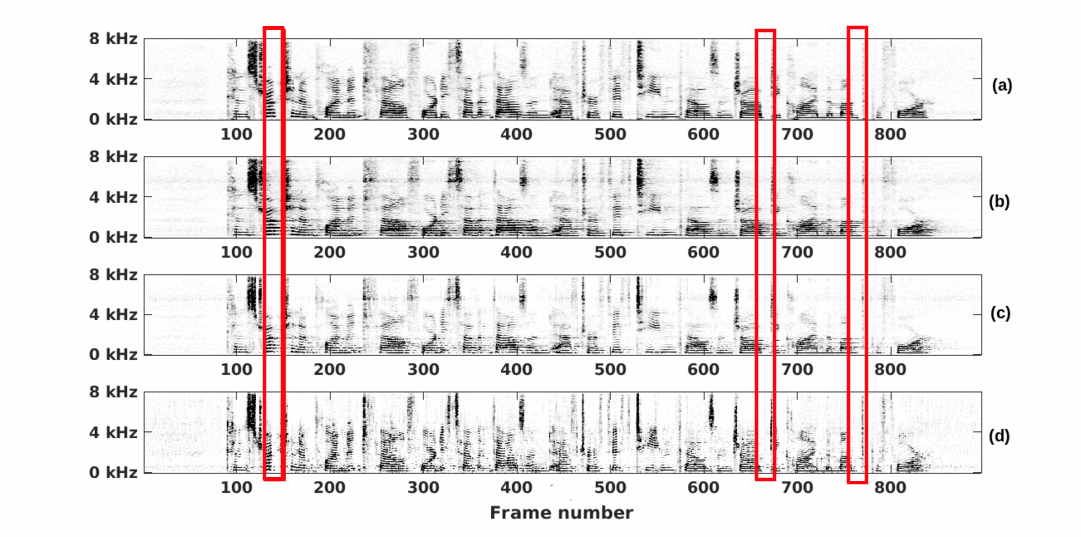
\includegraphics[width=8.5cm, height=5cm]{fig/spectrogram_prop3.png}
  \caption{Spectrogram of (a) Clean speech, (b) Reverb speech, (c) Enhanced speech using C-NMF+NMF, and (d) Enhanced speech using the proposed R-NMF. The regions where R-NMF performs better is shown using red boxes.}
  \label{fig:speech_production}
\end{figure}

%\subsection{Non-convolutive NMF model for reverberation and noise}
\subsection{Proposed model for reverberation and noise}
One of the advantages of having the NMF model for reverberation as proposed in (\ref{eq:reverbNMF}) is that it can be easily extended to include a NMF model for additive noise. The time-domain degraded speech can be represented as $y_D(t)=y(t)+z(t)$. The corresponding magnitude spectrogram $\mathbf{Y}_D$ can be approximated as the sum of reverberation spectrogram $\tilde{\mathbf{Y}}$ and noise spectrogram $\mathbf{Z}$~\cite{baby2015coupled,baby2016phd,baby2016supervised}. Further, the noise spectrogram can also be decomposed using a NMF model ($\mathbf{Z}=\mathbf{W}_n\mathbf{X}_n$)~\cite{wilson2008speech}. Hence,
\begin{align}
\tilde{Y}_D(k,n) &= \tilde{Y}(k,n)+Z(k,n) \text{,}\label{eq:NMFdeg}\\
\text{where }Z(k,r)&=\sum_{r=1}^{R_n} W_{n}(k,r)X_{n}(r,n)\text{.}
\end{align}
$\tilde{Y}_D(k,n)$, $Z(k,n)$ represent the $(k,n)$-th element of ${\tilde{\mathbf{Y}}_D}$, $\mathbf{Z}$, respectively, with $W_{n}(k,r)$ and $X_{n}(r,n)$ representing the bases and activations for the noise spectrogram and $R_n$ the rank of NMF decomposition for $\mathbf{Z}$. The model in (\ref{eq:NMFdeg}) can be written as,
\begin{align}
\tilde{\mathbf{Y}}_D = \mathbf{W}_R\mathbf{X}_R + \mathbf{W}_n\mathbf{X}_n = [\mathbf{W}_R | \mathbf{W}_n] [\mathbf{X}_R^T | \mathbf{X}_n^T]^T
\label{eq:degNMF}
\end{align}
%\begin{align}
%\tilde{\mathbf{Y}}_D &= \mathbf{W}_R\mathbf{X}_R + \mathbf{W}_n\mathbf{X}_n\nonumber \\
%& = [\mathbf{W}_R | \mathbf{W}_n] [\mathbf{X}_R^T | \mathbf{X}_n^T]^T
%\label{eq:degNMF}
%\end{align}
The bases for the decomposition are the combined bases of reverb and noise spectrograms. The reverb basis $W_R(k,r)$ depends on clean speech basis $W_s(k,r)$ as $W_R(k,r)=W_s(k,r)H_1(k)$. Activations for the decomposition in (\ref{eq:degNMF}) are the combined activations of reverberation and noise activations. The parameters $H_1(k)$, $\mathbf{X}_R$ and $\mathbf{X}_n$ are estimated using multiplicative update rules for the cost function, similar to~(\ref{eq:C}), except that $Y(n,k)$ and $\tilde{Y}(n,k)$ is replaced by $Y_D(n,k)$ and $\tilde{Y}_D(n,k)$.
%\begin{equation}
%C_D = \sum_{n,k} \bigg[Y_D(k,n)\text{ln}\bigg(\dfrac{Y_D(k,n)}{\tilde{Y}_D(k,n)}\bigg) - Y_D(k,n) + \tilde{Y}_D(k,n)\bigg]
%\end{equation}
The update rules for $H_1(k)$ and $\mathbf{X}_R$ are similar to the updates in equation (\ref{eq:updateProp}), except that $Y(k,n)$ and $\tilde{Y}(k,n)$ are replaced by $Y_D(k,n)$ and $\tilde{Y}_D(k,n)$, respectively. Update of $\mathbf{X}_n$ is obtained as,
\begin{equation}
X_n(n,r) \leftarrow X_n(n,r) \dfrac{\sum_k \dfrac{Y_D(k,n)}{\tilde{Y}_D(k,n)}W_n(k,r)}{\sum_k W_n(k,r)}
\end{equation}
We will refer to this model as R-NMF+NMF.
%Here an NMF model is assumed for the noise spectrogram.  The enhanced speech is estimated by simultaneously solving for $H(f,n)$, $X_s(r,n)$ and $X_n(r,n)$. The objective function to be minimized is a non-convex function and is liable to give unsatisfactory solution. Sparsity constrain are added to the clean and noise activations to improve the performance.

%\begin{table*}[htb]
%\centering
%\caption{Relative improvements in objective measures for the reverberant data at $20$~dB SNR.}
%\label{tab:20dB}
%\begin{tabular}{|l|l|l|l|l|l|l|l|l|l|l|l|l|ll}
%\cline{1-13}
%\multirow{2}{*}{} & \multicolumn{4}{c|}{CD}                                       & \multicolumn{4}{c|}{SRMR}                                     & \multicolumn{4}{c|}{PESQ}                                     &  &  \\ \cline{2-13}
%                  & RIR1          & RIR2          & RIR3          & RIR4          & RIR1          & RIR2          & RIR3          & RIR4          & RIR1          & RIR2          & RIR3          & RIR4          &  &  \\ \cline{1-13}
%Degraded speech   & 3.92          & 4.78          & 4.06          & 4.82          & 4.89          & 2.59          & 3.98          & 2.37          & 2.52          & 1.93          & 2.41          & 1.92          &  &  \\ \cline{1-13}
%C-NMF+NMF         & 4.27          & 4.50          & 4.39          & 4.60          & \textbf{5.71} & \textbf{4.33} & \textbf{5.62} & 4.51          & \textbf{2.74} & \textbf{2.33} & \textbf{2.69} & \textbf{2.33} &  &  \\ \cline{1-13}
%R-NMF             & \textbf{3.73} & \textbf{4.35} & 3.89          & \textbf{4.23} & 5.52          & 3.93          & 4.90          & 4.24          & 2.71          & 2.12          & 2.56          & 2.12          &  &  \\ \cline{1-13}
%R-NMF+NMF         & 3.76          & 4.53          & \textbf{3.83} & 4.47          & \textbf{5.71} & 4.14          & 5.32          & \textbf{4.26} & 2.67          & 2.00          & 2.52          & 2.00          &  &  \\ \cline{1-13}
%\end{tabular}
%\end{table*}
\begin{table*}[htb]
\centering
\caption{Comparison of objective measures for the reverberant and noisy speech, with stationary noise at $10$~dB SNR}
\label{tab:10dB}
\begin{tabular}{|l|l|l|l|l|l|l|l|l|}
\hline
\multirow{2}{*}{} & \multicolumn{4}{c|}{CD}                                       & \multicolumn{4}{c|}{SRMR}                                     \\ \cline{2-9} 
                  & RIR1          & RIR2          & RIR3          & RIR4          & RIR1          & RIR2          & RIR3          & RIR4          \\ \hline
Degraded speech   & 4.98          & 5.43          & 5.07          & 5.46          & 3.24          & 2.08          & 3.03          & 1.92          \\ \hline
C-NMF+NMF~\cite{mohammadiha2016speech,Mohammadiha2015}         & 5.28          & 5.35          & 5.38          & 5.45          & 4.69          & 3.71          & 4.70          & 3.85          \\ \hline
R-NMF             & 4.85          & 5.16          & 4.97          & 5.26          & 4.16          & 3.43          & 3.99          & 3.73          \\ \hline
R-NMF+NMF          & \textbf{4.40} & \textbf{4.49} & \textbf{4.49} & \textbf{4.48} & \textbf{5.37} & \textbf{4.08} & \textbf{5.20} & \textbf{4.12} \\ \hline
\end{tabular}
\end{table*}
%\begin{table*}[htb]
%\centering
%\caption{Relative improvements in objective measures for the reverberant data at $10$~dB SNR.}
%\label{tab:10dB}
%\begin{tabular}{|l|l|l|l|l|l|l|l|l|l|l|l|l|ll}
%\cline{1-13}
%\multirow{2}{*}{} & \multicolumn{4}{c|}{CD}                                       & \multicolumn{4}{c|}{SRMR}                                     & \multicolumn{4}{c|}{PESQ}                                     &  &  \\ \cline{2-13}
%                  & RIR1          & RIR2          & RIR3          & RIR4          & RIR1          & RIR2          & RIR3          & RIR4          & RIR1          & RIR2          & RIR3          & RIR4          &  &  \\ \cline{1-13}
%Degraded speech   & 4.98          & 5.43          & 5.07          & 5.46          & 3.24          & 2.08          & 3.03          & 1.92          & 2.09          & 1.73          & 2.06          & 1.73          &  &  \\ \cline{1-13}
%C-NMF+NMF         & 5.28          & 5.35          & 5.38          & 5.45          & 4.69          & 3.71          & 4.70          & 3.85          & 2.24          & \textbf{2.01} & \textbf{2.24} & \textbf{2.06} &  &  \\ \cline{1-13}
%R-NMF             & 4.85          & 5.16          & 4.97          & 5.26          & 4.16          & 3.43          & 3.99          & 3.73          & 2.15          & 1.85          & 2.08          & 1.86          &  &  \\ \cline{1-13}
%R-NMF+NMF         & \textbf{4.40} & \textbf{4.49} & \textbf{4.49} & \textbf{4.48} & \textbf{5.37} & \textbf{4.08} & \textbf{5.20} & \textbf{4.12} & \textbf{2.31} & 1.81          & 2.20          & 1.89          &  &  \\ \cline{1-13}
%\end{tabular}
%\end{table*}
\begin{table*}[hbt]
\centering
\caption{Comparison of objective measures for the reverberant and noisy speech, with non-stationary noise (Factory) at $10$~dB SNR}
\label{tab:10dBnonStat}
\begin{tabular}{|l|l|l|l|l|l|l|l|l|}
\hline
\multirow{2}{*}{} & \multicolumn{4}{c|}{CD}                                       & \multicolumn{4}{c|}{SRMR}                                     \\ \cline{2-9} 
                  & RIR1          & RIR2          & RIR3          & RIR4          & RIR1          & RIR2          & RIR3          & RIR4          \\ \hline
Degraded speech   & 5.28          & 5.63          & 5.36          & 5.68          & 3.53          & 2.22          & 3.25          & 2.05          \\ \hline
C-NMF+NMF~\cite{mohammadiha2016speech,Mohammadiha2015}         & 5.60          & 5.65          & 5.75          & 5.82          & 4.81          & 3.83          & 4.83          & 3.99          \\ \hline
R-NMF             & 5.16          & 5.43          & 5.28          & 5.55          & 4.50          & 3.53          & 4.30          & 3.84          \\ \hline
R-NMF+NMF          & \textbf{4.77} & \textbf{5.12} & \textbf{4.80} & \textbf{5.17} & \textbf{5.50} & \textbf{4.32} & \textbf{5.15} & \textbf{4.31} \\ \hline
\end{tabular}
\end{table*}
%\begin{table*}[hbt]
%\centering
%\caption{Relative improvements in objective measures for the reverberant data for non-stationary noise (Factory) added at $10$~dB SNR.}
%\label{tab:10dBnonStat}
%\begin{tabular}{|l|l|l|l|l|l|l|l|l|l|l|l|l|ll}
%\cline{1-13}
%\multirow{2}{*}{} & \multicolumn{4}{c|}{CD}                                       & \multicolumn{4}{c|}{SRMR}                                     & \multicolumn{4}{c|}{PESQ}                                     &  &  \\ \cline{2-13}
%                  & RIR1          & RIR2          & RIR3          & RIR4          & RIR1          & RIR2          & RIR3          & RIR4          & RIR1          & RIR2          & RIR3          & RIR4          &  &  \\ \cline{1-13}
%Degraded speech   & 5.28          & 5.63          & 5.36          & 5.68          & 3.53          & 2.22          & 3.25          & 2.05          & 2.15          & 1.74          & 2.10          & 1.75          &  &  \\ \cline{1-13}
%C-NMF+NMF         & 5.60          & 5.65          & 5.75          & 5.82          & 4.81          & 3.83          & 4.83          & 3.99          & \textbf{2.28} & \textbf{2.03} & \textbf{2.26} & \textbf{2.05} &  &  \\ \cline{1-13}
%R-NMF             & 5.16          & 5.43          & 5.28          & 5.55          & 4.50          & 3.53          & 4.30          & 3.84          & 2.22          & 1.86          & 2.13          & 1.88          &  &  \\ \cline{1-13}
%R-NMF+NMF         & \textbf{4.77} & \textbf{5.12} & \textbf{4.80} & \textbf{5.17} & \textbf{5.50} & \textbf{4.32} & \textbf{5.15} & \textbf{4.31} & 2.25          & 1.76          & 2.19          & 1.74          &  &  \\ \cline{1-13}
%\end{tabular}
%\end{table*}
\section{Results}
The performance of the algorithms in Sec. 2 was compared using speech enhancement measures. As mentioned earlier, we do not consider~\cite{baby2015coupled, baby2016phd, baby2017joint} as these are exemplar based methods.

\subsection{Dataset and experiments}
%The speech enhancement performance was compared using the TIMIT database \cite{garofolo1993timit}.
The speech enhancement performance was assessed using a subset of $16$ speakers, with ten utterances per speaker from the TIMIT database~\cite{garofolo1993timit}. One utterance spoken by each speaker was used for testing.
%A subset of $16$ different sentences spoken by $16$ distinct speakers was used for testing. 
For the NMF representation, $100$ speaker specific clean speech bases were learned from $9$ utterances different from the one used in testing of that speaker.
Four measured RIRs from the REVERB challenge \cite{kinoshita2016summary} were used for the evaluation. The RIRs correspond to two different rooms and two different source-microphone distances : near ($0.5$~m) and far ($2$~m) in each room. RIR1 and RIR2 correspond to near and far RIR recordings in the room with $T_{60}\approx600$~ms. RIR3 and RIR4 correspond to near and far RIR recordings for the room with $T_{60}\approx700$~ms. 
Each test sentence was convolved with these RIRs to obtain a total of 64 reverberated recordings. 
Stationary noise available from REVERB challenge~\cite{kinoshita2016summary} or non-stationary noise (factory noise) from~\cite{varga1993assessment} was added to the reverberant data at different signal-to-noise ratios (SNRs). $100$ noise bases were learned from these noise recordings.

The magnitude spectrogram of the $64$ reverberant signals was obtained using a $64$~ms window with a hop-size of $16$~ms. The square root of Hanning window was used in analysis and synthesis. $L_h$ in (\ref{eq:deg2}) was experimentally fixed as $40$. $H_1(k)$ was initialized to $1$ for all $k$, $\mathbf{X}_R$ and $\mathbf{X}_n$ were initialized to random values.
% and $H_2(n)$ was obtained assuming the knowledge of RIR. $H_2(n)$ was obtained as the average of $H(n,k)$ for different subbands. Each subband is normalized to have a maximum value $1$. 
With the knowledge of RIR, $H_2(n)$ was obtained as the average of $H(n,k)$ for different subbands. Each subband is normalized to have a maximum value $1$.
The enhanced speech is reconstructed using original noisy phase.
The improvement in speech enhancement task was compared using the objective measures of CD and SRMR~\cite{hu2008evaluation, falk2010non}. Note, we do not include PESQ as it does not provide consistent estimates, as observed in~\cite{kinoshita2016summary}. Dereverberated speech has larger SRMR scores and lower CD when compared to the reverberated speech. The performance of the algorithms is reflected in these measures.
%The magnitude spectrogram in (\ref{eq:deg2}) was obtained using $L_h=40$. 
%$H_2(n)$ as an exponentially decaying function with the rate of decay obtained from knowledge of room and source-microphone distance. 
%was a exponentially decaying function with the rate of decay fixed from knowledge of similar RIRs. $100$ iterations are performed for each algorithm is performed to obtain these parameters. The estimated clean speech spectrogram was obtained using phase spectrogram of degraded signal.
%Each narrowband H k was initialized as a linearly decreasing function, and S was initialized using the spectrogram of reverberated speech. For algorithms with speech model, initial values for the basis and the activations were obtained by performing NMF decomposition on the spectrogram of reverberated speech. Since the algorithms converge fast, 20 iterations are performed for each algorithm to obtain the estimates of Ŝ and Ĥ.
\subsection{Speech enhancement using the proposed methods}
The performance of the proposed algorithms was compared to the C-NMF+NMF method, for the various reverberation conditions with stationary or non-stationary noise added at different SNRs. For want of space, we do not include the results for $20$~dB noise where all the methods behave similarly, with R-NMF+NMF performing slightly better. Table~\ref{tab:10dB} provides objective measures for the degraded speech with a stationary noise at $10$~dB SNR and the enhanced speech obtained using the various methods.  
%Table~\ref{tab:10dB} compares relative improvements in objective measures obtained by the algorithms for the reverb data and stationary noise at $10$~dB SNR. 
It can be seen that R-NMF enhanced speech shows improvement in all the objective measures. 
%However, the relative improvements are less when compared with the C-NMF+NMF. 
Considering SRMR, the performance of C-NMF+NMF and R-NMF methods are comparable. However, R-NMF leads to improvements in CD, whereas C-NMF+NMF results in poor CD. The R-NMF+NMF provides significantly better improvements in both the measures when compared to C-NMF+NMF. 
% The reason for this can be that the R-NMF is based on a simplifying separability assumption on RIR spectrogram ($H(n,k)$). Introducing noise model for the proposed approach (R-NMF+NMF) also did not improve the performance. This may be due to the less noisy condition. 
%The performance of the proposed algorithms was compared to two dereverberation algorithms, C-NMF and C-NMF with speech model (C-NMF+NMF) [5], for 4 different reverberation conditions. Initially the comparison was based on SRMR improvements and is shown in Table 1. As observed in Fig. 1 and Sec. 3.4 the RIR regularization on C-NMF does not improve the RIR estimates, and hence the SRMR does not improve in these cases (Rows 1, 2, 3 in Table 1). However, similar regularization on C-NMF+NMF resulted in better RIR estimates and leads to SRMR improvements (Rows 4, 5 in Table 1). Among the RIRs considered, since the SRMR improvement was significant for RIR 1 , other objective measures for RIR 1 were also considered and this is shown in Table 2. It can be observed from Table 2 that the baseline dereverberation algorithms C-NMF and C-NMF+NMF are able to enhance the reverberated speech. Inducing sparsity (C-NMF+H sparse ) or frequency envelope on H (C-NMF+H gain ) does not improve performance. The reason for the sparse H sparse showing no improvement could be that narrow band H roughly has the exponentially decaying structure which we hope to achieve. The multiplicative update for the cost function in (9) is obtained such that it minimizes the error in each narrowband independently. Hence, effectively the cost-function remains the same even after having a frequency envelope on H. All the objective measures show improvement for C-NMF+H early . Both, C-NMF+NMF+H sparse and C-NMF+NMF+H early show significant improvements in SRMR, and other measures change marginally. One possible explanation can be that the regularization reduces reverberation, but also adds distortion to the dereverberated speech.

Table~\ref{tab:10dBnonStat} compares the enhancement results obtained using the proposed methods when non-stationary (factory) noise is added at $10$~dB SNR. It can be seen that the R-NMF method performs relatively better compared to C-NMF+NMF. Here too the proposed R-NMF+NMF based enhancement significantly improved the performance, as is evident from the CD and SRMR improvements.

%Table~\ref{tab:10dB} compare the relative improvements in objective measures obtained at $10$~dB noise. 
In the presence of noise, the enhancement performance of C-NMF+NMF and R-NMF are comparable, which is expected as there is no explicit model for noise. But, this also shows that the proposed non-convolutive NMF model for dereverberation is equivalent to existing C-NMF model. 
%R-NMF model perform better as seen the objective measures. 
%With the introduction of noise model, the proposed method performance is significantly improved. This can be observed in CD and SRMR improvements. 
\section{Discussion and Summary}
The proposed R-NMF and R-NMF+NMF methods model reverberation using a non-convolutive NMF model. Assuming a NMF model for noise, R-NMF+NMF method jointly handles noise and reverberation. Such a method provides improved speech enhancement compared to a C-NMF model that does not handle noise. Further, the enhancement results for R-NMF	demonstrates the effectiveness of using a NMF model to perform dereverberation. 
This leads to simple updates and less computational complexity. 
In addition, using the proposed model we also showed a convincing interpretation of the effects of reverberation on the clean speech activations.  
%Such a representation leads to a model where noise can be handled efficiently. This mode provide significant enhancement in a noisy and reverberant environment. 
The NMF based methods proposed here used learned bases for each speaker. As part of future work, we will look at incorporating speaker independent and exemplar bases. The improvements in CD and SRMR indicate that the proposed method will lead to improved single-channel ASR systems for reverberant and noisy conditions.
%The method is shown to work when speaker specific bases are used. The performance needs to be evaluated when speaker independent bases is used. The algorithm should also need to be checked for automatic speech recognition (ASR) performance.
%\section{Conclusions}
%A dereverberation algorithm using conventional NMF as opposed to CNMF mode was introduced in this paper. This dereverberation method was shown to improve the speech enhancement measures. Another advantage of having this method is that such a method can directly incorporate NMF model for noise, and the combined degradation can be viewed as another NMF mode with bases and activations to represent reverberation and noise. Such an approach has shown to significantly improve the enhancement result as compared to the baseline method (C-NMF+NMF). 

\fi
\chapter{Low-rank NMF model for RIR spectrogram}
\label{chapter:trans2020}

\section{Justification of low-rank approximation}
\begin{itemize}
\item Quality of approximation
\item generalization of separability approximation
\begin{itemize}
\item remove limitations of earlier work
\item easy to interpret model
\end{itemize}
\end{itemize}

\section{NMF model for degraded spectrogram}
\begin{itemize}
\item derivation of NMF model for reverb and degraded spectrogram
\item comparison of degradation model obtained with proposed method when compared with NMF based methods in literature
\item effect of clean speech bases and activation with reverberation
\end{itemize}

\section{Algorithm details}
\begin{itemize}
\item cost function
\item multiplicative update rule
\end{itemize}

\section{Experimental results}
\begin{itemize}
\item enhancement results, ASR results
\item variation of performance with RIR, SNR, rank of decomposition, etc.
\end{itemize}

\begin{table}[]
\centering
\begin{tabular}{|l|c|}
\hline
\multicolumn{1}{|c|}{\textbf{Method}} & \textbf{WER (\%)} \\ \hline
Clean                                 & 3.44              \\ \hline
Degraded                              & 62.34             \\ \hline
CNMF0                                 & 47.95             \\ \hline
CNMF1\_s                              & 44.45             \\ \hline
CNMF2\_s                              & 43.24             \\ \hline
RNMF\_s                               & \textbf{40.24}    \\ \hline
\end{tabular}
\caption{Enhancement results when reverberated with RIR \text{RIR3\_far} and stationary noise added with $10$~dB SNR. The RIR has $T_{60}\approx 700$~ms and source-microphone distance of $2$~m. }
\end{table}

\begin{table}[]
\centering
\begin{tabular}{|l|c|l|l|l|}
\hline
\multicolumn{1}{|c|}{\textbf{Method}}                                                         & \multicolumn{4}{c|}{\textbf{WER (\%)}}                                                                                                     \\ \hline
Clean                                                                                         & \multicolumn{4}{c|}{3.44}                                                                                                                  \\ \hline
\multirow{2}{*}{\textbf{\begin{tabular}[c]{@{}l@{}}Degradation \\ condition\end{tabular}}} & \textbf{R2\_near} & \multicolumn{1}{c|}{\textbf{R2\_far}} & \multicolumn{1}{c|}{\textbf{R3\_near}} & \multicolumn{1}{c|}{\textbf{R3\_far}} \\ \cline{2-5} 
                                                                                              &                   & \multicolumn{1}{c|}{48.57}            & \multicolumn{1}{c|}{19.41}             & \multicolumn{1}{c|}{62.34}            \\ \hline
CNMF0                                                                                         &                   &                                       &                                        & 47.95                                 \\ \hline
CNMF1\_s                                                                                      &                   &                                       &                                        & 44.45                                 \\ \hline
CNMF2\_s                                                                                      &                   &                                       &                                        & 43.24                                 \\ \hline
RNMF\_s                                                                                       &                   &                                       &                                        & \textbf{40.24}                        \\ \hline
\end{tabular}
\caption{Enhancement results for $10$~dB SNR stationary noise.}
\end{table}

\begin{table}[]
\centering
\begin{tabular}{|l|c|l|l|l|}
\hline
\multicolumn{1}{|c|}{\textbf{Method}}                                                         & \multicolumn{4}{c|}{\textbf{WER (\%)}}                                                                                                     \\ \hline
Clean                                                                                         & \multicolumn{4}{c|}{3.44}                                                                                                                  \\ \hline
\multirow{2}{*}{\textbf{\begin{tabular}[c]{@{}l@{}}Degradation \\ condition\end{tabular}}} & \textbf{R2\_near} & \multicolumn{1}{c|}{\textbf{R2\_far}} & \multicolumn{1}{c|}{\textbf{R3\_near}} & \multicolumn{1}{c|}{\textbf{R3\_far}} \\ \cline{2-5} 
                                                                                              &                   & \multicolumn{1}{c|}{}            & \multicolumn{1}{c|}{}             & \multicolumn{1}{c|}{}            \\ \hline
CNMF0                                                                                         &                   &                                       &                                        &                                  \\ \hline
CNMF1\_s                                                                                      &                   &                                       &                                        &                                  \\ \hline
CNMF2\_s                                                                                      &                   &                                       &                                        &                                  \\ \hline
RNMF\_s                                                                                       &                   &                                       &                                        &                         \\ \hline
\end{tabular}
\caption{Enhancement results for $20$~dB SNR stationary noise.}
\end{table}

\begin{table}[]
\centering
\begin{tabular}{|l|c|l|l|l|}
\hline
\multicolumn{1}{|c|}{\textbf{Method}}                                                         & \multicolumn{4}{c|}{\textbf{WER (\%)}}                                                                                                     \\ \hline
Clean                                                                                         & \multicolumn{4}{c|}{3.44}                                                                                                                  \\ \hline
\multirow{2}{*}{\textbf{\begin{tabular}[c]{@{}l@{}}Degradation \\ condition\end{tabular}}} & \textbf{R2\_near} & \multicolumn{1}{c|}{\textbf{R2\_far}} & \multicolumn{1}{c|}{\textbf{R3\_near}} & \multicolumn{1}{c|}{\textbf{R3\_far}} \\ \cline{2-5} 
                                                                                              &                   & \multicolumn{1}{c|}{}            & \multicolumn{1}{c|}{}             & \multicolumn{1}{c|}{}            \\ \hline
CNMF0                                                                                         &                   &                                       &                                        &                                  \\ \hline
CNMF1\_s                                                                                      &                   &                                       &                                        &                                  \\ \hline
CNMF2\_s                                                                                      &                   &                                       &                                        &                                  \\ \hline
RNMF\_s                                                                                       &                   &                                       &                                        & \textbf{}                        \\ \hline
\end{tabular}
\caption{Enhancement results for noise free condition.}
\end{table}

\section{Discussion}

\iffalse
\section{Introduction}
Speech originating from a source undergoes multiple reflections in a closed room. When this speech is captured using a microphone distant from the source (typically 30 cm to few meters), the microphone output is a superposition of the speech along with the delayed and attenuated copies of the signal referred to as reverberated speech~\cite{naylor2010speech}. Additionally, the microphone will capture background noise originating from other sources. The resulting microphone output in such a distant speech recording (DSR) setting is a degraded version of the original speech signal. The presence of such degradations impedes speech intelligibility~\cite{kinoshita2016summary}  and automatic speech recognition (ASR)~\cite{barker2018fifth, barker2015third} performance. The amount of degradation depends on the source and microphone positions, characteristics of the room and the noise~\cite{naylor2010speech,kinoshita2016summary}. To improve performance, it is desirable to compensate for these degradations. The focus of this work is on jointly handling dereverberation and denoising. In this work we refer to methods that perform dereverberation in presence of noise as speech enhancement methods.

Dereverberation methods in literature can be broadly classified as (i) beamforming methods, (ii) inverse filtering methods and (iii) reverberation suppression methods. Many of these approaches can be extended to jointly handle reverberation and noise. (i) Beamforming is a multi-channel method. It uses a spatial filter that enhances speech incident from the desired direction and suppresses speech coming from other directions~\cite{gannot2017consolidated}. 
%The multi-channel recordings are filtered and weighed to focus the beam to the desired direction. 
(ii) Inverse filtering methods blindly estimate the room impulse response (RIR) from the microphone recordings. Blind system identification approaches like the least-squares (LS) method and eigendecomposition method are used to blindly estimate the RIR~\cite{naylor2010speech}. This RIR is used to retrieve the original speech source. (iii) Reverberation suppression methods model the effect of reverberation on the clean speech in some domains like the short-time Fourier transform (STFT), the residual signal obtained from linear prediction analysis, etc. Based on these models, algorithms are proposed to reduce the effects of reverberation. This results in a better estimate of clean speech. The approaches include spectral subtraction~\cite{lebart2001new}, weighted linear prediction (WPE)~\cite{nakatani2010speech}, Triple-N ICA for convolutive mixtures (TRINICON)~\cite{buchner2007trinicon}, linear prediction based method~\cite{naylor2010speech}, and NMF based approaches~\cite{kameoka2009robust}, etc. In this work, a novel single-channel NMF based method to perform dereverberation and denoising jointly is proposed. Various NMF based enhancement methods proposed in literature are discussed next. 

NMF based dereverberation methods are based on the non-negative convolutive transfer function (N-CTF) model for the magnitude STFT of the reverberated speech ~\cite{kameoka2009robust,mohammadiha2016speech, Mohammadiha2015, Kumar2011}. For each frequency band, the temporal variation of reverberated speech is modeled as the convolution of magnitude spectrogram values of the clean speech and the RIR for that particular frequency. This model is valid when the reverberation condition does not change with time. Further, the N-CTF model is obtained by ignoring the cross-band effects occurring due to windowing~\cite{avargel2007system}.  Even though these approximations in the N-CTF model can pose a limitation for the dereverberation task, many dereverberation methods use this model. An additional advantage of the N-CTF model is that it avoids the need for a phase estimate of the RIR. Obtaining the phase spectrogram is difficult, especially if the recording is noisy~\cite{kameoka2009robust}. 

Based on the N-CTF model, a speech dereverberation algorithm was proposed in~\cite{kameoka2009robust}. Estimation of clean speech spectrogram is viewed as solving a CNMF problem. This algorithm shows improvements in speech enhancement instrumental measures. In~\cite{Kumar2011}, the N-CTF model for reverberation is extended for a gammatone filterbank. The estimated clean speech features are shown to improve ASR performance. In~\cite{Kallasjoki2014}, a NMF model for speech reverberation is proposed which is equivalent to the CNMF model for reverberation. The bases matrix of the NMF decomposition is a structured matrix that mimics the CNMF model. 
The dereverberation performance using the CNMF model was improved by introducing models for clean speech spectrograms like NMF~\cite{mohammadiha2016speech, Mohammadiha2015} and CNMF~\cite{Mirsamadi2014} models. Many constraints on the estimated clean speech are used such as sparsity~\cite{mohammadiha2016speech, Mohammadiha2015} and continuity~\cite{wager2018collaborative} to improve the performance.

The N-CTF model cannot be used as such for reverberated speech in the presence of noise. Including a noise model to the N-CTF model helps in improving the dereverberation performance. The magnitude spectrogram of reverberated speech in the presence of noise is approximated as the sum of magnitude spectrograms of reverberated speech and noise~\cite{li2018multichannel}. Using this model, along with NMF models for clean speech and noise spectrograms, a supervised joint dereverberation and denoising algorithm was proposed in~\cite{baby2016supervised}. The use of the CNMF model for the clean speech and the noise spectrogram was also proposed in~\cite{baby2016supervised, baby2016phd}. All the enhancement methods based on N-CTF discussed above use models for clean speech spectrogram, but do not use any specific models for the RIR spectrogram.

Use of meaningful constraints on the RIR spectrogram along with speech model will help the dereverberation methods. Some methods use a simple model for the RIR spectrogram. The temporal variation of the RIR spectrogram was modeled in~\cite{baby2016supervised}. The RIR spectrogram energy across frames was modeled to decay with time. Based on this RIR model, an enhancement algorithm was proposed in~\cite{baby2017joint}, to improve the speech enhancement results. This method does not consider the spectral variation of the RIR spectrogram. With the knowledge of the RIR, we had proposed in~\cite{mohanan2017speech}, the use of the sparse nature and the presence of a frequency envelope for the RIR spectrogram to improve the speech enhancement results. Further, in~\cite{mohanan201a}, a spectral and temporal model for the RIR spectrogram was proposed based on a separability approximation on the RIR spectrogram. The approximation resulted in a rank-$1$ NMF model for the RIR spectrogram. Based on the RIR model, the reverberated speech spectrogram was modeled using NMF as opposed to CNMF model used in literature.

In this work, we propose a NMF based approach to handle dereverberation and denoising jointly. Such an approach is different from other NMF based approaches that use a combination of CNMF and NMF for the purpose. The proposed model is easy to interpret. The spectral and temporal variation of the RIR is modeled using a low-rank NMF approximation of the RIR spectrogram. Even though such a representation reduces the number of parameters used for representing the RIR spectrogram, the enhancement results obtained are better than other NMF based approaches. Further, the approach is extended to work in unknown noise conditions. Such an approach gives better enhancement results when compared to existing NMF based dereverberation methods. More importantly the RIR spectrogram estimate obtained using the proposed approach is better and closer to the true RIR spectrogram when compared to estimates from other NMF based approaches.

The main contribution of this paper is in proposing and incorporating a novel spectro-temporal model for the RIR spectrogram in the N-CTF model for reverberation. This model results in a NMF based algorithm to jointly handle dereverberation and denoising. Such a representation helps in imposing better constraints on the RIR spectrogram, which was not possible in other NMF based methods. This resulted in superior enhancement results when compared to competing methods.
%The proposed algorithm showed superior enhancement results. 
This also resulted in a RIR estimate which is closer to the true RIR spectrogram.

Section~\ref{sec:deg_model} describes existing N-CTF model for reverberation and its modifications when NMF model for clean speech and noise are incorporated. Section~\ref{sec:ProposedModel} describes the proposed low-rank NMF approximation of RIR spectrogram and the resulting NMF model for reverberation and noise. 
The implementation details of the proposed algorithm are given in Section~\ref{sec:cost_fn}. This includes a description of the proposed cost function, the NMF update rules and the initialization used. In Section~\ref{sec:experiment} the experiment setup and the results are described and compared. The implicit constraint on RIR spectrogram obtained for the proposed approach is also discussed.

\section{Reverberation models using CNMF}
\label{sec:deg_model}
The initial part of the section presents the existing reverberation models based on CNMF representation of the magnitude spectrogram of reverberated speech. Extending the CNMF  model to accommodate noise is explained in the latter part.

\subsection{CNMF models for reverberated speech}
Reverberated speech $y_R(t)$ recorded at a microphone is expressed as the convolution of clean speech $s(t)$ and the RIR $h(t)$~\cite{naylor2010speech}. %\textbf{[($y(t)=s(t)*h(t)$)]}~\cite{naylor2010speech}.
%\begin{equation}
%y(t) = h(t) * s(t)
%\label{eq:deg1}
%\end{equation}
%In the magnitude spectrogram domain, the degradation is approximated as the sum of spectrograms due to reverberation and noise. 
%\subsection{C-NMF model for reverberation}
In the absence of noise, speech degradation due to reverberation can be modeled in the magnitude spectrogram domain by utilizing the modulation transfer function (MTF) model for reverberation~\cite{kameoka2009robust}. According to the MTF  model, the magnitude envelope for each subband of the reverberant speech magnitude spectrogram $\mathbf{Y}_R \in \mathbb{R}^{K \times T}_{+}$ can be approximated as the convolution of the corresponding subband magnitude envelopes of the RIR $\mathbf{H} \in \mathbb{R}^{K \times L_h}_{+}$ and the clean speech $\mathbf{S} \in \mathbb{R}^{K \times (T-L_h +1)}_{+}$ spectrograms~\cite{Kumar2011}. Accordingly, 
\begin{equation}
Y_R(k,n) \approx H(k,n)*_{\text{n}} S(k,n)=\sum_{l=0}^{L_h-1}H(k,l)S(k,n-l)\text{,}
\label{eq:deg2}
\end{equation}
where $Y_R(k,n)$, $H(k,n)$, and $S(k,n)$ represent the $(k,n)$-th element of $\mathbf{Y}_R$, $\mathbf{H}$, and $\mathbf{S}$, respectively. $L_h$ represents the number of frames used to represent the RIR spectrogram $\mathbf{H}$ and $*_{\text{n}}$ represents convolution across the frame index. The model in~(\ref{eq:deg2}) can be viewed as a CNMF decomposition where $\mathbf{H}$ and $\mathbf{S}$ can be obtained using multiplicative updates~\cite{kameoka2009robust}. We refer this method as CNMF0.

%The model in (\ref{eq:deg2}) was improved in \cite{mohammadiha2016speech,Mohammadiha2015} to use a NMF model for speech spectrogram. 
The model in (\ref{eq:deg2}) was improved by incorporating a NMF model for the magnitude spectrogram of clean speech~\cite{mohammadiha2016speech,Mohammadiha2015}.
A NMF decomposition for clean speech spectrogram $\mathbf{S}$ is,
\begin{align}
\mathbf{S}&\approx \mathbf{W}_{\text{s}} \mathbf{X}_{\text{s}}\nonumber\\
S(k,n)&\approx\sum_{r=1}^{R_{\text{s}}} W_{\text{s}}(k,r)X_{\text{s}}(r,n)\text{,}
\label{eq:nmf1}
\end{align}
where $\mathbf{W}_{\text{s}}\in \mathbb{R}_+^{K \times R_s}$ and $\mathbf{X}_{\text{s}}\in \mathbb{R}_+^{R_s \times (T-L_h +1)}$ represent the bases and activation matrix for the NMF decomposition on the clean speech spectrogram. $W_{\text{s}}(k,r)$, $X_{\text{s}}(r,n)$ are elements of the $\mathbf{W}_{\text{s}}$, $\mathbf{X}_{\text{s}}$ and $R_\text{s}$ is the rank of the decomposition. Using (\ref{eq:nmf1}) in (\ref{eq:deg2}),
\begin{equation}
Y_R(k,n) \approx \sum_{l=0}^{L_h-1}H(k,l)\bigg(\sum_{r=1}^{R_{\text{s}}} W_{\text{s}}(k,r)X_{\text{s}}(r,n-l)\bigg)\text{.}
\label{eq:deg4}
\end{equation}
From (\ref{eq:deg4}), enhanced speech is obtained by solving for $H(k,l)$, $W_{\text{s}}(k,r)$ and $X_{\text{s}}(r,n)$ iteratively. In \cite{mohammadiha2016speech,Mohammadiha2015}, several approaches to obtain bases are experimented with. In online (unsupervised) methods, the bases are learned from the reverberant speech.
%and we will refer to this method as $\text{CNMF1\_u}$. 
In offline (supervised) methods, the bases are learned from available clean speech utterances. The supervised method is used for comparison in this work and we will refer to this method as $\text{CNMF1\_s}$. 
%The proposed approach uses supervised bases, so we use the offline method as a baseline for comparison. 

\subsection{Extended model to handle noise}
In the presence of noise, the time-domain degraded speech $y(n)$ is modeled as the sum of reverberated speech $y_R(t)$ and additive noise $z(t)$. The time-domain model can be summarized as
\begin{equation}
y(t)=y_R(t)+z(t) = h(t)*s(t)+z(t),
\label{eq:time_domain_model}
\end{equation} 
where * represents the time-domain convolution. In the magnitude spectrogram domain, the degraded spectrogram can be approximated as the sum of magnitude spectrograms of reverberated speech and noise ($\mathbf{Z}\in \mathbb{R}_+^{K \times T}$)~\cite{baby2015coupled, baby2016phd, baby2017joint}. Based on this model and using (\ref{eq:deg2}), the spectrogram of degraded speech $\mathbf{Y}\in \mathbb{R}_+^{K \times T}$ can be represented as, 
\begin{align}
\mathbf{Y}&\approx \mathbf{Y}_R + \mathbf{Z}\nonumber\\
Y(k,n)&\approx Y_R(k,n) + Z(k,n) \nonumber\\
      &= H(k,n)*_{\text{n}} S(k,n)+Z(k,n),
\label{eq:deg_model1}
\end{align}
where $Y(k,n)$ and $Z(k,n)$ represent the $(k,n)$-th elements of $\mathbf{Y}$ and $\mathbf{Z}$, respectively. In~\cite{baby2015coupled}, a supervised approach based on this model to jointly handle reverberation and noise was proposed. The model utilizes NMF decomposition for the spectrograms of clean speech $\mathbf{S}$ and noise $\mathbf{Z}$. NMF decomposition of clean speech spectrogram is as shown in (\ref{eq:nmf1}). Similarly, a NMF decomposition for the noise spectrogram can be obtained as,
\begin{align}
\mathbf{Z}&\approx \mathbf{W}_{\text{n}} \mathbf{X}_{\text{n}}\nonumber\\
Z(k,n)&\approx\sum_{r=1}^{R_{\text{n}}} W_{\text{n}}(k,r)X_{\text{n}}(r,n)\text{,}
\label{eq:nmf2}
\end{align}
where $\mathbf{W}_{\text{n}}\in \mathbb{R}_+^{K \times R_{\text{n}}} \text{, }  \mathbf{X}_{\text{n}}\in \mathbb{R}_+^{R_{\text{n}} \times T}$ represent the noise bases and activation matrix, respectively. $R_{\text{n}}$ represents the rank of NMF decomposition. $W_{\text{n}}(k,r) \text{, } X_{\text{n}}(r,n)$ represent the elements of $\mathbf{W}_{\text{n}}\text{, }\mathbf{X}_{\text{n}}$, respectively. Substituting (\ref{eq:nmf1}) and (\ref{eq:nmf2}) in (\ref{eq:deg_model1}), the degraded spectrogram can be rewritten as
\begin{align}
\mathbf{Y}&\approx \mathbf{H} *_{\text{n}} (\mathbf{W}_{\text{s}}\mathbf{X}_{\text{s}}) + \mathbf{W}_{\text{n}}\mathbf{X}_{\text{n}}\nonumber\\
Y(k,n)&\approx\sum_{l=0}^{L_h-1}H(k,l)\bigg(\sum_{r=1}^{R_{\text{s}}} W_{\text{s}}(k,r)X_{\text{s}}(r,n-l)\bigg) \nonumber\\
      &+ \sum_{r=1}^{R_{\text{n}}}W_{\text{n}}(k,r)X_{\text{n}}(r,n).
\label{eq:deg_model2}
\end{align}
Based on this degradation model, a speech enhancement method was proposed in~$\cite{baby2015coupled}$. The model assumes the availability of clean speech and noise bases. Exemplar bases for clean speech and noise are learned from a train set which is not used for evaluation. Normalization on the estimated RIR spectrogram along with sparsity constraints on the clean speech and noise activations are imposed to obtain an estimate for clean speech. This method will be referred to as $\text{CNMF2\_s}$.
%The joint speech dereverberation and denoising methods using C-NMF model~\cite{baby2015coupled, baby2016phd, baby2017joint} are not compared as they use exemplar bases, which require a large number of bases vectors when compared with the learned bases to represent clean speech.   

\section{Proposed NMF model for reverberation and noise}
\label{sec:ProposedModel}
This section discusses the proposed NMF model for reverberation and noise. The model is based on a low-rank approximation of the RIR spectrogram. Such a representation is important as it acts as a constraint resulting in a better RIR spectrogram estimate. As a consequence, we obtain a better estimate of the clean speech spectrogram. The first part of this section discusses the RIR model. The later part discusses the resulting NMF model that represents reverberation and noise spectrograms jointly.
%This section describes the proposed NMF model to represent jointly the magnitude spectrogram of reverberated and noisy speech. We first motivate and describe the low-rank approximation for RIR spectrogram. A NMF model to jointly represent the magnitude spectrogram of reverberation and noise is discussed next. 

\subsection{Proposed rank-$P$ approximation for RIR spectrogram}
\label{sec:Rank_p_approx}
\iffalse
This section proposes and justifies the use of a low-rank NMF decomposition for the RIR spectrogram. The justification is made based on the following observations. Firstly, the RIR spectrogram estimated using the proposed model matches the original RIR spectrogram closely.  Secondly, the proposed approximation can mimic the properties of a common model of RIR spectrogram. 
\fi
This section proposes and justifies the use of a low-rank NMF decomposition for the RIR spectrogram. The justification is made based on the following observations that the RIR spectrogram estimated using the proposed model matches the original RIR spectrogram closely.
\begin{figure}[ht]
\centering
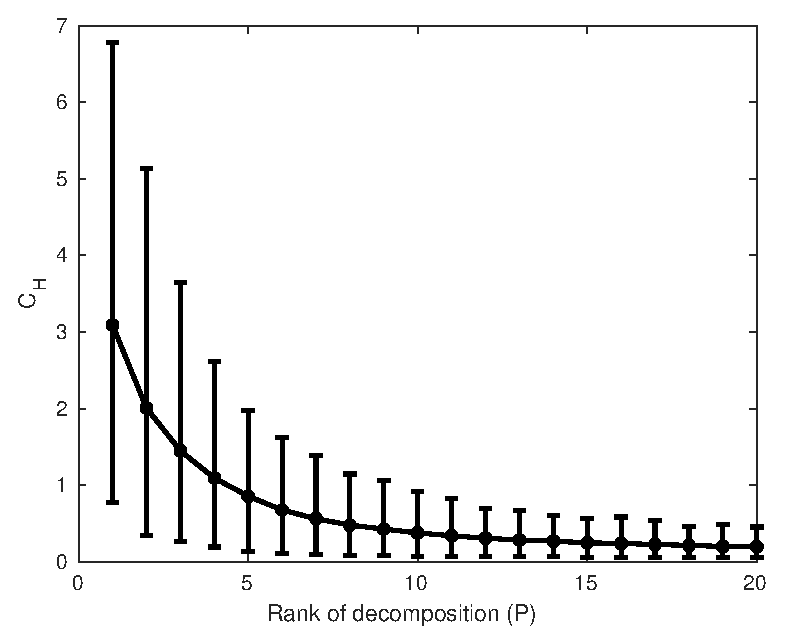
\includegraphics[width=\linewidth]{fig/RIR_NMF_approx_cost_error_plot.eps}
\caption{Effect of varying rank $P$ on the low-rank approximation for the RIR spectrogram. The deviation from the original RIR spectrogram reduces with increasing $P$. The deviation is small for $P>10$.}
\label{fig:rank_p_approximation}
\end{figure}
\iffalse
\begin{figure*}[ht]
\begin{tabular}{cccc}
\subfloat[]{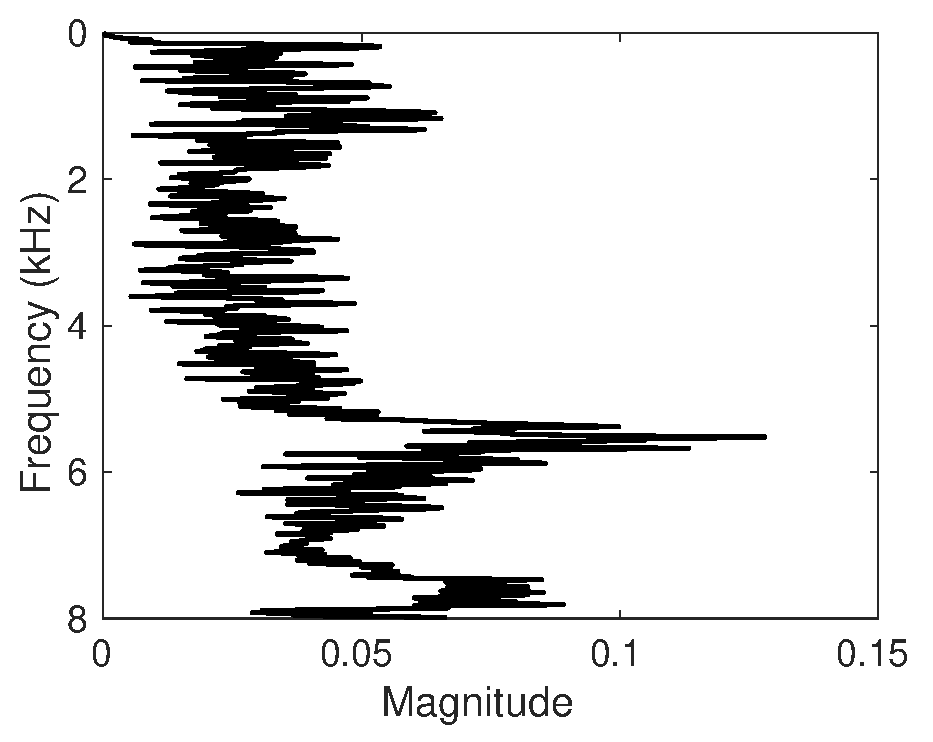
\includegraphics[width = 0.25\linewidth]{fig/RIR_env_original_RIR_cond_RIR_SimRoom3_far_AnglA_StationaryNoise_10dB.eps}} &
\subfloat[]{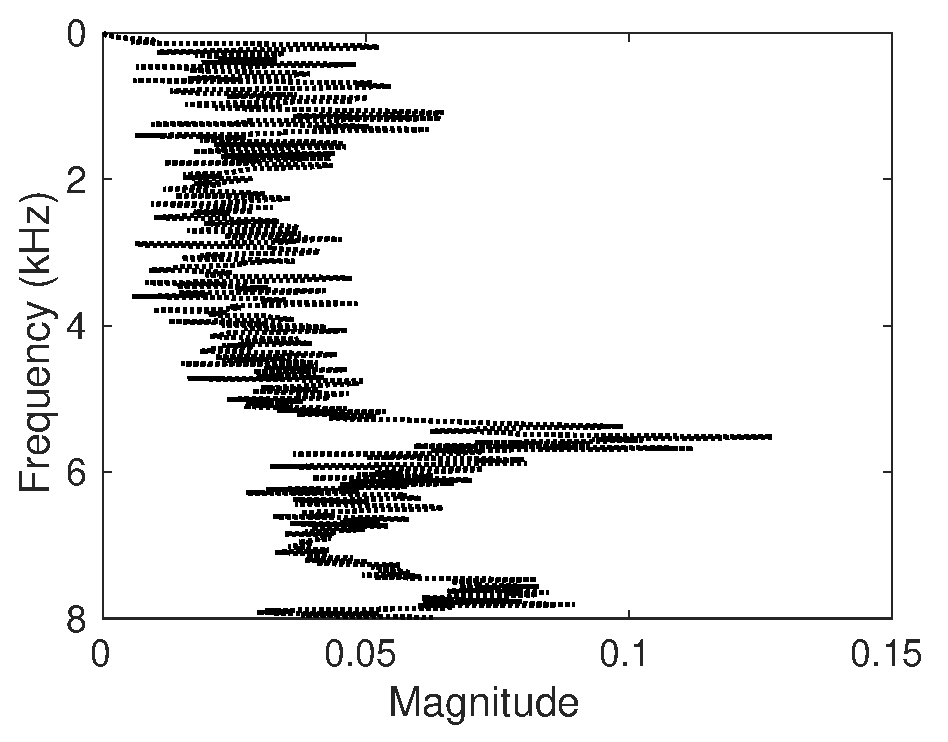
\includegraphics[width = 0.25\linewidth]{fig/RIR_env_approx_RIR_cond_RIR_SimRoom3_far_AnglA_StationaryNoise_10dB.eps}} &
\subfloat[]{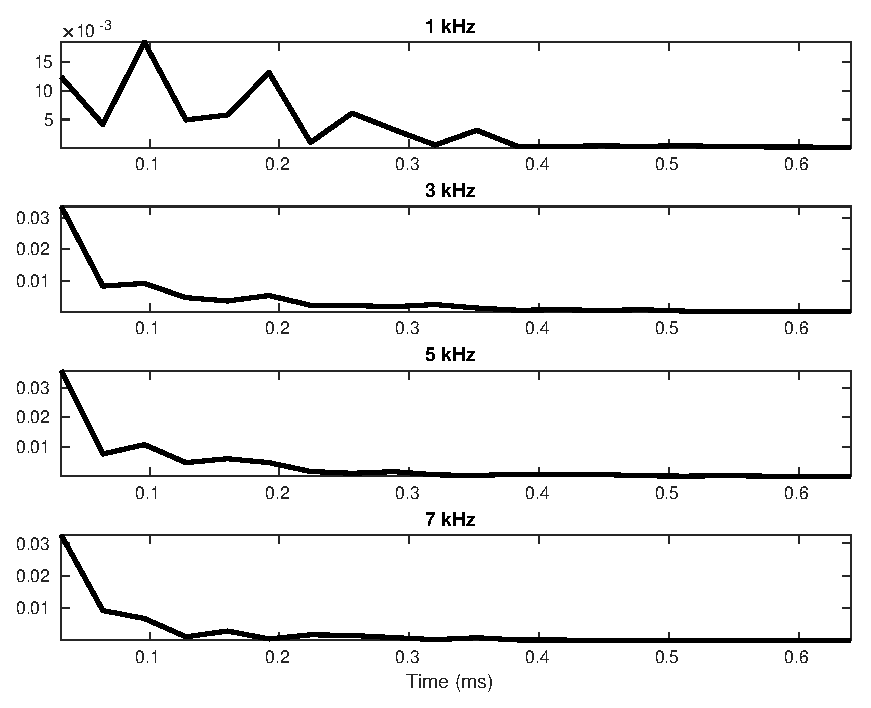
\includegraphics[width = 0.25\linewidth]{fig/RIR_tempo_original_RIR_cond_RIR_SimRoom3_far_AnglA_StationaryNoise_10dB.eps}} &
\subfloat[]{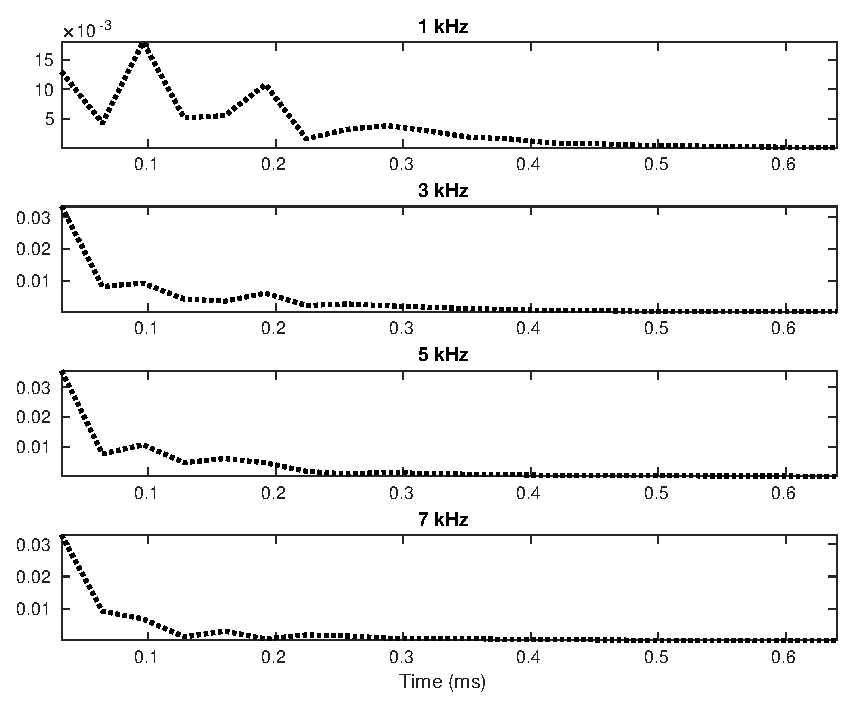
\includegraphics[width = 0.25\linewidth]{fig/RIR_tempo_approx_RIR_cond_RIR_SimRoom3_far_AnglA_StationaryNoise_10dB.eps}} \\
\end{tabular}
\caption[abc]{(a) Frequency envelope and temporal variation for different bands for the spectrogram obtained for a measured RIR from~\cite{kinoshita2016summary} having an approximate $T_{60}$ of $500$~ms and source-to-microphone distance (d) of $2$~m. (b) Frequency envelope and temporal variation obtained by a rank-$10$ NMF decomposition of the RIR. (b) is a very good approximation of (a).}
\label{fig:RIR_spectrogram}
\end{figure*}
\fi
%\iffalse
\begin{figure*}[ht]
\begin{tabular}{cc}
\subfloat[]{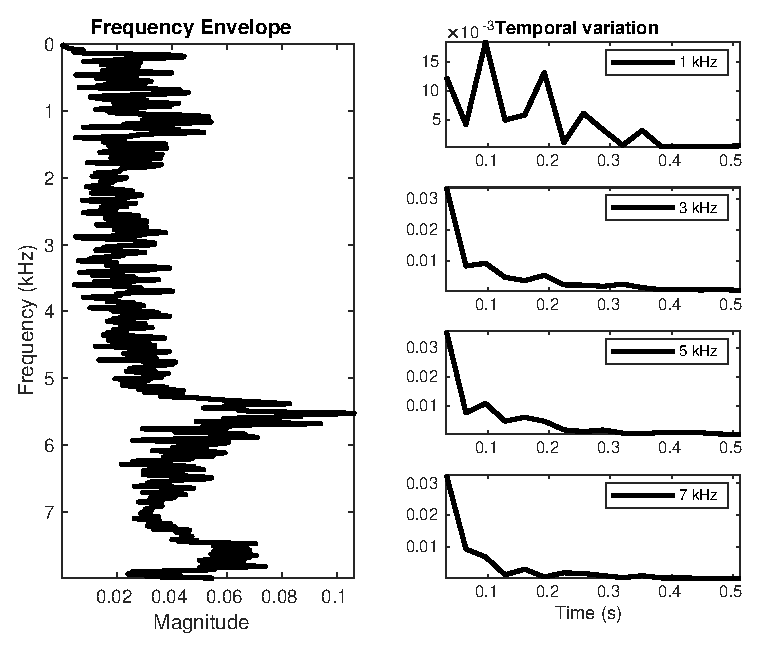
\includegraphics[width = 0.5\linewidth]{fig/RIR_NMF_far_original.eps}} &
\subfloat[]{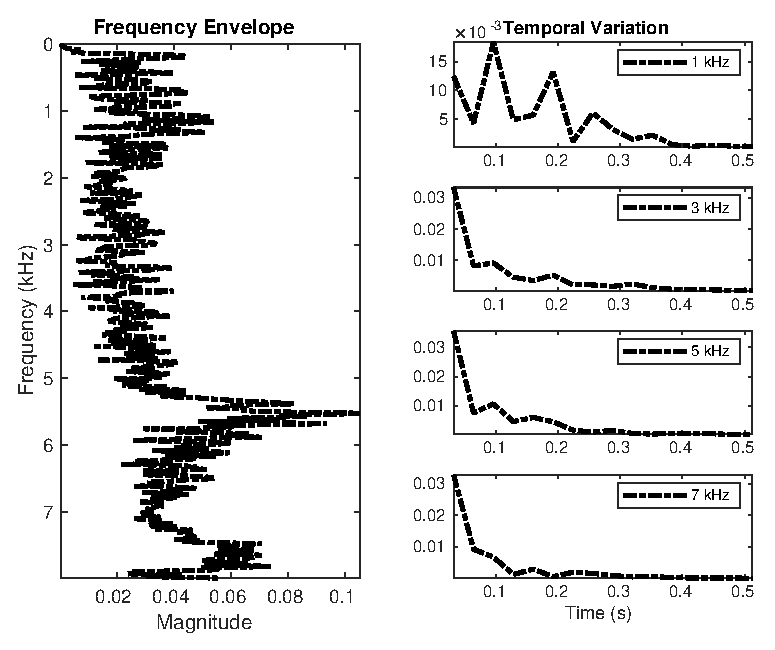
\includegraphics[width = 0.5\linewidth]{fig/RIR_NMF_far_approx.eps}}\\
\end{tabular}
\caption{(a) Frequency envelope and temporal variation obtained for a measured RIR from~\cite{kinoshita2016summary} with $T_{60}\approx 700$~ms and source-to-microphone distance $d=2$~m. (b) Frequency envelope and temporal variation obtained by a rank-$10$ NMF decomposition of the RIR. (b) is a very good approximation of (a).}
\label{fig:RIR_spectrogram}
\end{figure*}
%\fi
\iffalse
\begin{figure*}
\begin{tabular}{cc}
\subfloat[]{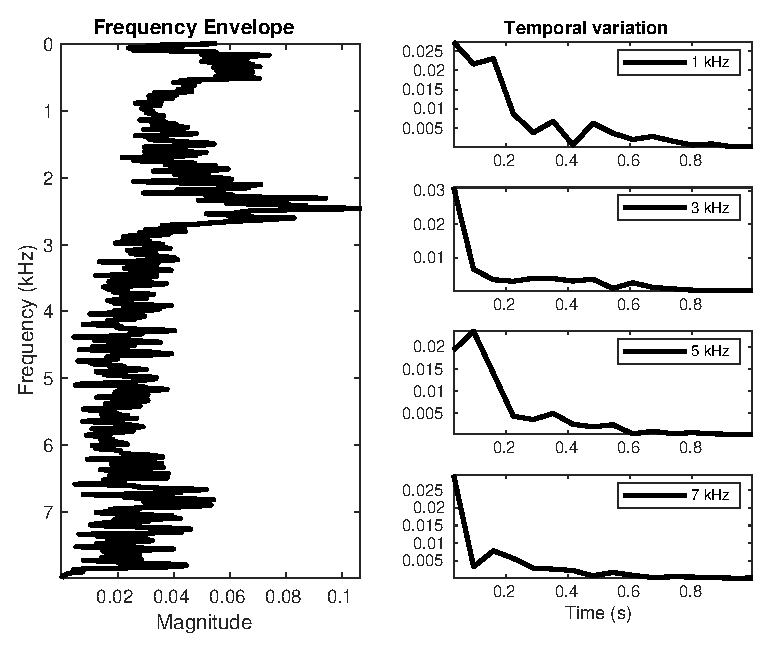
\includegraphics[width = 0.5\linewidth]{fig/RIR_NMF_near_original.eps}} &
\subfloat[]{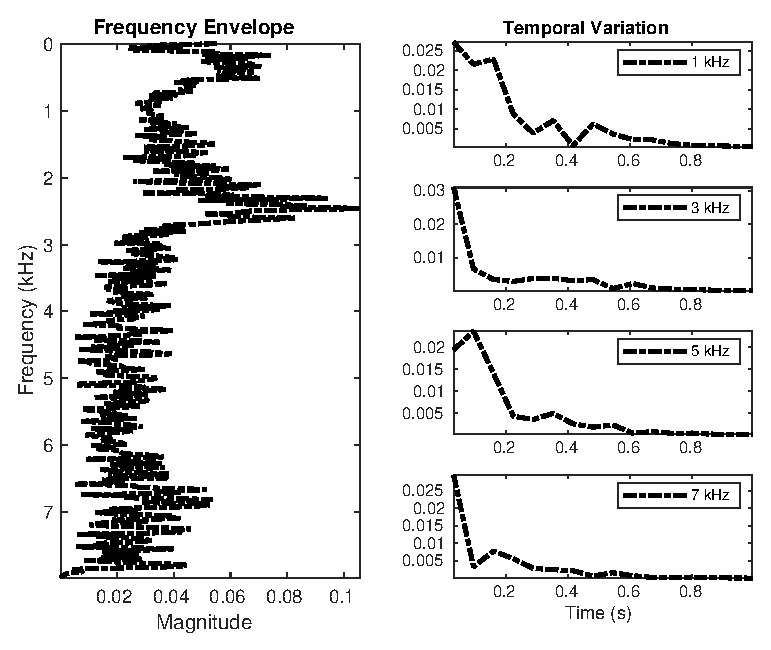
\includegraphics[width = 0.5\linewidth]{fig/RIR_NMF_near_approx.eps}}\\
\end{tabular}
\caption[abc]{(a) Frequency envelope and temporal variation for the spectrogram obtained for a measured RIR from~\cite{kinoshita2016summary} having an approximate $T_{60}$ of $500$~ms and source-to-microphone distance (d) of $0.5$~m. (b) Frequency envelope and temporal variation obtained by a rank-$10$ NMF decomposition of the RIR. (b) is a very good approximation of (a).}
%\label{fig:RIR_spectrogram}.
\label{fig:RIR_spectrogram_near}
\end{figure*}
\fi

Most of the NMF based reverberation models in literature have not considered a time-frequency model for the RIR spectrogram, though a model for speech was used. In [22], we proposed a time-frequency model for RIR spectrogram using a separability assumption. The model approximates the RIR spectrogram with a rank-$1$ NMF decomposition ($H(n, k) \approx H_1(k)H_2(n)$), where $H_1(k)$ and $H_2(n)$ represent the frequency envelope and temporal variation of RIR spectrogram, respectively. A speech enhancement algorithm was proposed using the model. It was experimentally observed that the estimated $H_1(k)$ was a good approximation to the actual frequency envelope. Further, the temporal variation $H_2(n)$ was observed to decay with $n$. The limitation of the model is it does not capture the frequency-dependent temporal variation for the RIR spectrogram. We extend the earlier model to overcome the limitation. Instead of the separability assumption used in the earlier work, we propose to use a low-rank approximation of the RIR spectrogram. The approximate RIR spectrogram is obtained using a rank-$P$ NMF decomposition. The NMF decomposition ensures that the approximated RIR spectrogram is non-negative.
%This is a requirement for using NMF based degradation model. 
The rank-$P$ NMF approximation for RIR spectrogram $\mathbf{H}$ is given by,
%Most of the NMF based reverberation models in literature have not considered a time-frequency model for the RIR spectrogram. In~\cite{mohanan201a}, we proposed a time-frequency model for RIR spectrogram using a separability assumption. The model approximates the RIR spectrogram with a rank-$1$ NMF decomposition ($H(n,k)\approx H_1(k)H_2(n)$), where $H_1(k)$ and $H_2(n)$ represent the frequency envelope and temporal variation of RIR spectrogram, respectively. A speech enhancement algorithm was proposed using the model. It was experimentally observed that the estimated $H_1(k)$ was a good approximation to the actual frequency envelope. Further, the temporal variation $H_2(n)$ was observed to decay with $n$. The limitation of the model is it cannot have frequency-dependent temporal variation for the RIR spectrogram. We extend the earlier model to overcome the limitation. Instead of the separability assumption used in the earlier work, we propose to use a low-rank approximation of the RIR spectrogram. The approximate RIR spectrogram is obtained using a rank-$P$ NMF decomposition. The NMF decomposition ensures that the approximated RIR spectrogram is non-negative. This is a requirement for using NMF based degradation model. 
%The rank-$P$ NMF approximation for RIR spectrogram $\mathbf{H}$ is represented as,
\begin{align}
\mathbf{H}&\approx\mathbf{\hat{H}}=\mathbf{H}_1\mathbf{H}_2 \nonumber \\
		  &=\underbrace{[\mathbf{H}_1^{(1)} | \mathbf{H}_1^{(2)} | ...|\mathbf{H}_1^{(P)} ]}_\textrm{$\mathbf{H}_1$} \text{ }
		  \underbrace{[\mathbf{H}_2^{(1)^T} | \mathbf{H}_2^{(2)^T} | ...|\mathbf{H}_2^{(P)^T} ]^T}_\textrm{$\mathbf{H}_2$},
\label{eq:rank-P approx}
\end{align}
where $\mathbf{H}_1^{(p)}\in \mathbb{R}_+^{K \times 1}$, and $\mathbf{H}_2^{(p)}\in \mathbb{R}_+^{1 \times L_h}$ represent the $p$-th column of $\mathbf{H}_1\in \mathbb{R}_+^{K \times P}$, and the $p$-th row of $\mathbf{H}_2\in \mathbb{R}_+^{P \times L_h}$, respectively. (\ref{eq:rank-P approx}) can also be written as,
\begin{equation}
H(k,n) \approx \sum_{p=1}^P H_1^{(p)}(k)H_2^{(p)}(n),
\label{eq:rank-P approx1}
\end{equation}
where $H_1^{(p)}(k)$ and $H_2^{(p)}(n)$ represent the $k$-th element of $\mathbf{H}^{(p)}_1$ and the $n$-th element of $\mathbf{H}^{(p)}_2$, respectively. 
The number of elements used to represent RIR spectrogram reduces from $KL_h$ to $P(K + L_h)$\footnote{The rank-$P$ used will be such that $P<L_h$ and $P << K$.}.
The elements of $\mathbf{H}_1$ and $\mathbf{H}_2$ can also be viewed in the following way. $\mathbf{H}_1^{(p)}, p \in \{1,2,...,P\}$ forms a set of $P$ frequency envelopes and $\mathbf{H}_2^{(p)}, p \in \{1,2,...,P\}$ forms the corresponding set of $P$ temporal variations for the RIR spectrogram, respectively. 

Experimentally it can be shown that the low-rank approximation $\mathbf{\hat{H}}$ is a good approximation for the original RIR spectrogram $\mathbf{H}$. RIRs available from REVERB challenge dataset~\cite{kinoshita2016summary} is used for the purpose. The RIR spectrogram is computed using a $64$~ms Hamming window with $32$~ms hop. NMF decomposition is performed on the RIR spectrogram for positive frequencies which are represented using $K=513$ and $L_h=32$.
A low-rank NMF factorization of the RIR spectrogram is obtained using the multiplicative algorithm proposed in~\cite{lee99}. We choose the generalized Kullback-Leibler (KL) divergence as the cost function. The cost function can be summarized as,
\begin{align}
&C_H = \underset{\mathbf{H}_1, \mathbf{H}_2}{\text{min}} \sum_{k,n}\text{KL} (H(k,n)|\hat{H}(k,n)), \nonumber \\
\text{where, } &\text{KL}(u|v) = u\text{log}(\dfrac{u}{v}) + v - u.
\label{eq:KLdiv}
\end{align} 
$\hat{H}(k,n)$ is the $(k,n)$-th element of the low-rank approximated RIR spectrogram $\mathbf{\hat{H}}$. $C_H$ captures the total deviation of $\hat{H}(k,n)$ from $H(k,n)$. This deviation $C_H$ depends on the rank $P$ of the decomposition. Figure~\ref{fig:rank_p_approximation} shows the mean and extreme variations in the cost function $C_H$ for different measured RIRs available in the REVERB challenge dataset~\cite{kinoshita2016summary}. It is observed that deviation $C_H$ reduces with $P$ and deviation saturates after $P = 10$ suggesting a rank-$10$ decomposition is sufficient to capture the variations in RIR. Figure~\ref{fig:RIR_spectrogram} (a) shows the frequency envelope and temporal variations obtained for a measured RIR having $T_{60}\approx 700$~ms and source-microphone distance $d=2$~m. Frequency envelope of the RIR spectrogram represents the magnitude spectrum obtained for the frame with maximum energy. Temporal variation for a particular frequency band $k=\kappa$ represents the variation of $H(\kappa,n)$ with $n$.
Figure~\ref{fig:RIR_spectrogram} (b) shows the frequency envelope and temporal variation obtained for a low-rank approximation for the RIR spectrogram. It can be observed that the approximation has captured most of the temporal and spectral variation of RIR spectrogram. A similar observation was observed for other measured RIRs.

%Figure~\ref{fig:rank_p_approximation} shows this variation for a measured RIR. It is observed that deviation reduces with $P$ and deviation saturates after $P=10$. Figure~\ref{fig:RIR_spectrogram}(b) shows the low-rank approximated spectrogram for the RIR spectrogram shown in Figure~\ref{fig:RIR_spectrogram}(a). It can be observed that the approximation has captured most of the temporal and spectral variation of RIR spectrogram.
%\begin{figure}
%\centering
%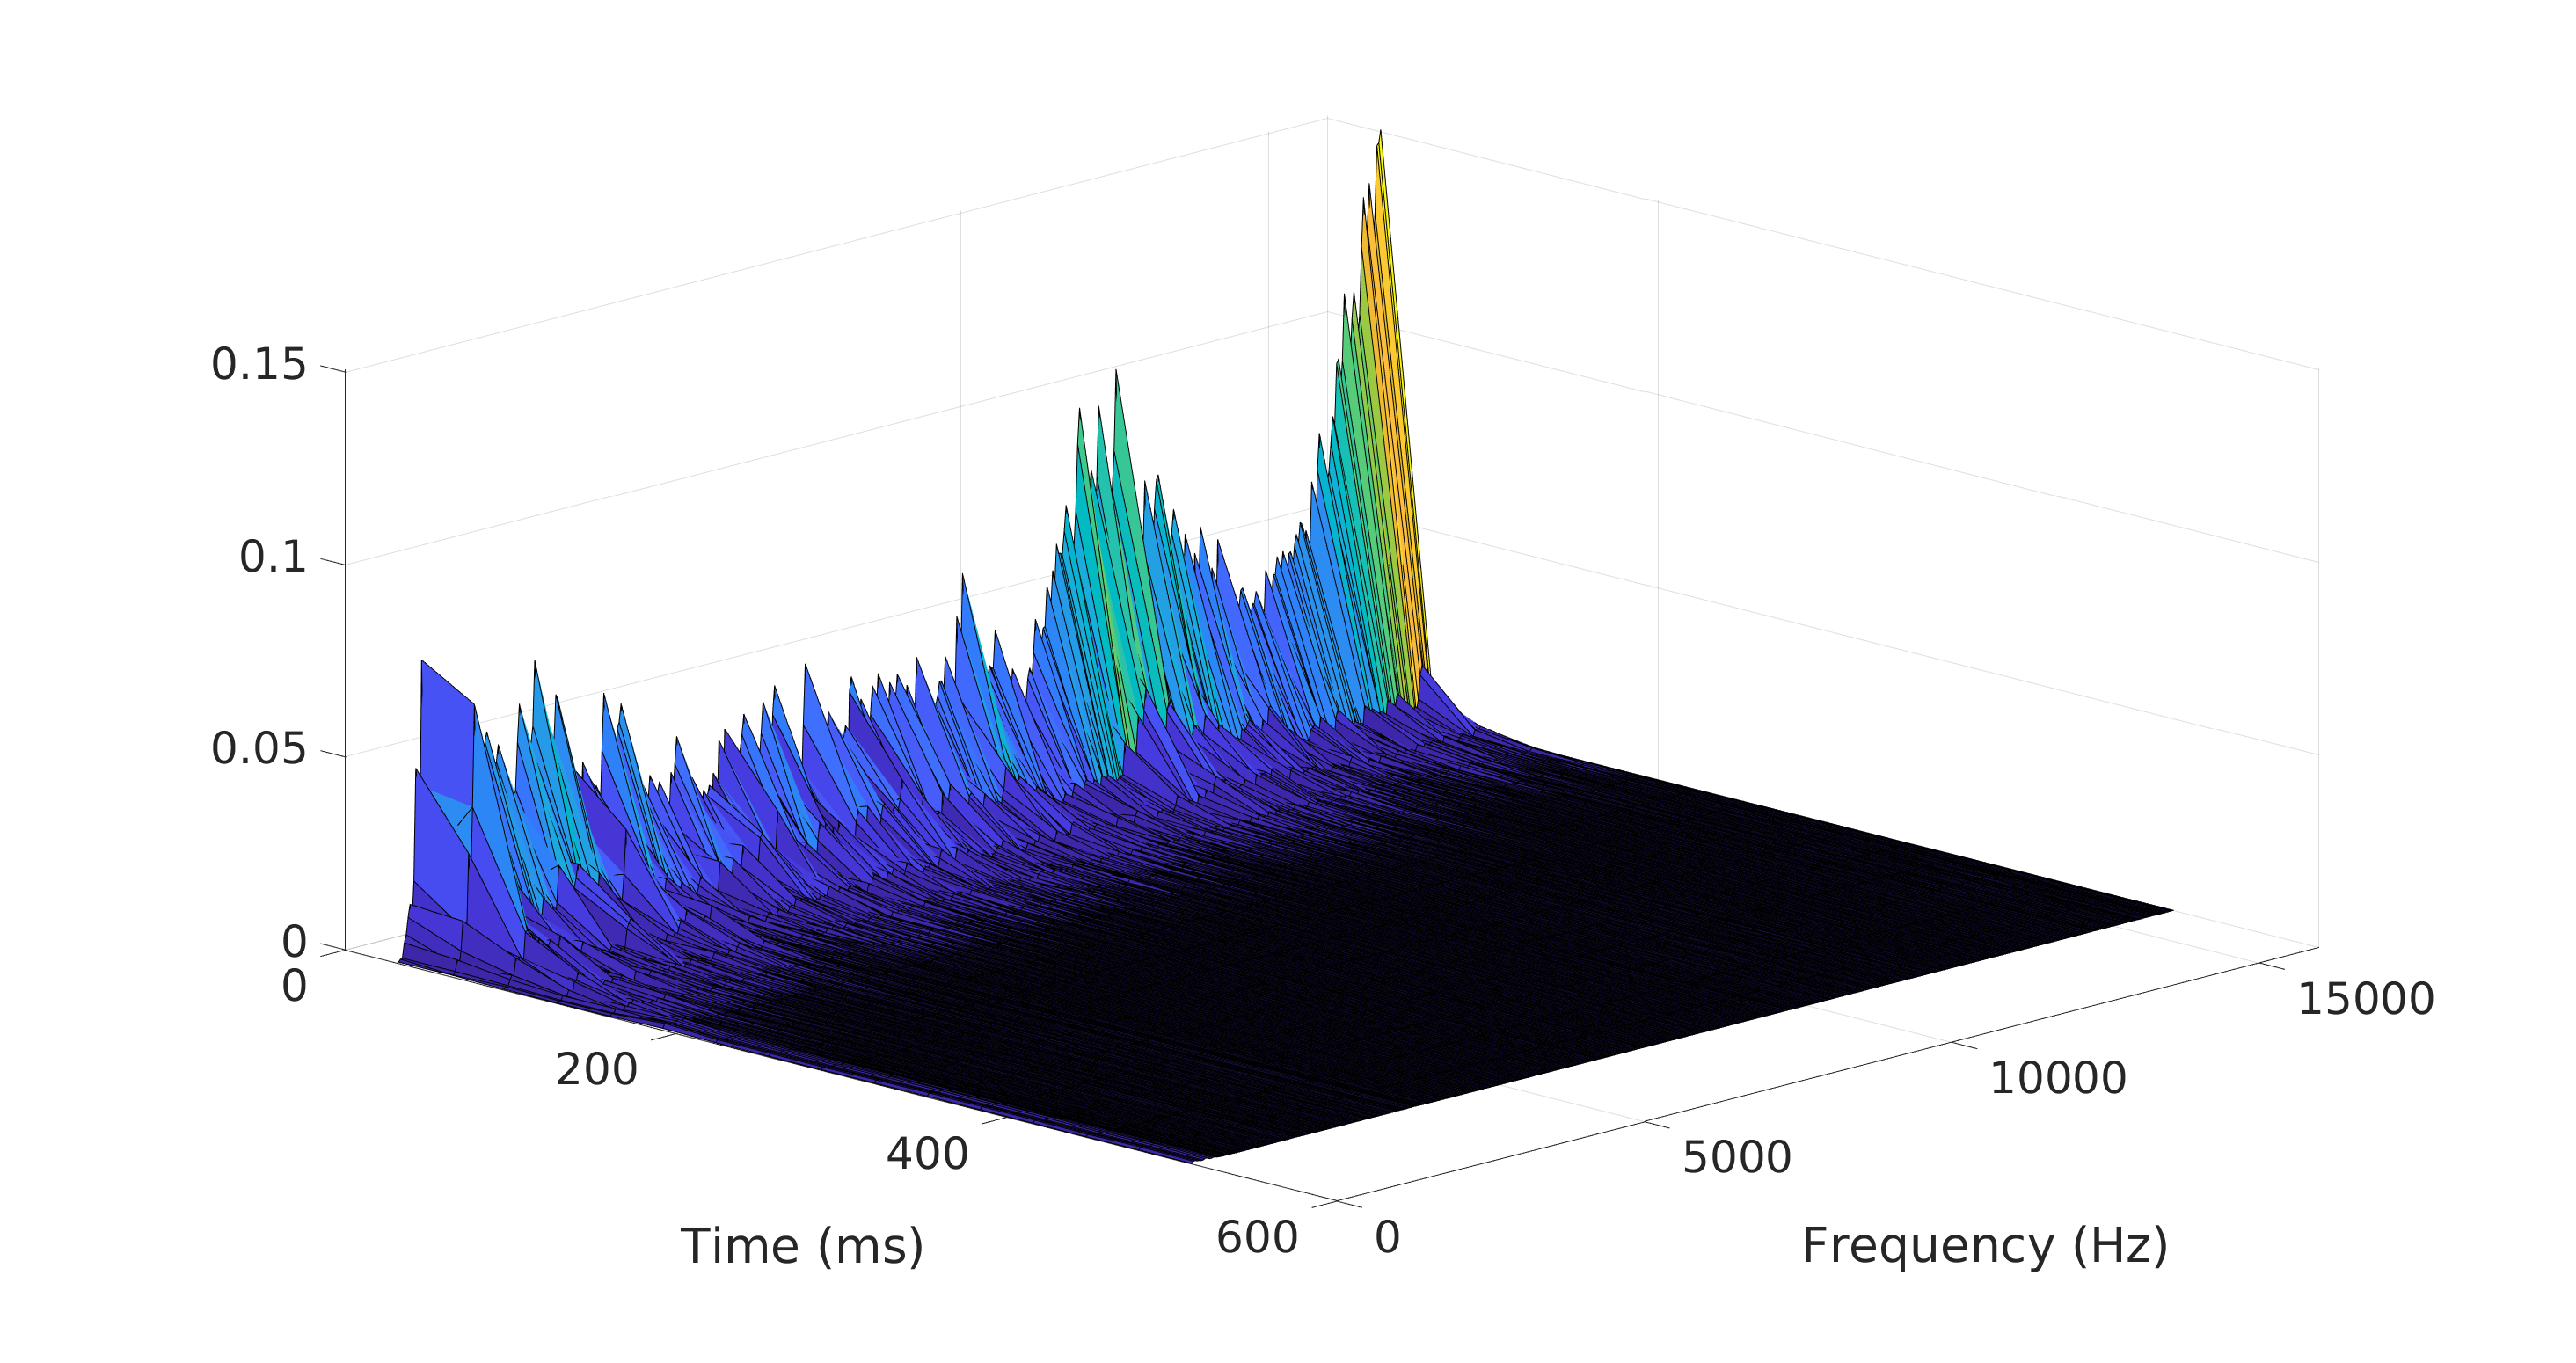
\includegraphics[width=\linewidth]{fig/RIR_approx.eps}
%\caption{The low-rank approximated RIR spectrogarm using $P=10$ for the RIR spectrogram shown in Figure~\ref{fig:RIR_spectrogram}. The original RIR spectrogram has a dimension of $513 \times 35$. The approximation is able to capture the temporal and spectral variations of the original RIR spectrogram.}
%\label{fig:RIR_approx}
%\end{figure}
%Figure~\ref{fig:RIR_spectrogram} shows the magnitude spectrogram of a measured RIR. 
%It can be observed that, the RIR spectrogram has a frequency envelope which decays with time. Also, most of the variations occur during the initial few frames after the direct path. 
\iffalse
A model for the time-frequency variation of the RIR spectrogram is discussed in \cite{wen2008blind,kuttruff2009room}. The model is based on Pollack's model for RIR. The RIR spectrogram for the model can be approximated as,
\begin{equation}
H(k,n)\approx P(k) e^{-2 \delta(k) n},
\label{eq:PollackModel}
\end{equation} 
where $P(k)$ represents the magnitude spectrum of the first frame of the RIR spectrogram ($H(k,0)$) 
%where, $P(k)$ represents the initial spectrum 
and $\delta(k)$ is related to the reverberation time ($T_{60}$) of the RIR as shown in (\ref{eq:RT60}). The $T_{60}$ (hence $\delta (k)$) changes with frequency~\cite{jeub2010we}. The variation of $T_{60}(k)$ with frequency $k$ is small for certain RIRs while for others the variation is large.  
\begin{equation}
\delta (k)= \dfrac{3\text{ln}(10)}{T_{60}(k) f_s},
\label{eq:RT60}
\end{equation}
where $f_s$ is the sampling frequency. Figure~\ref{fig:RIR_spectrogram}(a) shows the magnitude spectrogram of a measured RIR. It can be observed that the RIR spectrogram has a frequency envelope which decays with time as predicted in (\ref{eq:RT60}). The rate of decay changes with frequency as seen in the four temporal subplots in Figure~\ref{fig:RIR_spectrogram} (a) and (b). Also, most of the variations occur during the initial few frames after the direct path. The RIR spectrogram obtained based on the proposed RIR model shown in Figure~\ref{fig:RIR_spectrogram}(b) also captures these properties about RIR spectrogram. A similar behavior was observed for other RIRs and this justifies the use of the proposed RIR spectrogram model. 
\fi

\subsection{Proposed reverberation model}
This section describes the NMF model for reverberation spectrogram. Based on the low-rank approximation of the RIR spectrogram (\ref{eq:rank-P approx}), the reverb spectrogram model in (\ref{eq:deg4}) can be rewritten as,
\begin{align}
Y_R(k,n) &\approx \sum_{l=0}^{L_h-1}\sum_{p=1}^P H_1^{(p)}(k)H_2^{(p)}(l)\sum_{r=1}^R W_{\text{s}}(k,r)X_{\text{s}}(r,n-l) \nonumber \\ 
         &=\sum_{p=1}^P \sum_{r=1}^R \underbrace{W_{\text{s}}(k,r)H_1^{(p)}(k)}_\textrm{$W_R^{(p)}(k,r)$} \underbrace{ \sum_{l=0}^{L_h-1}H_2^{(p)}(l)X_{\text{s}}(r,n-l) }_\textrm{$X_R^{(p)}(r,n)$} \nonumber \\
         &= \sum_{p=1}^P \sum_{r=1}^R W_R^{(p)}(k,r)X_R^{(p)}(r,n)
\label{eq:Proposed_reverb_model}
\end{align}

Reverberation modifies the spectral and the temporal patterns of the clean speech spectrogram. In the proposed reverberation model (\ref{eq:Proposed_reverb_model}), such variations are captured by representing the reverberated speech spectrogram using NMF. The NMF model has a new set of bases $W_R^{(p)}(k,r)$ and activations $X_R^{(p)}(r,n)$. These new bases are obtained using the clean speech bases $W_{\text{s}}(k,r)$ and spectral envelopes of RIR spectrogram $H_1^{(p)}(k)$. Since the RIR spectrogram is represented using $P$ different frequency envelopes, the number of reverberated speech bases are increased by a factor of $P$. The new set of activations are obtained from clean speech activations $X_{\text{s}}(r,n)$ and temporal variation of RIR $H_2^{(p)}(n)$. The number of activations required to represent reverberated speech spectrogram also increases by a factor of $P$. This is because the RIR spectrogram contains $P$ different temporal variations. The new set of bases and activations are summarized as,
\begin{align}
W_R^{(p)}(k,r) &= W_{\text{s}}(k,r)H_1^{(p)}(k)\text{,   }p \in \{1,2,...,P\}\nonumber\\
X_R^{(p)}(r,n) &= X_{\text{s}}(r,n)*_n H_2^{(p)}(n),
\label{eq:new_model}
\end{align}
and the resulting NMF model for reverberated speech spectrogram ($\mathbf{Y}_R \approx \mathbf{W}_R\mathbf{X}_R$) is written as,
\begin{equation}
\mathbf{Y}_R \approx \underbrace{[\mathbf{W}_R^{(1)} | \mathbf{W}_R^{(2)}|...|\mathbf{W}_R^{(P)}]}_\textrm{$\mathbf{W}_R$}\ \ \underbrace{[\mathbf{X}_R^{(1)^T}|\mathbf{X}_R^{(2)^T}|...|\mathbf{X}_R^{(P)^T}]^T}_\textrm{$\mathbf{X}_R$},
\label{eq:NMF_reverb_model}
\end{equation}
%where $H_1^{(p)}(k)$ and $H_2^{(p)}(n)$ represents the $k$-th element of $\mathbf{H}^{(p)}_1$ and the $n$-th element of $\mathbf{H}^{(p)}_2$, respectively.
where $\mathbf{W}_R^{(p)} \in \mathbb{R}_+^{K \times R_s}$ and $\mathbf{X}_R^{(p)}\in \mathbb{R}_+^{R_s \times T}$ are the $p$-th block matrices of bases matrix $\mathbf{W}_R$ and activations matrix $\mathbf{X}_R$, respectively. $W_R(k,r)$ and $X_R(r,n)$ defined in (\ref{eq:new_model}) form the elements of $\mathbf{W}_R^{(p)}$ and $\mathbf{X}_R^{(p)}$, respectively. 

\subsection{Proposed joint dereverberation and denoising}
\label{sec:ProposedJointModel}
The reverberation model in~(\ref{eq:NMF_reverb_model}) can be extended to accommodate the presence of additive noise. 
The proposed approach uses an additive model to represent the degraded speech spectrogram $\mathbf{Y}$. This model is similar to the one used in~(\ref{eq:deg_model1}), where the degraded spectrogram $\mathbf{Y}$ is modeled as the sum of reverb spectrogram $\mathbf{Y}_R$ and noise spectrogram $\mathbf{Z}$. Utilizing the NMF models for noise spectrogram $\mathbf{Z}$ as in~(\ref{eq:nmf2}) and the proposed NMF model for reverberated speech spectrogram as in~(\ref{eq:NMF_reverb_model}), the degraded speech spectrogram $\mathbf{Y}$ is represented as,
\begin{align}
\mathbf{Y} & \approx \mathbf{Y}_R + \mathbf{W}_{\text{n}}\mathbf{X}_{\text{n}} = [\mathbf{W}_R| \mathbf{W}_{\text{n}}][\mathbf{X}_R^T | \mathbf{X}_{\text{n}}^T]^T. 
\label{eq:new_deg_model}
\end{align}
The bases matrix  of $\mathbf{Y}$ contains a set of bases vectors $\mathbf{W}_R$ representing reverberated speech spectrogram and another set of bases vectors $\mathbf{W}_{\text{n}}$ representing noise. Similarly, $\mathbf{X}_R$ and $\mathbf{X}_{\text{n}}$ represent the activation matrix for reverberated speech and noise spectrograms, respectively. The proposed NMF model for reverberation and noise in (\ref{eq:new_deg_model}) is easy to interpret when compared with combination of CNMF and NMF model used in (\ref{eq:deg_model2}). Further, as discussed in Section~\ref{sec:RIRconstraint} the low-rank approximation on the RIR specrogram helps in imposing better constraints on the estimated RIR spectrogram which was not possible using degradation model in (\ref{eq:deg_model2}).

\iffalse
The degraded spectrogram $\mathbf{Y}$ can be viewed as the sum of reverb spectrogram $\mathbf{Y}_R$ and noise spectrogram $\mathbf{Z}$ as in \text{CNMF2\_s}. Noise spectrogram can be approximated using a NMF model as $\mathbf{Z}\approx \mathbf{W}_n \mathbf{X}_n$, where $\mathbf{W}_n$, $\mathbf{X}_n$ represent the bases and activations of noise spectrogram, respectively. 
The degraded spectrogram $\mathbf{Y}$ can be rewritten using a NMF model as
\begin{align}
\mathbf{Y} &\approx \mathbf{Y}_R + \mathbf{Z} \approx \mathbf{Y}_R + \mathbf{W}_n\mathbf{X}_n \nonumber\\
&= [\mathbf{W}_R^{(1)} | \mathbf{W}_R^{(2)}|...|\mathbf{W}_R^{(p)}| \mathbf{W}_n][\mathbf{X}_R^{(1)^T}|\mathbf{X}_R^{(2)^T}|...|\mathbf{X}_R^{(p)^T}|\mathbf{X}_n^T]^T. 
\label{eq:new_deg_model}
\end{align}
The bases vectors of $\mathbf{Y}$ include $P$ sets of vectors to represent reverb spectrogram and a set of bases vectors to represent the noise spectrogram. Similarly, activations of degraded speech spectrogram includes $P$ sets of activations to represent reverb spectrogram and a set of activations to represent noise spectrogram. 
\fi

\section{Algorithm details}
\label{sec:cost_fn}
This section provides the algorithmic details about the proposed enhancement method. This algorithm is based on the model for reverberated and noisy speech spectrogram described in Sec~\ref{sec:ProposedJointModel}. The algorithm has a cost function associated with it that provides a measure of how well the algorithm can estimate the parameters.
An iterative approach is proposed based on the cost function to obtain an estimate for the clean speech and the RIR spectrograms.  The estimated set of parameters should ideally minimize the cost function. The first part of the section presents the proposed  enhancement algorithm. The second part of the section presents the normalization used in the algorithm.
\subsection{Joint dereverberation and denoising algorithm}
The cost function used for the proposed enhancement approach is shown in (\ref{eq:cost_enhance_rank_P}). The cost function has three terms. The  first term represents the difference between the original degraded spectrogram $\mathbf{Y}$ and the predicted degraded spectrogram $\mathbf{\tilde{Y}} = [\mathbf{W}_R | \mathbf{W}_{\text{n}}][\mathbf{X}_R^T| \mathbf{X}_{\text{n}}^T]^T$ based on generalized KL divergence. The second term is introduced to impose sparsity on estimated clean speech activation $X_{\text{s}}(r,n)$. The third term is added to impose sparsity on the noise activations $X_{\text{n}}(r,n)$. 

\begin{align}
C &= \sum_{k,n}\text{KL}(Y(k,n)|\tilde{Y}(k,n)) + \nonumber \\
& \lambda_{\text{s}} \sum_{r,n} X_{\text{s}}(r,n) + \lambda_{\text{n}} \sum_{r,n} X_{\text{n}}(r,n).
\label{eq:cost_enhance_rank_P}
\end{align}
where $\tilde{Y}(k,n)$ represents the $(k,n)$-th element of estimated degraded  spectrogram $\mathbf{\tilde{Y}}$ based on the reverberation model in (\ref{eq:new_deg_model}). The proposed cost function is similar to one used for \text{CNMF2\_s}. However, the algorithms give different solutions because $\tilde{Y}(k, n)$ in the proposed methods is estimated using a NMF model in (\ref{eq:cost_enhance_rank_P}) where as in \text{CNMF2\_s} it is obtained using a CNMF model in (\ref{eq:deg_model2}).
The multiplicative updates for clean speech and noise parameters are summarized in~(\ref{eq:update_dereverb_rank_P}).
The noise bases $W_{\text{n}}(k,r)$ and activation $X_{\text{n}}(r,n)$ are updated using standard NMF update as shown~(\ref{eq:update_enhance_rank_P}).
%The multiplicative updates obtained for the $W_s(k,r)$, $X_s(r,n)$, $H_1^{(p)}(k)$ and $H_2^{(p)}(n)$ are summarized in~(\ref{eq:update_dereverb_rank_P}).
\begin{align}
W_{\text{s}}(k,r)&\leftarrow W_{\text{s}}(k,r) \dfrac{\sum_p H_1^{(p)}(k)\sum_n \dfrac{Y(k,n)}{\tilde{Y}(k,n)}X_R^{(p)}(r,n)}{\sum_p H_1^{(p)}(k) \sum_n X_R^{(p)}(r,n)} \nonumber \\
H_1^{(p)}(k) &\leftarrow H_1^{(p)}(k)\dfrac{\sum_n\dfrac{Y(k,n)}{\tilde{Y}(k,n)}\sum_r W_{\text{s}}(k,r)X_R^{(p)}(r,n)}{\sum_n \sum_r W_{\text{s}}(k,r)X_R^{(p)}(r,n)} \nonumber \\
X_{\text{s}}(r,t) &\leftarrow X_{\text{s}}(r,t) \nonumber \\ 
         \times &\dfrac{\sum_{k,n} \dfrac{Y(k,n)}{\tilde{Y}(k,n)}  \sum_p W_R^{(p)}(k,r) H_2^{(p)}(n-t)}{\sum_{k,n}  \sum_p W_R^{(p)}(k,r) H_2^{(p)}(n-t) + \lambda_{\text{s}}} \nonumber \\
H_2^{(p)}(t) &\leftarrow H_2^{(p)}(t) \nonumber\\
\times &\dfrac{\sum_{k,n} \dfrac{Y(k,n)}{\tilde{Y}(k,n)}\sum_r W_R^{(p)}(k,r)X_{\text{s}}(r,n-t)}{\sum_{k,n} \sum_r W_R^{(p)}(k,r)X_{\text{s}}(r,n-t)}
\label{eq:update_dereverb_rank_P}
\end{align}  
%The noise bases $W_n(k,r)$ and activation $X_n(r,n)$ are updated using standard NMF update as shown~(\ref{eq:update_enhance_rank_P}).
\begin{align}
W_{\text{n}}(k,r) & \leftarrow W_{\text{n}}(k,r)\dfrac{\sum_n \dfrac{Y(k,n)}{\tilde{Y}(k,n)}X_{\text{n}}(r,n)}{\sum_n X_{\text{n}}(r,n)} \nonumber \\
X_{\text{n}}(r,n) &\leftarrow X_{\text{n}}(r,n) \dfrac{\sum_k \dfrac{Y(k,n)}{\tilde{Y}(k,n)}W_{\text{n}}(k,r)}{\sum_k W_{\text{n}}(k,r) + \lambda_{\text{n}}}
\label{eq:update_enhance_rank_P}
\end{align}
The derivations for these updates are provided in Appendix~\ref{sec:nmf_update}. The proposed NMF based joint dereverberation and denoising method will be referred to as RNMF. After the proposed NMF model converges, an estimate for the clean speech spectrogram is
obtained as $S̃(k,n)=G(k,n)Y(k,n)$. The time-varying gain function $G(k,n)$ is estimated as,
\begin{equation}
G(k,n)=\dfrac{\sum_r W_{\text{n}}(k,r)X_{\text{n}}(r,n)}{\tilde{Y}(k,n)}Y(k,n)
\label{eq:gain_function}
\end{equation}
Estimating $\tilde{S}(k,n)$ using $G(k,n)$ avoids artifacts that are introduced when $\tilde{S}(k,n)$ is estimated directly from $W_{\text{n}}(k,r)$ and $X_{\text{n}}(r,n)$~\cite{mohammadiha2016speech}. In this work, clean speech bases are assumed to be known. Depending on the way noise bases are learned there can be two different approaches - supervised approach (noise bases is also known, referred to as \text{RNMF\_s}) and semi-supervised approach (noise bases is learned from the degraded data, referred as \text{RNMF\_uk}).

\iffalse
\section{Algorithm details}
\label{sec:cost_fn}
This section provides the algorithmic details about the proposed enhancement methods. These algorithms are based on the degradation models described in Sec~\ref{sec:ProposedModel}. Iterative algorithms are proposed to obtain an estimate for the clean speech and the RIR spectrograms. Each of the algorithms has a cost function associated with it. The cost function provides a measure of how well the algorithm can estimate the parameters. The estimated set of parameters should minimize the cost function. 

\subsection{Dereverberation algorithm}
This section describes the dereverberation algorithm based on the reverberation model in (\ref{eq:Proposed_reverb_model}). The following cost function is used for the purpose. 
%The proposed approach was implemented in two stages. Such an approach will be sub-optimal as the estimate of clean activations from reverb activations is independent of estimation of other parameters in the algorithm. The two stages can be combined into a single stage approach to get better results. The stages can be combined by having additional terms in the cost function which make sure the estimated parameters are proper. The cost function used for the proposed single stage approach for reverberation using separability assumption of RIR spectrogram is shown in~(\ref{eq:cost_sep_approx_rank1}).
\begin{align}
C_R &= \sum_{k,n} \text{KL}(Y_R(k,n)|\tilde{Y}_R(k,n)) + \lambda \sum_{r,n} X_s(r,n),
\label{eq:cost_dereverb_rank_P}
\end{align}
where $\tilde{Y}_R(k,n)$ represents the estimated reverb spectrogram based on the reverberation model in (\ref{eq:Proposed_reverb_model}).  The proposed cost function is similar to one used for \text{CNMF1\_s}. However, the algorithms give different solutions because $\tilde{Y}_R(k, n)$ in the proposed methods is estimated using a NMF model in (\ref{eq:cost_dereverb_rank_P}) where as in \text{CNMF1\_s} it is obtained using a CNMF model in (\ref{eq:deg4}). The cost function has two terms. The first term represents the difference between the estimated and the actual reverberation spectrograms. The clean speech activations $X_s(k, n)$ will be spares as a few bases vectors are required to represent each frame of the clean speech spectrogram. The second term in (\ref{eq:cost_dereverb_rank_P}) is introduced to obtain a sparse solution for $X_s(k, n)$. The multiplicative updates for the cost function in (\ref{eq:cost_dereverb_rank_P}) are shown in (\ref{eq:update_dereverb_rank_P}). The detailed steps are provided in Appendix~\ref{sec:update_dereverb_1},~\ref{sec:update_dereverb_2}.

\begin{align}
W_s(k,r)&\leftarrow W_s(k,r) \dfrac{\sum_p H_1^{(p)}(k)\sum_n \dfrac{Y_R(k,n)}{\tilde{Y}_R(k,n)}X_R^{(p)}(r,n)}{\sum_p H_1^{(p)}(k) \sum_n X_R^{(p)}(r,n)} \nonumber \\
H_1^{(p)}(k) &\leftarrow H_1^{(p)}(k)\dfrac{\sum_n\dfrac{Y_R(k,n)}{\tilde{Y}_R(k,n)}\sum_r W_s(k,r)X_R^{(p)}(r,n)}{\sum_n \sum_r W_s(k,r)X_R^{(p)}(r,n)} \nonumber \\
X_s(r,t) &\leftarrow X_s(r,t) \nonumber \\ 
         \times &\dfrac{\sum_{k,n} \dfrac{Y_R(k,n)}{\tilde{Y}_R(k,n)}  \sum_p W_R^{(p)}(k,r) H_2^{(p)}(n-t)}{\sum_{k,n}  \sum_p W_R^{(p)}(k,r) H_2^{(p)}(n-t) + \lambda} \nonumber \\
H_2^{(p)}(t) &\leftarrow H_2^{(p)}(t) \nonumber\\
\times &\dfrac{\sum_{k,n} \dfrac{Y_R(k,n)}{\tilde{Y}_R(k,n)}\sum_r W_R^{(p)}(k,r)X_s(r,n-t)}{\sum_{k,n} \sum_r W_R^{(p)}(k,r)X_s(r,n-t)}
\label{eq:update_dereverb_rank_P}
\end{align}
%The proposed dereverberation method is refered to as $RNMF\-P$.
%The first term in cost function minimizes the reconstruction error. The second and third terms acts as regularizes in estimating proper estimates of the clean speech bases and activations, respectively. The parameters $\alpha$ and $\beta$ represents the relative weights given for estimated of clean speech bases and activation. These parameters are fixed by cross-validation. This method is referred to as R-NMF-$1$. Multiplicative updates can be used to simultaneously estimate the parameters. The estimated update rules are listed in~(\ref{eq:mult_update_sep_approx_rank1}). 

\subsection{Joint dereverberation and denoising}
The proposed dereverberation approach can be extended to jointly handle reverberation and noise. 
%The approach is a semi-supervised approach, i.e., the noise bases are assumed to be available. 
The cost function used for the proposed enhancement approach is shown in (\ref{eq:cost_enhance_rank_P}). The cost function has a form similar to the one used in~(\ref{eq:cost_dereverb_rank_P}). The cost function has three terms. The  first term represents the difference between the original degraded spectrogram $\mathbf{Y}$ and the predicted degraded spectrogram $\mathbf{\tilde{Y}} = [\mathbf{W}_R | \mathbf{W}_n][\mathbf{X}_R^T| \mathbf{X}_n^T]^T$ based on generalized KL divergence. The second term is introduced to impose sparsity on estimated clean speech activation $X_s(r,n)$. The third term is added to impose sparsity on the noise activations $X_n(r,n)$. 

\begin{align}
C &= \sum_{k,n}\text{KL}(Y(k,n)|\tilde{Y}(k,n)) + \nonumber \\
& \lambda_s \sum_{r,n} X_s(r,n) + \lambda_n \sum_{r,n} X_n(r,n).
\label{eq:cost_enhance_rank_P}
\end{align}
The multiplicative updates obtained for the $W_s(k,r)$, $X_s(r,n)$, $H_1^{(p)}(k)$ and $H_2^{(p)}(n)$ based on the cost function (\ref{eq:cost_enhance_rank_P}) are related to updates obtained in~(\ref{eq:update_dereverb_rank_P}). In the new updates, $Y_R(k.n)$, $\tilde{Y}_R(k,n)$ and $\lambda$ used in~(\ref{eq:update_dereverb_rank_P}) are replaced by $Y(k,n)$, $\tilde{Y}(k,n)$ and $\lambda_s$, respectively. Additionally, the noise bases $W_n(k,r)$ and activation $X_n(r,n)$ are updated using standard NMF update as shown. 
\begin{align}
W_n(k,r) & \leftarrow W_n(k,r)\dfrac{\sum_n \dfrac{Y(k,n)}{\tilde{Y}(k,n)}X_n(r,n)}{\sum_nX_n(r,n)} \nonumber \\
X_n(r,n) &\leftarrow X_n(r,n) \dfrac{\sum_k \dfrac{Y(k,n)}{\tilde{Y}(k,n)}W_n(k,r)}{\sum_k W_n(k,r) + \lambda_n}
\label{eq:update_enhance_rank_P}
\end{align}
The detailed steps are shown in Appendix~\ref{sec:update_noise}. The proposed
NMF based joint dereverberation and denoising method will be referred to as RNMF. After the proposed NMF model converges, an estimate for the clean speech spectrogram is
obtained as $S̃(k,n)=G(k,n)Y(k,n)$. The time-varying gain function $G(k,n)$ is estimated as,
\begin{equation}
G(k,n)=\dfrac{\sum_r W_s(k,r)X_s(r,n)}{\tilde{Y}(k,n)}Y(k,n)
\label{eq:gain_function}
\end{equation}
%The detailed steps are shown in Appendix~\ref{sec:update_noise}.
%The proposed NMF based joint dereverberation and denoising method will be referred to as RNMF. In this experiments, clean speech bases are assumed to be known. Depending on the way noise bases are learned there can be two different approaches - supervised approach (noise bases is also known, referred to as \text{RNMF\_s}) and semi-supervised approach (noise bases is learned from the degraded data, referred as \text{RNMF\_uk}). An estimate for the clean speech spectrogram is obtained as $\tilde{S}(k,n)=G(k,n)Y(k,n)$. The time-varying gain function $G(k,n)$ is estimated as,
Estimating $\tilde{S}(k,n)$ using $G(k,n)$ avoids artifacts that are introduced when $\tilde{S}(k,n)$ is estimated directly from $W_s(k,r)$ and $X_s(r,n)$~\cite{mohammadiha2016speech}. In this work, clean speech bases are assumed to be known. Depending on the way noise bases are learned there can be two different approaches - supervised approach (noise bases is also known, referred to as \text{RNMF\_s}) and semi-supervised approach (noise bases is learned from the degraded data, referred as \text{RNMF\_uk}).
%Estimating $\tilde{S}(k,n)$ using $G(k,n)$ avoids the occurrence of artifacts which are introduced when $\tilde{S}(k,n)$ is estimated directly from $W_s(k,r)$ and $X_s(r,n)$~\cite{mohammadiha2016speech}.
\fi
\subsection{Normalization}
\label{sec:normaization}
The normalization of the estimated parameters is critical for NMF based enhancement methods. It removes the inherent scaling ambiguity present in the cost functions. Each of the clean speech and noise bases vectors learned are normalized to have unit $\ell_2$-norm. 
In~\cite{mohammadiha2016speech}, the estimated $\mathbf{H}$ is normalized to have all-one vector for first column of $\mathbf{H}$. The estimated $\mathbf{H}_1$ and $\mathbf{H}_2$ are normalized in the same manner. The columns of $\mathbf{H}_1$ are normalized to sum to one. Each columns of $\mathbf{H}_2$ are divided element-wise with the first column of $\mathbf{H}_2$. Further, in \text{CNMF1\_s}~\cite{mohammadiha2016speech} and \text{CNMF2\_s}~\cite{baby2015coupled} the estimated RIR spectrogram is truncated so that $H(k,n) \leq H(k,n-1)$. Such a constraint on the RIR spectrogram is true only for the latter frames. Some of the initial frames (especially in far cases) can have $H(k,n) > H(k,n-1)$. So, in the proposed method, the truncation on estimated $H_2^{(p)}(n)$ is applied for $n\geq10$.
The normalization used for RNMF can be summarized as
\begin{align}
\mathbf{W}_x^{(t)} &\leftarrow \dfrac{\mathbf{W}_x^{(t)}}{|| \mathbf{W}_x^{(t)}||_2}, \text{     } x\in\{\text{s, n}\}\nonumber\\
H_1^{(p)}(k) &\leftarrow \dfrac{H_1^{(p)}(k)}{ \sum_p H^{(p)}_1(k)}, \text{   }p\in \{1,2,...,P\},\nonumber\\
H_2^{(p)}(n) &\leftarrow \dfrac{H_2^{(p)}(n)}{H^{(p)}_2(1)}, \nonumber\\
H_2^{(p)}(n) &\leftarrow \text{min}(H_2^{(p)}(n), H_2^{(p)}(n-1)), \text{ } n\geq10,
\label{eq:normalizations}
\end{align}    
where $\mathbf{W}_x^{(t)}$ represents the $t$-th column of the bases matrix $\mathbf{W}_x$.

\section{Experimental setup}
This section presents the experimental setup used for the evaluation of the proposed algorithm. The algorithm is compared with CNMF0~\cite{kameoka2009robust}, \text{CNMF1\_s}~\cite{mohammadiha2016speech} and \text{CNMF2\_s}~\cite{baby2015coupled}. The performance of the algorithms is compared based on speech enhancement results. Perceptual evaluation of speech quality (PESQ)~\cite{recommendation2001perceptual}, cepstral distance (CD)~\cite{hu2008evaluation}, speech-to-reverberation modulation energy ratio  (SRMR)~\cite{falk2010non}, and Mel-frequency cepstral coefficient distance (MFCCD)~\cite{yoshioka2009integrated} are the objective measures used for evaluation. PESQ is a measure of perceptual similarity of an enhanced speech to the target speech.
CD measure correlates well with speech distortion, overall quality, and dereverberation performance. Improvements in MFCCD is related to the ASR improvements of dereverberation algorithms. SRMR gives a measure of dereverberation performance.
Table~\ref{tab:Methods} summarizes the various enhancement methods considered in this work. The methods are distinguished based on the use of NMF models for clean speech and noise spectrograms and the way noise bases $\mathbf{W}_n$ are obtained.
\begin{table}[h]
\centering
\caption{A summary of methods compared in this work. Proposed approaches are represented in bold.} 
\begin{tabular}{|l|c|c|c|c|}
\hline
\multicolumn{1}{|c|}{\multirow{2}{*}{\textbf{Method}}} & \multicolumn{2}{c|}{\textbf{Clean speech model}} & \multicolumn{2}{c|}{\textbf{Noise model}} \\ \cline{2-5} 
\multicolumn{1}{|c|}{}                                 & \textbf{Used}       & \textbf{Pre-learned bases}       & \textbf{Used}    & \textbf{Pre-learned bases}   \\ \hline
CNMF0    & $\times$     & $\times$    & $\times$     & $\times$      \\ \hline
\text{CNMF1\_s} & $\checkmark$  & $\checkmark$ & $\times$     & $\times$      \\ \hline
\text{CNMF2\_s} & $\checkmark$  & $\checkmark$ & $\checkmark$  & $\checkmark$   \\ \hline
\textbf{RNMF\_uk} & $\checkmark$  & $\checkmark$    & $\checkmark$  & $\times$   \\ \hline
\textbf{RNFM\_s}  & $\checkmark$  & $\checkmark$ & $\checkmark$  & $\checkmark$   \\ \hline
\end{tabular}
\label{tab:Methods}
\end{table}
%Some initial results on ASR performance is also discussed.
\label{sec:experiment}
\subsection{Dataset}
The degraded data was generated using clean recordings available in the TIMIT dataset~\cite{garofolo1993timit}. The set contained $16$ different utterances selected from $16$ different speakers. This set was used to analyze the performance when using speaker-dependent (SD) and speaker-independent (SI) clean speech bases vectors.

Reverberation was simulated by convolving the clean utterances with four different measured RIRs available from REVERB challenge database~\cite{kinoshita2016summary}. The RIR $T_{60}$, source-microphone distance ($d$) and direct-to-reverberation ratios
($D_{50}$) used for the measurements are summarized in in Table~\ref{tab:RIR_cond}. $D_{50}$ gives a measure of extent of spectral coloration and reverberation tail. RIRs with $d=0.5$~m have higher $D_{50}$. Effects of spectral coloration will be dominant for these RIRs. Since the proposed approach uses a model for RIR frequency envelope, the enhancement results will be better for such RIRs.
The reverberated data is also added with stationary noise (caused mainly by air conditioning systems in a room) available from REVERB challenge~\cite{kinoshita2016summary}. The reverberated and noisy speech is obtained by adding a random segment of the noise at $10$~dB and $20$~dB signal-to-noise ratios (SNRs) to the reverberated speech. 
The performance of the algorithms is compared across eight different degradation conditions (four reverberation and two SNR conditions).  

\begin{table}[ht]
\centering
\caption{The approximate $T_{60}$, source-microphone distance ($d$) and $D_{50}$ of the measured RIRs.}
\begin{tabular}{|l|c|c|c|}
\hline
\textbf{RIR} & \textbf{$T_{60}$ (ms)} & d\textbf{ (m)} & $D_{50}$\textbf{ (\%)} \\ \hline
R2\_near     & 600                    & 0.5            & 95                \\ \hline
R2\_far      & 600                    & 2.0            & 79                \\ \hline
R3\_near     & 700                    & 0.5            & 97                \\ \hline
R3\_far      & 700                    & 2.0            & 81                \\ \hline
\end{tabular}
\label{tab:RIR_cond}
\end{table}

\subsection{Spectrogram parameters and bases creation}
The enhancements are performed on the positive half of the magnitude spectrogram of the degraded speech. 
%The spectrogram parameters are fixed as in~\cite{mohammadiha2016speech}. 
This magnitude spectrogram is obtained by performing a STFT on the degraded speech utterance using a $1024$ point ($64$~ms) Hamming window with a $512$ point ($32$~ms) hop. To include the temporal context in the speech spectrograms, frame stacking of six frames was done as suggested in~\cite{mohammadiha2016speech}. Frame stacking is done by appending the frame-shifted versions of the original spectrogram to itself. The frame stacking can be summarized as
%(\ref{eq:Frame_stacking}). 
\begin{align}
\mathbf{Y}^{stack} = [\mathbf{Y}^T| \mathbf{Y}^{\leftarrow (1)^T} | \dots |\mathbf{Y}^{\leftarrow (N-1)^T}]^T.
\label{eq:Frame_stacking}
\end{align}
\iffalse
\begin{align}
\mathbf{Y}^{stack} = \begin{bmatrix}
\mathbf{Y} \\
\mathbf{Y}^{\leftarrow (1)} \\
\vdots \\
\mathbf{Y}^{\leftarrow (N-1)}
\end{bmatrix}.
\label{eq:Frame_stacking}
\end{align}
\fi
The resulting frame has a dimension of $NK \times T$, where $N$ and $\mathbf{Y}^{stack} \in \mathbb{R}_+^{NK \times T}$ represent the number of frames stacked and the stacked degraded spectrogram, respectively. $\mathbf{Y}^{\leftarrow (N-1)}$ used in (\ref{eq:Frame_stacking}) can be obtained from $\mathbf{Y}=[\mathbf{Y}_{(1)}, \mathbf{Y}_{(2)}, ...,\mathbf{Y}_{(T)}]$ as shown in (\ref{eq:Frame_shifting}).
\begin{align}
\mathbf{Y}^{\leftarrow (N)} &= \begin{bmatrix}
\underbrace{\mathbf{Y}_{(N+1)} \text{ ... } \mathbf{Y}_{(T)}}_{T-N} & \underbrace{\mathbf{0}\text{...} \mathbf{0}}_{N}
\end{bmatrix},
\label{eq:Frame_shifting}
\end{align}
\iffalse
\begin{align}
\mathbf{Y}&=[\mathbf{Y}_{(1)}, \mathbf{Y}_{(2)}, ...,\mathbf{Y}_{(T)}] \nonumber \\
\mathbf{Y}^{\leftarrow (N)} &= \begin{bmatrix}
\underbrace{\mathbf{Y}_{(N+1)} \text{ ... } \mathbf{Y}_{(T)}}_{T-N} & \underbrace{\mathbf{0}\text{...} \mathbf{0}}_{N}
\end{bmatrix},
\label{eq:Frame_shifting}
\end{align}
\fi
where, $\mathbf{Y}_{(t)}$ and $\mathbf{0}$ represent the $t$-th column of $\mathbf{Y}$ and a zero vector of length $NK$, respectively.

A set of $100$ SD bases vectors are learned for each speaker. The bases vectors are learned from nine utterances spoken by the same speaker
%. These utterances exclude the one used for evaluation. Bases vectors are learned 
by performing a NMF decomposition on the magnitude spectrogram of these utterances. The SI bases vectors are learned from the magnitude spectrogram constructed using a subset of the train set of TIMIT. $250$ utterances spoken by different speakers are randomly selected from the train set. A set of $400$ clean speech bases vectors are learned from the magnitude spectrogram of the selected utterances. 

The noise recordings available are divided equally into train and test set. The train set is used to obtain the noise bases and test set is used to simulate degraded utterances. A NMF decomposition is performed on the magnitude spectrogram of the train set to obtain a set of noise bases vectors. A set of $100$ noise bases vectors are learned for the noise condition. This forms the noise bases matrix $\mathbf{W}_n$ used in supervised enhancement methods \text{CNMF2\_s} and \text{RNMF\_s}. Supervised enhancement methods that use SD bases will use $100$ noise bases and $100$ SD clean speech bases, whereas the SI case uses $100$ noise bases and $400$ SI clean speech bases.

\subsection{Choice of initialization and hyper-parameters}
For the proposed method RNMF, the hyper-parameters are initialized in the following manner.  Initial estimates for clean speech spectrogram $\mathbf{S}$ and RIR spectrogram $\mathbf{H}$ are obtained using (\ref{eq:deg2}). Clean speech activations $\mathbf{X}_{\text{s}}$ is obtained by performing a NMF decomposition on the estimated $\mathbf{S}$. A NMF decomposition on RIR spectrogram $\mathbf{H}$ is used to get an initial estimate for $\mathbf{H}_1$ and $\mathbf{H}_2$. The reverberated speech bases $\mathbf{W}_R$ and activations $\mathbf{X}_R$ are initialized using (\ref{eq:new_model}). For the supervised method \text{RNMF\_s}, noise activations $\mathbf{X}_{\text{n}}$ is initialized with random positive numbers. For the semi-supervised approach \text{RNMF\_uk}, an initial estimate of noise bases $\mathbf{W}_{\text{n}}$ and activations $\mathbf{X}_{\text{n}}$ are obtained using multiplicative updates shown in~(\ref{eq:update_enhance_rank_P}).

The algorithms compared in this work have cost function with terms to promote sparsity. For the reference methods CNMF0 and \text{CNMF1\_s}, the sparsity terms are fixed as in the original paper. For the reference method \text{CNMF2\_s}, sparsity terms are set as $\lambda_{\text{s}} = \lambda_{\text{n}} = 10^{-8}$. It was observed that \text{CNMF2\_s} gives better results with these regularizers. The reason for such an observation was that \text{CNMF2\_s} in~\cite{baby2015coupled} was proposed to work with exemplar bases. A large number of bases vectors are required when exemplar bases are used. However, in this work learned bases are used. So, less number of bases vectors are used. Hence, the activations were less sparse. Sparsity terms used for the proposed methods differ depending on the type of clean speech and noise bases used. \text{RNMF\_s} uses $\lambda_{\text{s}}=0.1, \lambda_{\text{n}}=10^{-8}$. Sparsity terms for \text{RNMF\_uk} is fixed as $\lambda_{\text{s}}=0.1, \lambda_{\text{n}}=10$. RIR spectrograms are represented using $L_h=20$.
The rank of the RIR spectrogram decomposition was fixed as $P = 10$ based on observations made in Figure~\ref{fig:rank_p_approximation}. 
All the enhancement algorithms run for $100$ NMF iterations. The phase spectrogram of the degraded utterance along with the enhanced magnitude spectrogram was used to obtain the corresponding enhanced time-domain signal.

\begin{figure}[h]
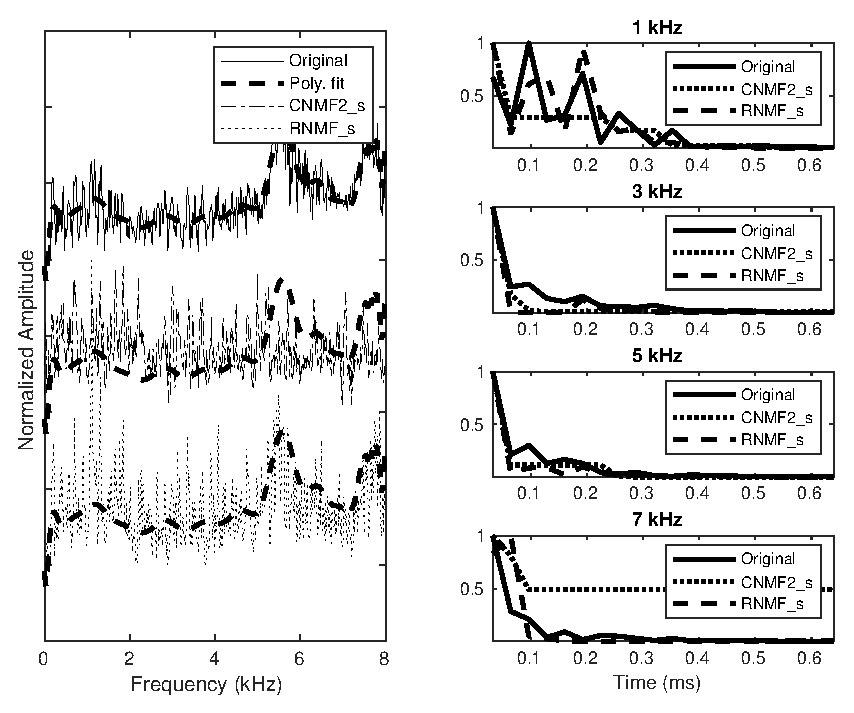
\includegraphics[width = \linewidth]{fig/RIR_comparison_SpkId_12_RIR_cond_RIR_SimRoom3_far_AnglA_StationaryNoise_10dB.eps}
\caption{Comparison of the estimated frequency envelope and temporal variation for different enhancement methods when the RIR used is \text{R3\_far}. \text{RNMF\_s} gives better RIR estimate when compared to \text{CNMF2\_s}.}
\label{fig:RIR_spectrogram_comparison}
\end{figure}
\iffalse
\begin{figure*}[h]
\begin{tabular}{cc}
\subfloat[]{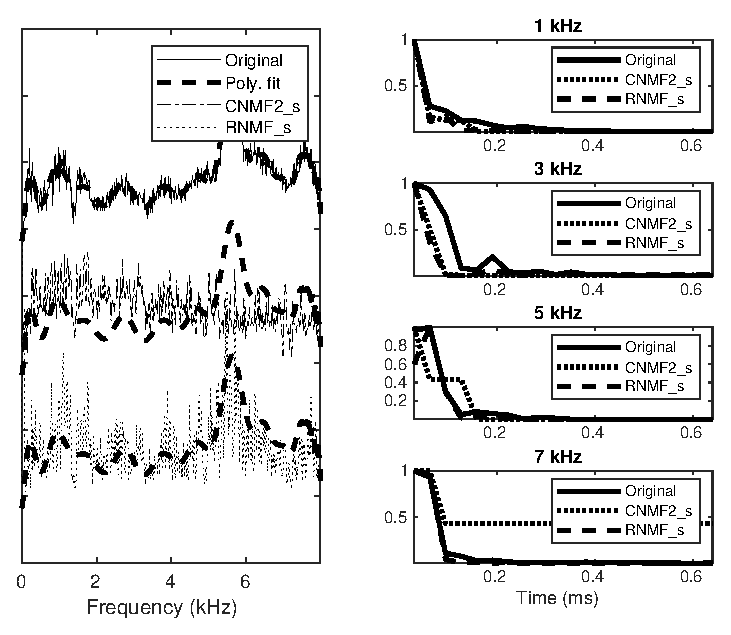
\includegraphics[width = 0.5\linewidth]{fig/RIR_comparison_SpkId_12_RIR_cond_RIR_SimRoom3_near_AnglA_StationaryNoise_10dB.eps}} &
\subfloat[]{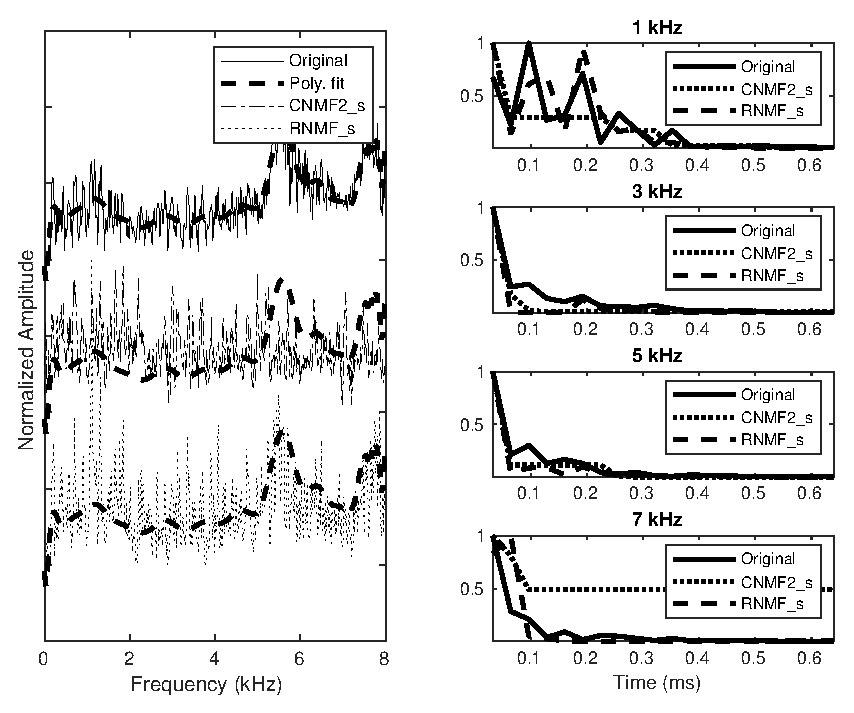
\includegraphics[width = 0.5\linewidth]{fig/RIR_comparison_SpkId_12_RIR_cond_RIR_SimRoom3_far_AnglA_StationaryNoise_10dB.eps}}\\
\end{tabular}
\caption[abc]{Frequency envelope and temporal variation for the RIR spectrogram obtained for differnt enhancement methods when (a) RIR \text{R3\_near} is used, (b) RIR \text{R3\_far} is used. RNMF methods gives better RIR estimate when compared to \text{CNMF2\_s}.}
%\label{fig:RIR_spectrogram}.
\label{fig:RIR_spectrogram_comparison}
\end{figure*}
\fi
\subsection{Results}
This section presents the performance of various enhancement methods. The proposed enhancement algorithms are compared with reference methods separately when using SD
and SI clean bases.

The performance of the various algorithms was compared for speech enhancement task. The performance was evaluated based on the relative improvements on the enhancement measures, such as PESQ~\cite{recommendation2001perceptual}, CD~\cite{hu2008evaluation},  SRMR~\cite{falk2010non}, and MFCCD~\cite{yoshioka2009integrated}. Enhanced speech is expected to have a higher PESQ and SRMR value as compared to the corresponding degraded speech. The CD and MFCCD values decrease with improving speech quality. The relative improvements in enhancement measures are represented as $\Delta$ PESQ, $\Delta$ CD, $\Delta$ SRMR, and  $\Delta$ MFCCD respectively.

The following section discusses three different experiments. The first set of experiments compares the performance of different algorithms when noise bases are unknown. The proposed algorithm \text{RNMF\_uk} is compared with CNMF0 and \text{CNMF1\_s}. Since, \text{CNMF2\_s} requires the knowledge of noise bases it is not included in this analysis. The second set of experiments compare the enhancement results when noise bases are known. \text{RNMF\_s} is compared with CNMF0, \text{CNMF1\_s} and \text{CNMF2\_s}. Finally, the estimated RIR spectrograms for different algorithms are compared.

\subsubsection{Unknown noise bases}
\label{sec:unknown_noise_cond}
Table~\ref{tab:Semi_Supervised_StationaryNoise} compares the relative improvements in objective measures obtained for different enhancement methods. The compared methods do not use any knowledge about the type of noise used. NMF speech model is used for \text{CNMF1\_s} and \text{RNMF\_uk}. The proposed method \text{RNMF\_uk} also uses a NMF model for noise. The noise bases are learned from degraded utterance. A set of $400$ bases are used to represent noise. It is observed that for the near case the proposed method \text{RNMF\_uk} consistently performs better than dereverberation only methods CNMF0 and \text{CNMF1\_s}. For the far case, all the algorithm have comparable results. Measures related to speech quality show better results, whereas measures related to ASR show slightly worse results for \text{RNMF\_uk}. The enhancement results of \text{RNMF\_uk} improves significantly when SD bases are used.
\begin{table*}[ht]
\centering
\caption{Comparison of enhancement methods in unknown noise condition.}
%\small\addtolength{\tabcolsep}{5pt}
\begin{tabular}{|l|l|l|c|c|c|c|c|c|c|c|}
\hline
\multicolumn{1}{|c|}{\multirow{2}{*}{Clean speech bases}} & \multicolumn{1}{c|}{\multirow{2}{*}{d}}                                 & \multicolumn{1}{c|}{\multirow{2}{*}{Method}} & \multicolumn{4}{c|}{SNR = 10 dB}                              & \multicolumn{4}{c|}{SNR = 20 dB}                              \\ \cline{4-11} 
\multicolumn{1}{|c|}{}                                    & \multicolumn{1}{c|}{}                                                   & \multicolumn{1}{c|}{}                        & $\Delta$ PESQ        & $\Delta$ CD          & $\Delta$ SRMR        & $\Delta$ MFCCD       & $\Delta$ PESQ        & $\Delta$ CD          & $\Delta$ SRMR        & $\Delta$ MFCCD       \\ \hline
\multirow{6}{*}{SI}                                       & \multirow{3}{*}{\begin{tabular}[c]{@{}l@{}}Near\\ (0.5 m)\end{tabular}} & CNMF0                                        & 0.13          & -0.10         & 1.47          & 0.35          & 0.21          & -0.08         & \textbf{1.45} & 0.59          \\ \cline{3-11} 
                                                          &                                                                         & CNMF1\_s                                     & 0.09          & -0.15         & 1.35          & -0.11         & 0.11          & -0.19         & 1.09          & 0.02          \\ \cline{3-11} 
                                                          &                                                                         & RNMF\_uk                                     & \textbf{0.28} & \textbf{0.10} & \textbf{1.70} & \textbf{0.66} & \textbf{0.23} & \textbf{0.16} & 1.27          & \textbf{0.60} \\ \cline{2-11} 
                                                          & \multirow{3}{*}{\begin{tabular}[c]{@{}l@{}}Far\\ (2 m)\end{tabular}}    & CNMF0                                        & 0.11          & -0.06         & 1.32          & 0.55          & 0.16          & 0.02          & 1.34          & 0.87          \\ \cline{3-11} 
                                                          &                                                                         & CNMF1\_s                                     & 0.20          & \textbf{0.19} & 1.57          & 0.93 & \textbf{0.24} & \textbf{0.43} & 1.52          & \textbf{1.46} \\ \cline{3-11} 
                                                          &                                                                         & RNMF\_uk                                     & \textbf{0.26} & 0.16          & \textbf{1.77} & \textbf{0.98} & \textbf{0.24}          & 0.35          & \textbf{2.80} & 1.21          \\ \hline
\multirow{6}{*}{SD}                                       & \multirow{3}{*}{\begin{tabular}[c]{@{}l@{}}Near\\ (0.5 m)\end{tabular}} & CNMF0                                        & 0.13          & -0.10         & 1.47          & 0.35          & 0.21          & -0.08         & \textbf{1.45} & 0.59          \\ \cline{3-11} 
                                                          &                                                                         & CNMF1\_s                                     & -0.04         & -0.05         & 1.15          & -0.41         & -0.02         & -0.11         & 0.91          & -0.33         \\ \cline{3-11} 
                                                          &                                                                         & RNMF\_uk                                     & \textbf{0.31} & \textbf{0.22} & \textbf{1.73} & \textbf{1.27} & \textbf{0.24} & \textbf{0.26} & 1.04          & \textbf{0.95} \\ \cline{2-11} 
                                                          & \multirow{3}{*}{\begin{tabular}[c]{@{}l@{}}Far\\ (2 m)\end{tabular}}    & CNMF0                                        & 0.11          & -0.06         & 1.32          & 0.55          & 0.16          & 0.02          & 1.34          & 0.87          \\ \cline{3-11} 
                                                          &                                                                         & CNMF1\_s                                     & 0.18          & 0.33          & 1.88          & 1.33          & 0.27          & 0.54          & \textbf{2.03} & 2.17          \\ \cline{3-11} 
                                                          &                                                                         & RNMF\_uk                                     & \textbf{0.36} & \textbf{0.42} & \textbf{2.08} & \textbf{1.97} & \textbf{0.39} & \textbf{0.62} & 2.02          & \textbf{2.41} \\ \hline
\end{tabular}
\label{tab:Semi_Supervised_StationaryNoise}
\end{table*}

\subsubsection{Known noise bases}
\label{sec:known_noise_cond}
Table~\ref{tab:SI_Supervised_StationaryNoise} compares the enhancement results obtained for \text{CNMF2\_s} and \text{RNMF\_s} in various degradation conditions. The enhancement methods which utilize pre-learned noise bases (\text{RNMF\_s, CNMF2\_s}) perform significantly better than dereverberation only methods (\text{CNMF0, CNMF1\_s}). This shows the merit in using the noise model. Further, the proposed method \text{RNMF\_s} performs consistently better than \text{CNMF2\_s} for the near case. The objective measures obtained \text{RNMF\_s} for far case are comparable to \text{CNMF2\_s}. Speech intelligibility measures PESQ and SRMR are better for \text{RNMF\_s}, whereas measures correlated with ASR (CD and MFCCD) are better for \text{CNMF2\_s}. Based on the enhancement results obtained for proposed enhancement methods, it can be observed that a low-rank constraint on the RIR spectrogram is helpful.

\begin{table*}[ht]
\centering
\caption{Comparison of enhancement methods that uses known noise bases.}
\begin{tabular}{|l|l|l|c|c|c|c|c|c|c|c|}
\hline
\multicolumn{1}{|c|}{\multirow{2}{*}{Clean speech bases}} & \multicolumn{1}{c|}{\multirow{2}{*}{d}}                                 & \multicolumn{1}{c|}{\multirow{2}{*}{Method}} & \multicolumn{4}{c|}{SNR = 10 dB}                              & \multicolumn{4}{c|}{SNR = 20 dB}                              \\ \cline{4-11} 
\multicolumn{1}{|c|}{}                                    & \multicolumn{1}{c|}{}                                                   & \multicolumn{1}{c|}{}                        & $\Delta$ PESQ        & $\Delta$ CD          & $\Delta$ SRMR        & $\Delta$ MFCCD       & $\Delta$ PESQ        & $\Delta$ CD          & $\Delta$ SRMR        & $\Delta$ MFCCD       \\ \hline
\multirow{4}{*}{SI}                                       & \multirow{2}{*}{\begin{tabular}[c]{@{}l@{}}Near\\ (0.5 m)\end{tabular}} & CNMF2\_s                                     & 0.18          & 0.39          & 1.08          & 1.82          & 0.13          & 0.20          & 0.51          & 1.23          \\ \cline{3-11} 
                                                          &                                                                         & RNMF\_s                                      & \textbf{0.35} & \textbf{0.64} & \textbf{2.25} & \textbf{2.63} & \textbf{0.25} & \textbf{0.54} & \textbf{1.44} & \textbf{1.69} \\ \cline{2-11} 
                                                          & \multirow{2}{*}{\begin{tabular}[c]{@{}l@{}}Far\\ (2 m)\end{tabular}}    & CNMF2\_s                                     & 0.24          & \textbf{0.58} & 1.25          & \textbf{2.31} & 0.21          & \textbf{0.59} & 0.99          & \textbf{1.97} \\ \cline{3-11} 
                                                          &                                                                         & RNMF\_s                                      & \textbf{0.27} & 0.56          & \textbf{1.91} & 2.29          & \textbf{0.26} & 0.58          & \textbf{1.97} & 1.69          \\ \hline
\multirow{4}{*}{SD}                                       & \multirow{2}{*}{\begin{tabular}[c]{@{}l@{}}Near\\ (0.5 m)\end{tabular}} & CNMF2\_s                                     & 0.09          & \textbf{0.65} & 1.15          & 3.28          & -0.09         & 0.05          & 0.30          & 1.47          \\ \cline{3-11} 
                                                          &                                                                         & RNMF\_s                                      & \textbf{0.37} & 0.64          & \textbf{2.17} & \textbf{3.80} & \textbf{0.20} & \textbf{0.26} & \textbf{1.25} & \textbf{1.68} \\ \cline{2-11} 
                                                          & \multirow{2}{*}{\begin{tabular}[c]{@{}l@{}}Far\\ (2 m)\end{tabular}}    & CNMF2\_s                                     & 0.24          & \textbf{0.93} & 1.27          & \textbf{4.27} & 0.16          & \textbf{0.62} & 0.86          & \textbf{3.10} \\ \cline{3-11} 
                                                          &                                                                         & RNMF\_s                                      & \textbf{0.43} & 0.70          & \textbf{2.75} & 4.09          & \textbf{0.38} & 0.50          & \textbf{2.69} & 2.81          \\ \hline
\end{tabular}
\label{tab:SI_Supervised_StationaryNoise}
\end{table*}

%\subsubsection{Analysis of estimate of clean speech spectrogram}
\subsubsection{Analysis of estimate of RIR}
\label{sec:RIR_estimate_comparison}
This section compares the RIR estimates obtained for the proposed method \text{RNMF\_s}
with \text{CNMF2\_s}. The comparison is done for the RIR \text{R3\_far} when noise is added at $10$~dB SNR. The normalizations used in CNMF2 s does not affect the spectral envelope of the RIR spectrogram. Hence, the obtained RIR spectrogram is assumed to be closer to the original RIR spectrogram. However, in the case of \text{RNMF\_s}, normalization on $\mathbf{H}_1$ and $\mathbf{H}_2$ removes the frequency envelope of the RIR spectrogram. So, there is a need to obtain a better RIR spectrogram estimate. This is obtained in the following manner. Once the clean speech spectrogram $S̃(k,n)$ is estimated using the time-varying gain function (\ref{eq:gain_function}), $\mathbf{X_{\text{s}}}$ is updated using a NMF decomposition on $\tilde{S̃}(k,n)$. $\mathbf{H}_1$ and $\mathbf{H}_2$ are recomputed using the proposed enhancement algorithm. While performing the re-computation, the normalization on $\mathbf{H}_1$ is avoided and the parameters $\mathbf{X}_{\text{s}}$ and $\mathbf{X}_{\text{n}}$ are kept unchanged.

Figure~\ref{fig:RIR_spectrogram_comparison} compares the RIR estimates obtained using \text{RNMF\_s} with \text{CNMF2\_s}. 
%\text{R3\_near and R3\_far} are the RIR used for the study. 
A similar observation was made for other RIRs. The plot compares the frequency envelopes and the temporal variation separately. The frequency envelope shown in the figure is normalized to have unit $\ell_2$ norm. Additionally, a $40$ degree polynomial approximation of the original frequency envelope is also shown as a dotted line. This polynomial is superimposed with the RIR estimates and is used as a reference to compare how well the spectral envelope is estimated. From the figure, it is evident that the proposed method \text{RNMF\_s} gives a better estimate for frequency envelope. The estimates of the temporal variations are normalized with the maximum value for comparison. It can be observed from the plots that the temporal variation estimate for \text{CNMF2\_s} gets saturated in many locations. This happens because of the use of truncation on the estimated RIR spectrogram (Section~\ref{sec:normaization}).   However, for the proposed method \text{RNMF\_s}, it is avoided since the truncation is done for only the later frames where it is generally true.

\subsection{Discussion}
\label{sec:discussion}
This section discusses the enhancement results. First part discusses a implicit constraint on RIR spectrogram when frame stacking is used. Next section discusses the enhancement results when different types of RIRs are used.

\subsubsection{Implicit constraint with frame stacking}
\label{sec:RIRconstraint}
The rank-$P$ for the RIR spectrogram also acts as an additional parameter in getting better clean speech spectrogram. Ideal solution for the frame stacked spectrogram of degraded speech in (\ref{eq:Frame_stacking}) is written as 

\begin{equation}
\mathbf{Y}^{stack} = \mathbf{H}^{stack}*_\text{n} \mathbf{S}^{stack} + \mathbf{Z}^{stack},
\label{eq:Frame_stacking_solution}
\end{equation}
where $\mathbf{S}^{stack}$, $\mathbf{H}^{stack}$, and $\mathbf{Z}^{stack}$ are the stacked spectrograms of clean speech $\mathbf{S}$, RIR $\mathbf{H}$ and noise spectrograms $\mathbf{Z}$, respectively. The stacked spectrograms $\mathbf{S}^{stack}$ and $\mathbf{Z}^{stack}$ are obtained in a similar manner as obtaining $\mathbf{Y}^{stack}$ from $\mathbf{Y}$ as shown in~(\ref{eq:Frame_shifting}). However, $\mathbf{H}^{stack}$ should have a structure as shown in (\ref{eq:RIR_Frame_stacking}), as the RIR spectrogram is assumed to be time-invariant. 
\begin{align}
\mathbf{H}^{stack} &= [\mathbf{H}^T|\mathbf{H}^T|...|\mathbf{H}^T]^T
\label{eq:RIR_Frame_stacking}
\end{align}
\iffalse
\begin{align}
\mathbf{H}^{stack} = \begin{bmatrix}
\mathbf{H} \\
\mathbf{H} \\
\vdots \\
\mathbf{H}
\end{bmatrix}
\label{eq:RIR_Frame_stacking}
\end{align}
\fi
The frame-shifting happening in the reverb spectrogram is due to the corresponding shift in the clean speech spectrogram.  
The frame stacked matrix, in general, can have a higher rank as compared to the original matrix. $\mathbf{Y}^{stack}$ can have a maximum rank of $N\text{ rank}(\mathbf{Y})$, $N$ represents the number of frame stacks and $\text{rank}({\mathbf{Y}})$ represents the rank of $\mathbf{Y}$. Similarly, maximum rank of $\mathbf{S}^{stack}$ and $\mathbf{Z}^{stack}$ will be $N\text{ rank}(\mathbf{S})$ and $N\text{ rank}(\mathbf{Z})$, respectively. However, $\mathbf{H}^{stack}$ will be same as $\mathbf{H}$. 
%This is because of the matrix structure of $\mathbf{H}^{stack}$ as shown in (\ref{eq:RIR_Frame_stacking}). 

The reference methods do not use any mechanism to obtain a low-rank estimate for $\mathbf{H}^{stack}$ resulting in improper estimates of $\mathbf{S}$ and $\mathbf{H}$. The proposed method implicitly imposes such a constraint. Based on the low-rank approximation of the RIR spectrogram shown in (\ref{eq:rank-P approx}), $\mathbf{H}^{stack}$ can be approximated as shown in (\ref{eq:RIR_Frame_stacking_approximation}). 
\begin{align}
\mathbf{H}^{stack} &\approx \begin{bmatrix}
\mathbf{H}_1 \mathbf{H}_2 \\
\mathbf{H}_1 \mathbf{H}_2 \\
\vdots \\
\mathbf{H}_1 \mathbf{H}_2
\end{bmatrix}
= \mathbf{H}^{stack}_1\mathbf{H}_2
\label{eq:RIR_Frame_stacking_approximation}
\end{align}
where, $\mathbf{H}^{stack}_1\in \mathbb{R}_+^{NK \times P}$ repersents the stacked version of $\mathbf{H}_1$ as shown in (\ref{eq:RIR_Frame_stacking_approximation_H1}). With low-rank approximation, $\mathbf{H}^{stack}$ is represented using a non-negative linear combination of $P$ columns of $\mathbf{H}_1^{stack}$. Hence, the rank of $\mathbf{H}^{stack}$ is $P$.
\begin{align}
\mathbf{H}^{stack}_1 &= [\mathbf{H}_1^T |\mathbf{H}_1^T | \dots | \mathbf{H}_1^T]^T 
\label{eq:RIR_Frame_stacking_approximation_H1}
\end{align}
\iffalse
\begin{align}
\mathbf{H}^{stack}_1 &= [\mathbf{H}_1^T |\mathbf{H}_1^T | \dots | \mathbf{H}_1^T]^T \nonumber \\
\text{rank}(\mathbf{H}^{stack})&=\text{rank}(\mathbf{H}_1^{stack})=P
\label{eq:RIR_Frame_stacking_approximation_H1}
\end{align}
\fi
\iffalse
\begin{align}
\mathbf{H}^{stack}_1 &= \begin{bmatrix}
\mathbf{H}_1 \\
\mathbf{H}_1 \\
\vdots \\
\mathbf{H}_1
\end{bmatrix} \nonumber \\
\text{rank}(\mathbf{H}^{stack})&=\text{rank}(\mathbf{H}_1^{stack})=P
\label{eq:RIR_Frame_stacking_approximation_H1}
\end{align}
\fi
\subsubsection{Analysis of enhancement results}
The enhancement results obtained are summarized in Tables~\ref{tab:SI_Supervised_StationaryNoise} and \ref{tab:Semi_Supervised_StationaryNoise}. It can be observed that when the source-microphone distance is small ($0.5$~m), the proposed methods consistently perform better than other methods. Also, the estimated RIR spectrogram is closer to the true RIR spectrogram. As shown in Table~\ref{tab:RIR_cond}, the $D_{50}$ is large for near cases. This indicates that the effects of spectral coloration due to RIR are significant when compared with the effects of the reverberation tail. Hence, estimating a proper RIR spectrogram resulted in better enhancement results. For RIRs in far cases ($d = 2$~m), the $D_{50}$ is relatively small, indicating that the effects of reverberation tail are significant.
Proper RIR spectrogram estimates are obtained using the proposed method. However, there are no significant improvements in enhancement results. The effects due to spectral coloration are small, so better spectral estimates do not result in any significant improvements. The temporal variations are better with the proposed method. However, the results did not change significantly, indicating that the fine details of the temporal
variations did not affect the enhancement results.

\section{Conclusion}
In this work, a novel NMF based enhancement method was proposed to jointly handle reverberation and noise. The method is based on a novel low-rank decomposition of the RIR spectrogram. The proposed semi-supervised approach showed superior enhancement results when compared with reference dereverberation methods. The proposed supervised approach gave improved enhancement results when compared to existing supervised approach. Further, the proposed algorithm was able to obtain a better estimate of RIR spectrogram. 

%\appendices
\section{NMF multiplicative update}
\label{sec:nmf_update}
%The multiplicative update rule for a variable $\mathbf{A}$ is obtained based on the the gradient $\dfrac{\partial C}{\partial \mathbf{A}}$ of the cost function $C$.
The multiplicative update rule for a variable $A$ based on the the cost function $C$ is obtained as follows $A \leftarrow A \dfrac{\dfrac{\partial C}{\partial A}^-}{\dfrac{\partial C}{\partial A}^+}$,
%\begin{align}
%A &\leftarrow A \dfrac{\dfrac{\partial C}{\partial A}^-}{\dfrac{\partial C}{\partial A}^+},
%\label{eq:multupdate}
%\end{align}
where $\dfrac{\partial C}{\partial A}^+$ and $\dfrac{\partial C}{\partial A}^-$ represents the positive and negative terms in the gradient $ \dfrac{\partial C}{\partial A}$, respectively. 
The multiplicative updates in (\ref{eq:update_dereverb_rank_P}) and (\ref{eq:update_enhance_rank_P}) dependent on the following gradients. These are computed based on the (\ref{eq:new_deg_model}).
\begin{align}
\dfrac{\partial \tilde{Y}(k,r)}{\partial W_{\text{s}}(k,r)} & =\sum_{p=1}^P H_1^{(p)}(k)X_R^{(p)}(r,n) \nonumber\\
\dfrac{\partial \tilde{Y}(k,r)}{\partial H_1^{(p)}(k)} & =\sum_r W_{\text{s}}(k,r)X_R^{(p)}(r,n) \nonumber\\
\dfrac{\partial \tilde{Y}(k,n)}{\partial X_{\text{s}}(r,t)} & =\sum_r \sum_{p=1}^P W_R^{(p)}(k,r)H_2^{(p)}(n-t) \nonumber\\
\dfrac{\partial \tilde{Y}(k,n)}{\partial H_2^{(p)}(l)} & =\sum_r \sum_{p=1}^P W_R^{(p)}(k,r)X_s(r,n-l) \nonumber\\
\dfrac{\partial \tilde{Y}(k,n)}{\partial W_{\text{n}}(r,t)} &= X_{\text{n}}(r,n) \text{,   } \dfrac{\partial \tilde{Y}(k,n)}{\partial X_{\text{n}}(r,t)} = W_{\text{n}}(k,r)  
\label{eq:intermediate_1}
\end{align}
\subsection{Update for $W_{\text{s}}(k,r)$, $H_1^{(p)}(k)$, $X_{\text{s}}(r,n)$ and $H_2^{(p)}(l)$}
\label{sec:update_dereverb_1}
%The multiplicative updates are obtained as,
\begin{align}
\dfrac{\partial C}{\partial W_{\text{s}}(k,r)} &= \sum_n \Bigg[-\dfrac{Y(k,n)}{\tilde{Y}(k,n)} \dfrac{\partial \tilde{Y}(k,r)}{\partial W_{\text{s}}(k,r)} + \dfrac{\partial \tilde{Y}(k,r)}{\partial W_{\text{s}}(k,r)} \Bigg] \nonumber \\
&= -\sum_n \dfrac{Y(k,n)}{\tilde{Y}(k,n)} \sum_{p=1}^P H_1^{(p)}(k)X_R^{(p)}(r,n)\nonumber \\ 
& + \sum_n \sum_{p=1}^P H_1^{(p)}(k)X_R^{(p)}(r,n) \nonumber \\
W_{\text{s}}(k,r) &\leftarrow W_{\text{s}}(k,r) \dfrac{\sum\limits_n \dfrac{Y(k,n)}{\tilde{Y}(k,n)}\sum\limits_{p=1}^P H_1^{(p)}(k)X_R^{(p)}(r,n)}{\sum\limits_n \sum\limits_{p=1}^P H_1^{(p)}(k)X_R^{(p)}(r,n)}
\label{eq:updateWs}
\end{align}

%The based on (\ref{eq:multupdate}) and (\ref{eq:intermediate_1}), multiplicative updates for $H_1^{(p)}$ is obtained as shown in (\ref{eq:updateH1}).
\begin{align}
\dfrac{\partial C}{\partial H_1^{(p)}(k)} &= \sum_n \Bigg[-\dfrac{Y(k,n)}{\tilde{Y}(k,n)} \dfrac{\partial \tilde{Y}(k,r)}{\partial H_1^{(p)}(k)} + \dfrac{\partial \tilde{Y}(k,r)}{\partial H_1^{(p)}(k)} \Bigg] \nonumber \\
&= -\sum_n \dfrac{Y(k,n)}{\tilde{Y}(k,n)} \sum_r W_{\text{s}}(k,r)X_R^{(p)}(r,n)\nonumber \\ 
& + \sum_n \sum_r W_{\text{s}}(k,r) X_R^{(p)}(r,n) \nonumber \\
H_1^{(p)}(k) &\leftarrow H_1^{(p)}(k) \dfrac{\sum\limits_n \dfrac{Y(k,n)}{\tilde{Y}(k,n)}\sum\limits_r W_{\text{s}}(k,r)X_R^{(p)}(r,n)}{\sum\limits_n \sum\limits_r W_{\text{s}}(k,r) X_R^{(p)}(r,n)}
\label{eq:updateH1}
\end{align}
%\subsection{Update for $X_s(r,n)$ and $H_2^{(p)}(l)$}
%\label{sec:update_dereverb_2}
%Similar to Appendix~\ref{sec:update_dereverb_1}, intermediate results required for obtaining the multiplicative update for $X_s(r,n)$ and $H_2^{(p)}(l)$ is 
%obtained as shown in (\ref{eq:intermediate_2}).
\iffalse
\begin{align}
\dfrac{\partial \tilde{Y}(k,n)}{\partial X_{\text{s}}(r,t)} & =\sum_r \sum_{p=1}^P W_R^{(p)}(k,r)H_2^{(p)}(n-t) \nonumber\\
\dfrac{\partial \tilde{Y}(k,n)}{\partial H_2^{(p)}(l)} & =\sum_r \sum_{p=1}^P W_R^{(p)}(k,r)X_{\text{s}}(r,n-l)
\label{eq:intermediate_2}
\end{align}
\fi

%The multiplicative updates are obtained as,
\begin{align}
\dfrac{\partial C}{\partial X_{\text{s}}(r,t)} &= \sum_{k,n} \Bigg[-\dfrac{Y(k,n)}{\tilde{Y}(k,n)} \dfrac{\partial \tilde{Y}(k,n)}{\partial X_{\text{s}}(r,n)} + \dfrac{\partial \tilde{Y}(k,r)}{\partial X_{\text{s}}(r,n)} \Bigg] + \lambda_{\text{s}}  \nonumber \\
&= -\sum_{k,n} \dfrac{Y(k,n)}{\tilde{Y}(k,n)} \sum_{p=1}^P W_R^{(p)}(k,r)H_2^{(p)}(n-t)\nonumber \\ 
& + \sum_{k,n} \sum_{p=1}^P W_R^{(p)}(k,r)H_2^{(p)}(n-t) + \lambda_{\text{s}}  \nonumber \\
X_{\text{s}}(r,t) &\leftarrow X_{\text{s}}(r,t) \dfrac{\sum\limits_{k,n} \dfrac{Y(k,n)}{\tilde{Y}(k,n)}\sum\limits_{p=1}^P W_R^{(p)}(k,r)H_2^{(p)}(n-t)}{\sum\limits_{k,n} \sum\limits_{p=1}^P W_R^{(p)}(k,r)H_2^{(p)}(n-t)+ \lambda_{\text{s}} }
\label{eq:updateXs}
\end{align}

%Based on (\ref{eq:multupdate}) and (\ref{eq:intermediate_2}), multiplicative updates for $H_2^{(p)}(l)$ is obtained as
\begin{align}
\dfrac{\partial C}{\partial H_2^{(p)}(l)} &= \sum_n \Bigg[-\dfrac{Y(k,n)}{\tilde{Y}(k,n)} \dfrac{\partial \tilde{Y}(k,n)}{\partial H_2^{(p)}(l)} + \dfrac{\partial \tilde{Y}(k,n)}{\partial H_2^{(p)}(l)} \Bigg] \nonumber \\
&= -\sum_k \dfrac{Y(k,n)}{\tilde{Y}(k,n)} \sum_r W_R^{(p)}(k,r)X_{\text{s}}(r,n-l)\nonumber \\ 
& + \sum_k \sum_r W_R^{(p)}(k,r) X_{\text{s}}(r,n-l) \nonumber \\
H_2^{(p)}(l) &\leftarrow H_2^{(p)}(l) \dfrac{\sum\limits_r \dfrac{Y(k,n)}{\tilde{Y}(k,n)}\sum\limits_n W_R^{(p)}(k,r)X_{\text{s}}(r,n-l)}{\sum\limits_n \sum\limits_r W_R^{(p)}(k,r) X_{\text{s}}(r,n-l)}
\label{eq:updateH2}
\end{align}

\iffalse
In Appendix~\ref{sec:update_dereverb_1} and Appendix~\ref{sec:update_dereverb_2} derive the multiplicative updates for the cost function in (\ref{eq:cost_enhance_rank_P}) were derived. A similar derivation can be done for the proposed dereverbeation problem which uses the cost function in (\ref{eq:cost_dereverb_rank_P}). For the computations $C$, $\lambda_s$, $Y(k,n)$, and $\tilde{Y}(k,n)$ used in Appendix~\ref{sec:update_dereverb_1} and Appendix~\ref{sec:update_dereverb_2} are replaced by $C_R$, $\lambda$, $Y_R(k,n)$, and $\tilde{Y}_R(k,n)$, respectively.
\fi
\subsection{Update for $W_n(k,r)$ and $X_n(r,n)$}
\label{sec:update_noise}
\iffalse
The intermediate results needed for the estimation of $W_n(k,r)$ and $X_n(r,n)$ are obtained as,
\begin{align}
\dfrac{\partial \tilde{Y}(k,n)}{\partial X_{\text{n}}(r,t)} = W_{\text{n}}(k,r) 
\label{eq:intermediate_3}
\end{align}
\fi
%Based on (\ref{eq:multupdate}) and (\ref{eq:intermediate_3}), multiplicative updates for $X_n(r,n)$ is obtained as shown next.
\begin{align}
\dfrac{\partial C}{\partial W_{\text{n}}(k,r)} &= \sum_n \Bigg[-\dfrac{Y(k,n)}{\tilde{Y}(k,n)} \dfrac{\partial \tilde{Y}(k,n)}{\partial W_{\text{n}}(k,r)} + \dfrac{\partial \tilde{Y}(k,n)}{\partial W_{\text{n}}(k,r)} \Bigg]  \nonumber \\
&= -\sum_k \dfrac{Y(k,n)}{\tilde{Y}(k,n)} X_{\text{n}}(r,n) + \sum_k X_{\text{n}}(r,n) \nonumber \\ 
W_{\text{n}}(r,n) &\leftarrow W_{\text{n}}(r,n) \dfrac{\sum\limits_n \dfrac{Y(k,n)}{\tilde{Y}(k,n)} X_{\text{n}}(r,n)}{\sum\limits_n X_{\text{n}}(r,n)}
\label{eq:updateWn}
\end{align}

\begin{align}
\dfrac{\partial C}{\partial X_n(r,t)} &= \sum_k \Bigg[-\dfrac{Y(k,n)}{\tilde{Y}(k,n)} \dfrac{\partial \tilde{Y}(k,n)}{\partial X_n(r,t)} + \dfrac{\partial \tilde{Y}(k,n)}{\partial X_n(r,t)} \Bigg] + \lambda_n \nonumber \\
&= -\sum_k \dfrac{Y(k,n)}{\tilde{Y}(k,n)} W_n(k,r) + \sum_k W_n(k,r) + \lambda_n \nonumber \\ 
X_n(k,r) &\leftarrow X_n(k,r) \dfrac{\sum_k \dfrac{Y(k,n)}{\tilde{Y}(k,n)} W_n(k,r)}{\sum_k W_n(k,r) + \lambda_n}
\label{eq:updateXn}
\end{align}

\iffalse
\section{Spectrogram comparison}
Figure~\ref{fig:Spectrogram_reverb_with_SD_bases} and Figure~\ref{fig:Spectrogram_reverb_with_SI_bases} compares the estimated reverb spectrogram using various reverberation models with the actual reverberation spectrogram when SD and SI clean speech bases are used, respectively. The compared algorithms are CNMF0, \text{CNMF1\_s} and RNMF. It can be observed that the models are a smoother version of the original reverb spectrogram. \text{CNMF\_s} and RNMF models give more smoother version of reverb spectrogram when compared with RNMF. The spectrogram plots of RNMF and \text{CNMF1\_s} are mostly same.
\begin{figure*}
\begin{tabular}{cc}
\subfloat[]{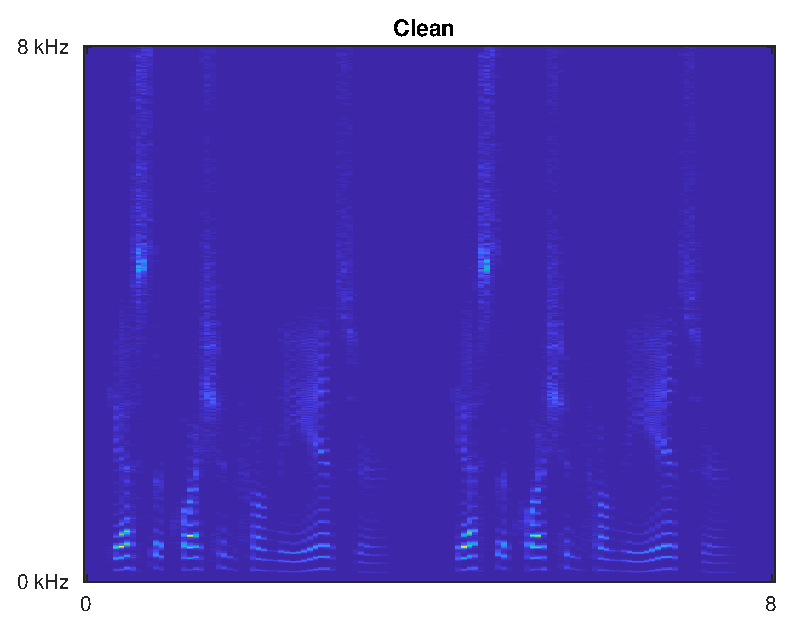
\includegraphics[width = 0.5\linewidth, height = 4cm]{fig/STFT/Sample_mjar0_clean.eps}} &
\subfloat[]{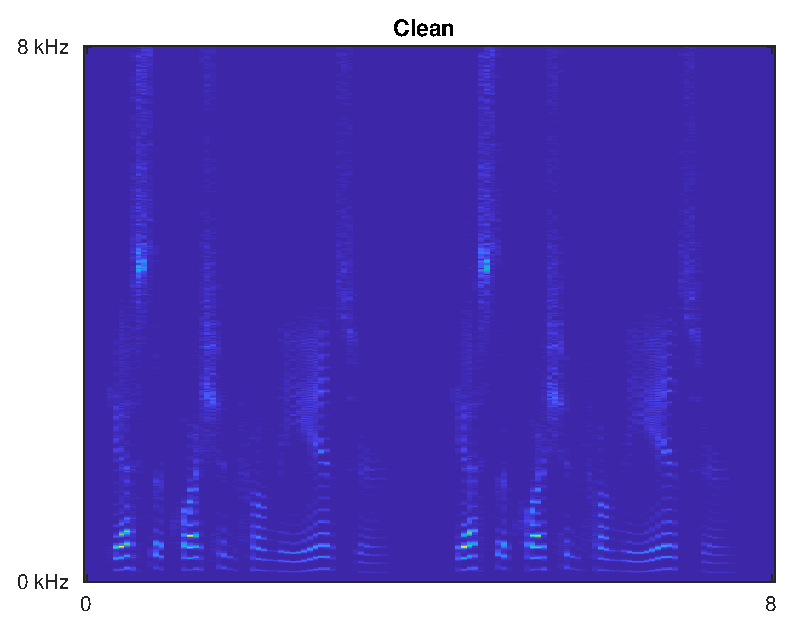
\includegraphics[width = 0.5\linewidth, height = 4cm]{fig/STFT/Sample_mjar0_clean.eps}}\\
\subfloat[]{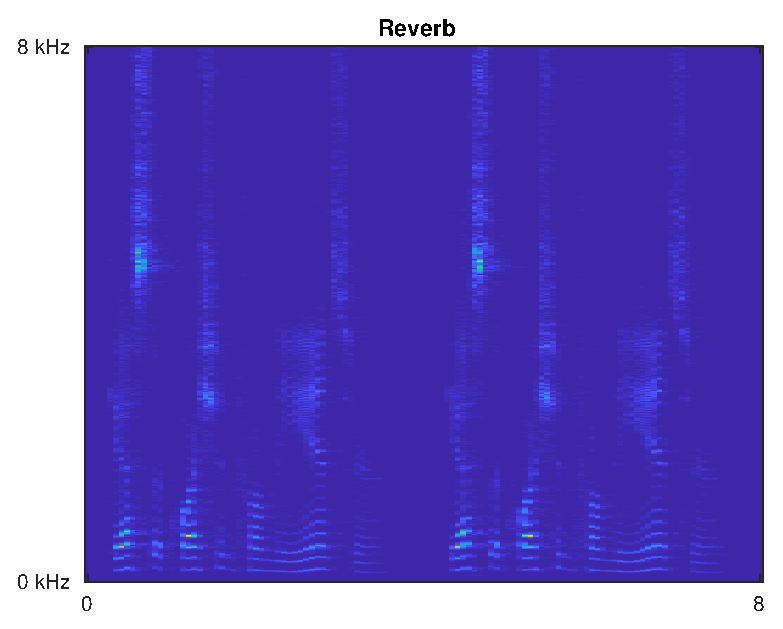
\includegraphics[width = 0.5\linewidth, height = 4cm]{fig/STFT/Sample_mjar0_reverb_RIR_SimRoom2_near_AnglA.eps}}&
\subfloat[]{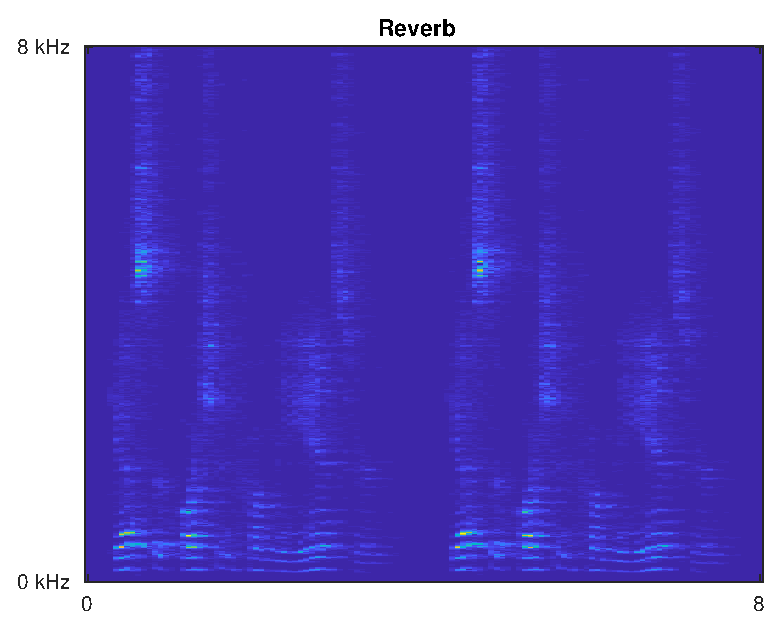
\includegraphics[width = 0.5\linewidth, height = 4cm]{fig/STFT/Sample_mjar0_reverb_RIR_SimRoom2_far_AnglA.eps}}\\
\subfloat[]{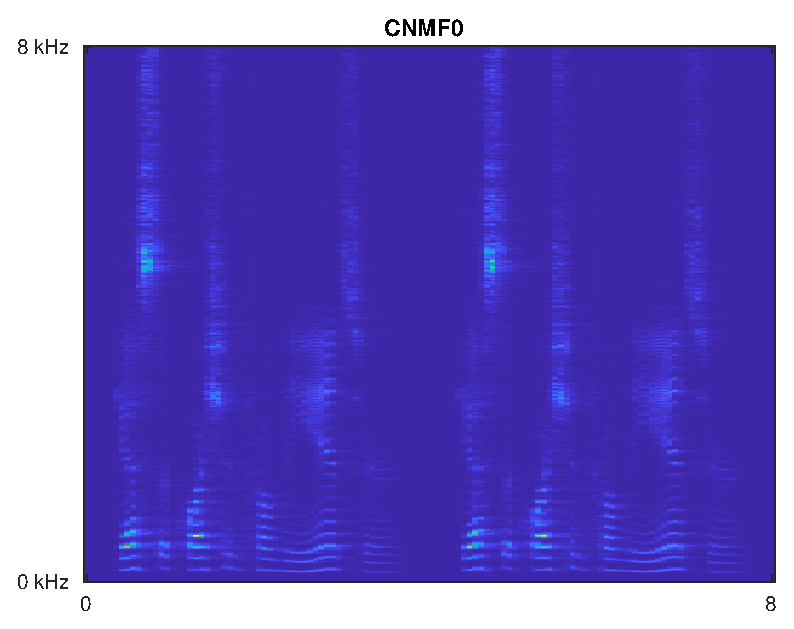
\includegraphics[width = 0.5\linewidth, height = 4cm]{fig/STFT/Sample_mjar0_CNMF0_RIR_SimRoom2_near_AnglA.eps}} &
\subfloat[]{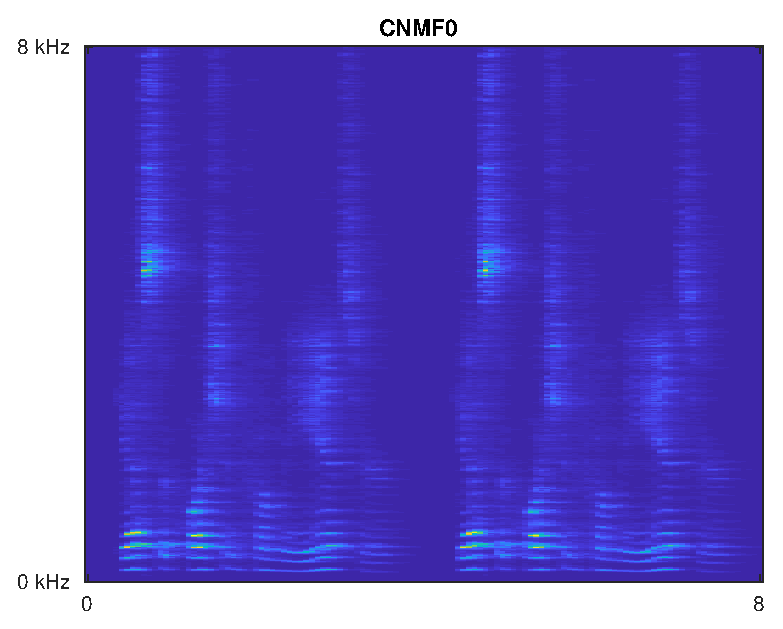
\includegraphics[width = 0.5\linewidth, height = 4cm]{fig/STFT/Sample_mjar0_CNMF0_RIR_SimRoom2_far_AnglA.eps}} \\
\subfloat[]{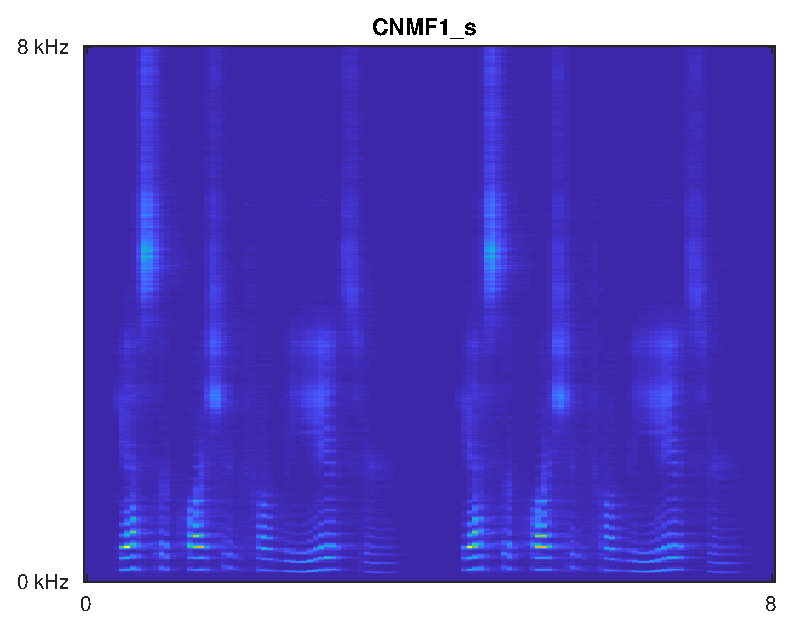
\includegraphics[width = 0.5\linewidth, height = 4cm]{fig/STFT/Sample_mjar0_SD_CNMF1_s_RIR_SimRoom2_near_AnglA.eps}}&
\subfloat[]{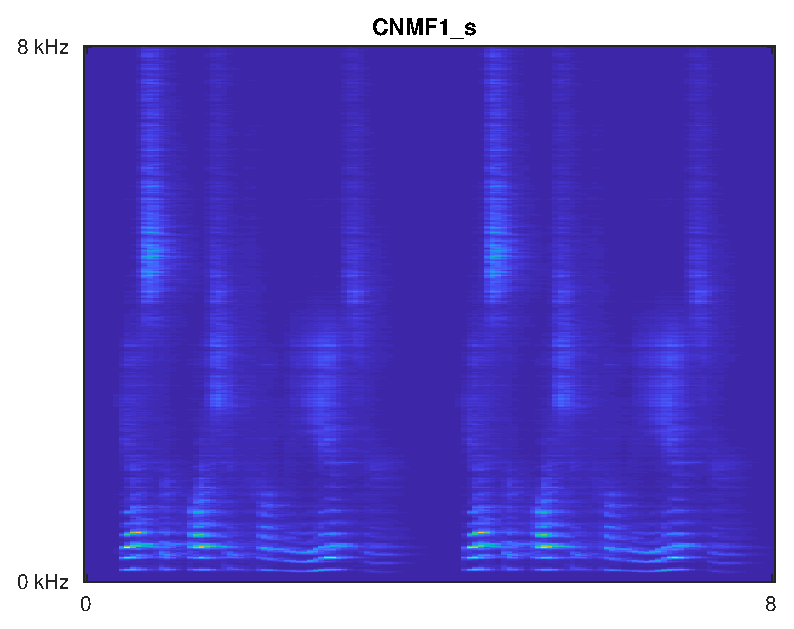
\includegraphics[width = 0.5\linewidth, height = 4cm]{fig/STFT/Sample_mjar0_SD_CNMF1_s_RIR_SimRoom2_far_AnglA.eps}}\\
\subfloat[]{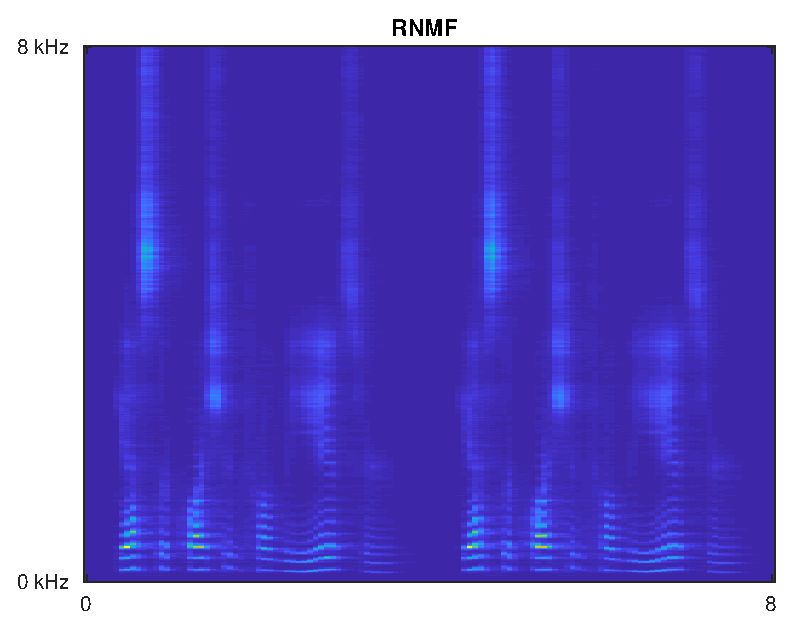
\includegraphics[width = 0.5\linewidth, height = 4cm]{fig/STFT/Sample_mjar0_SD_RNMF_RIR_SimRoom2_near_AnglA.eps}}&
\subfloat[]{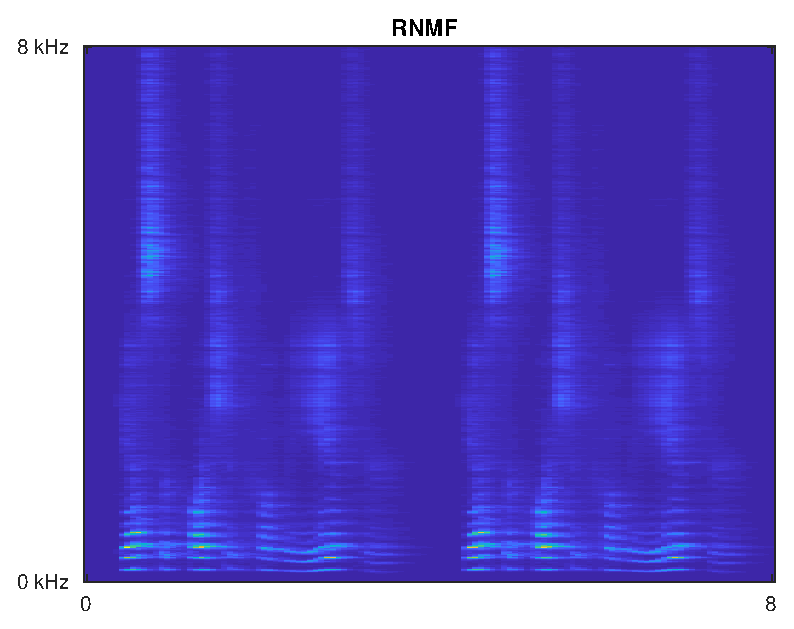
\includegraphics[width = 0.5\linewidth, height = 4cm]{fig/STFT/Sample_mjar0_SD_RNMF_RIR_SimRoom2_far_AnglA.eps}}\\
\end{tabular}
\caption[abc]{Comparison of reverb spectrogram estimated using various reverberation model when SD clean speech bases are used. Models are a smoother version of original spectrogram. The modeling error for all algorithms are small for near case. RNMF is more smoother than CNMF0. Spectrogram estimated using RNMF is mostly same as done by \text{CNMF1\_s}. }
\label{fig:Spectrogram_reverb_with_SD_bases}
\end{figure*}

\begin{figure*}
\begin{tabular}{cc}
\subfloat[]{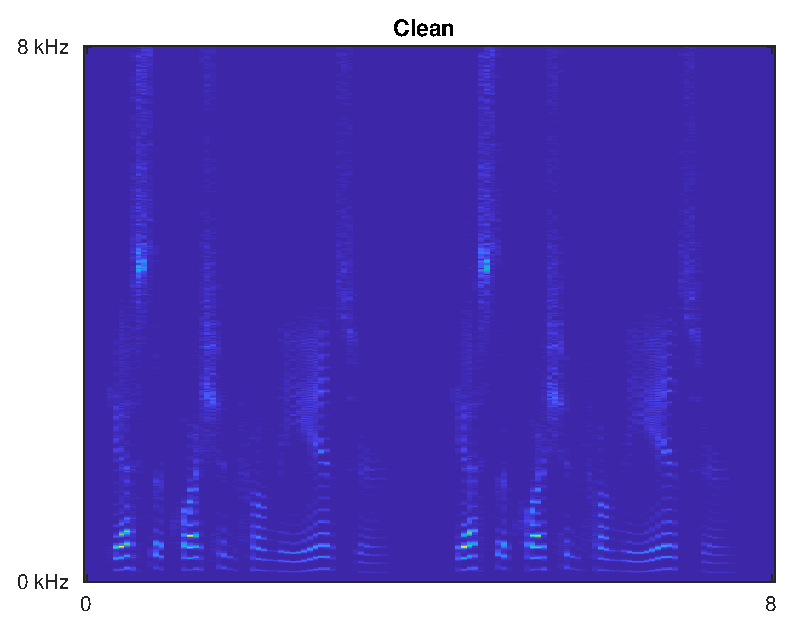
\includegraphics[width = 0.5\linewidth, height = 4cm]{fig/STFT/Sample_mjar0_clean.eps}} &
\subfloat[]{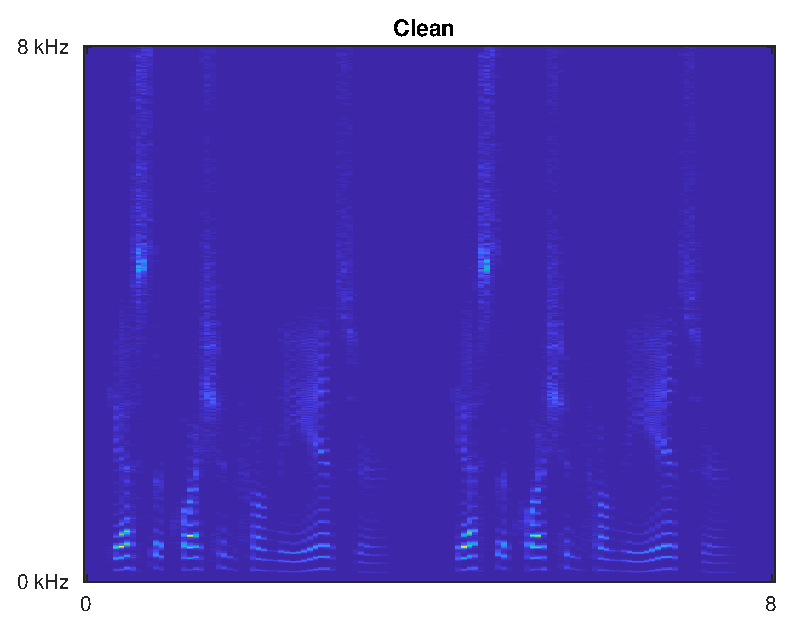
\includegraphics[width = 0.5\linewidth, height = 4cm]{fig/STFT/Sample_mjar0_clean.eps}}\\
\subfloat[]{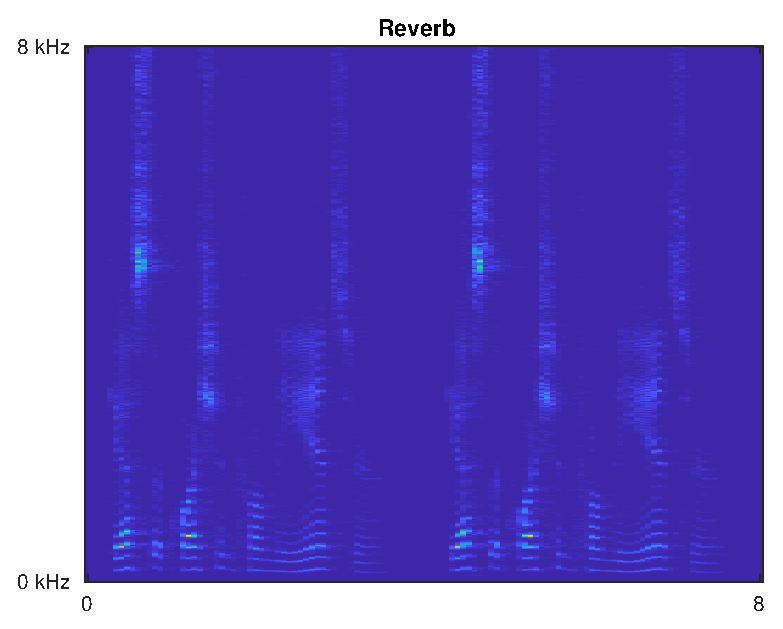
\includegraphics[width = 0.5\linewidth, height = 4cm]{fig/STFT/Sample_mjar0_reverb_RIR_SimRoom2_near_AnglA.eps}}&
\subfloat[]{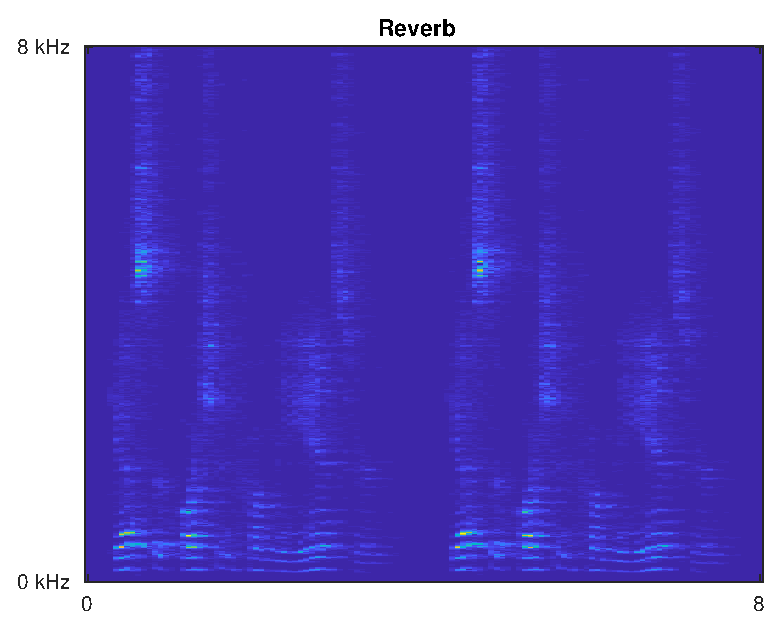
\includegraphics[width = 0.5\linewidth, height = 4cm]{fig/STFT/Sample_mjar0_reverb_RIR_SimRoom2_far_AnglA.eps}}\\
\subfloat[]{\includegraphics[width = 0.5\linewidth, height = 4cm]{fig/STFT/Sample_mjar0_CNMF0_RIR_SimRoom2_near_AnglA.eps}} &
\subfloat[]{\includegraphics[width = 0.5\linewidth, height = 4cm]{fig/STFT/Sample_mjar0_CNMF0_RIR_SimRoom2_far_AnglA.eps}} \\
\subfloat[]{\includegraphics[width = 0.5\linewidth, height = 4cm]{fig/STFT/Sample_mjar0_SI_CNMF1_s_RIR_SimRoom2_near_AnglA.eps}}&
\subfloat[]{\includegraphics[width = 0.5\linewidth, height = 4cm]{fig/STFT/Sample_mjar0_SI_CNMF1_s_RIR_SimRoom2_far_AnglA.eps}}\\
\subfloat[]{\includegraphics[width = 0.5\linewidth, height = 4cm]{fig/STFT/Sample_mjar0_SI_RNMF_RIR_SimRoom2_near_AnglA.eps}}&
\subfloat[]{\includegraphics[width = 0.5\linewidth, height = 4cm]{fig/STFT/Sample_mjar0_SI_RNMF_RIR_SimRoom2_far_AnglA.eps}}\\
\end{tabular}
\caption[abc]{Comparison of reverb spectrogram estimated using various reverberation model when SI clean speech bases are used. Models are a smoother version of original spectrogram. The modeling error for all algorithms are small for near case. RNMF is more smoother than CNMF0. Spectrogram estimated using RNMF is mostly same as done by \text{CNMF1\_s}. }
\label{fig:Spectrogram_reverb_with_SI_bases}
\end{figure*}
\fi
% use section* for acknowledgment
\section*{Acknowledgment}
Authors acknowledge the support by Council of Scientific and Industrial
Research (CSIR), India and Tata Consultancy Services (TCS), India

% Can use something like this to put references on a page
% by themselves when using endfloat and the captionsoff option.

%\ifCLASSOPTIONcaptionsoff
%  \newpage
%\fi

%\bibliographystyle{IEEEtran}
%\bibliography{NMF}

\iffalse
\begin{IEEEbiography}{Michael Shell}
Biography text here.
\end{IEEEbiography}

% if you will not have a photo at all:
\begin{IEEEbiographynophoto}{John Doe}
Biography text here.
\end{IEEEbiographynophoto}

% insert where needed to balance the two columns on the last page with
% biographies
%\newpage

#\begin{IEEEbiographynophoto}{Jane Doe}
#Biography text here.
#\end{IEEEbiographynophoto}
\fi

%\end{document}
\fi


%
\chapter{Materials and Methods}

\section{Including Figures}

Figures are conveniently included using postscript format.  If you are
generating a figure in a software, please check if the software
supports writing to a postscript or a PDF format. This format is loss
less vector format and with reproduce in any magnification without any
pixelation. Make sure to write it to an ``Encapsulated Post-script''or
.eps format.


\begin{figure}[tbp]
  \centering
    \includegraphics[width=0.7\textwidth]{profflow}
    \caption[Process flow sheet]{Process flow sheet of the
      experimental setup. The caption of the figure goes here. A
      shorter caption can be written in square brackets to identify it
      in the list of figures.}
    \label{fig:pfs} 
\end{figure}

Figures should be given a label and which can be used to refer to them
in the running text using \verb|\ref{}| command. Figure~\ref{fig:pfs}
describes the process flow sheet of the experimental set up used in
this report. The \Figref{fig:pfs} can also be refered by a short form notation
a pre-defined macro \verb"\Figref".



%%% Local Variables: 
%%% mode: latex
%%% TeX-master: "../mainrep"
%%% End: 

\chapter{Conclusion and suggestion for future work}
\label{chapter:conclusion}

\begin{itemize}
\item Conclusions

\item Future scope
\end{itemize}


%****************************************************************
%                         Appendices                           
%****************************************************************
%% Additional, supporting material, such as codes, derivations, etc., can be placed in the appendix
\appendix
\chapter{Supporting Material}

%******************************************************************
%                         Bibliography or References          
%******************************************************************  
\bibliography{NMF}     

%*******************************************************************
%                         List of publications               
%******************************************************************
%%%
\listofpublications


\noindent Put your publications from the thesis here. The packages \texttt{multibib} or \texttt{bibtopic} or \texttt{biblatex} or enumerate environment or thebibliography environment etc. can be used to handle multiple different bibliographies in the document.








%%======================================================================
%%% Local Variables: 
%%% mode: latex
%%% TeX-master: "../mainrep"
%%% End: 







            

%*******************************************************************
%                        Acknowledgements                    
%******************************************************************* 
%%%
\acknowledgments

This section is for the acknowledgments. Please keep this brief and resist the temptation of writing flowery prose! Do include all those who helped you, e.g. other faculty/staff you consulted, colleagues who assisted etc.






\signature{\today}
%\signature[Indian Institute of Technology Bombay]{\today}

%========================================================================

%%% Local Variables: 
%%% mode: latex
%%% TeX-master: "../mainrep"
%%% End:            

%*******************************************************************
%                        About author                    
%*******************************************************************
%\colophon % remove this command while using this file.

%*******************************************************************
\end{document}

%%% Local Variables: 
%%% mode: latex
%%% TeX-master: t
%%% End: 
